% --------------------------------------------------------------
% This is all preamble stuff that you don't have to worry about.
% Head down to where it says "Start here"
% --------------------------------------------------------------
\documentclass[12pt]{article}
\usepackage[spanish]{babel}
\usepackage[utf8x]{inputenc}
\usepackage{amsmath}
\usepackage{graphicx}
\usepackage[colorinlistoftodos]{todonotes}
\usepackage{color}
\usepackage{subfigure}
\usepackage{enumitem}
\usepackage{algpseudocode}
\providecommand{\abs}[1]{\lvert#1\rvert}
\providecommand{\norm}[1]{\lVert#1\rVert}
\sloppy
\definecolor{lightgray}{gray}{0.5}
\setlength{\parindent}{0pt}
\usepackage[margin=1in]{geometry} 
\usepackage{amsmath,amsthm,amssymb}
 
\newcommand{\N}{\mathbb{N}}
\newcommand{\Z}{\mathbb{Z}}
 
\newenvironment{theorem}[2][Theorem]{\begin{trivlist}
\item[\hskip \labelsep {\bfseries #1}\hskip \labelsep {\bfseries #2.}]}{\end{trivlist}}
\newenvironment{lemma}[2][Lemma]{\begin{trivlist}
\item[\hskip \labelsep {\bfseries #1}\hskip \labelsep {\bfseries #2.}]}{\end{trivlist}}
\newenvironment{exercise}[2][Exercise]{\begin{trivlist}
\item[\hskip \labelsep {\bfseries #1}\hskip \labelsep {\bfseries #2.}]}{\end{trivlist}}
\newenvironment{reflection}[2][Reflection]{\begin{trivlist}
\item[\hskip \labelsep {\bfseries #1}\hskip \labelsep {\bfseries #2.}]}{\end{trivlist}}
\newenvironment{proposition}[2][Proposition]{\begin{trivlist}
\item[\hskip \labelsep {\bfseries #1}\hskip \labelsep {\bfseries #2.}]}{\end{trivlist}}
\newenvironment{corollary}[2][Corollary]{\begin{trivlist}
\item[\hskip \labelsep {\bfseries #1}\hskip \labelsep {\bfseries #2.}]}{\end{trivlist}}
 
\begin{document}
 
% --------------------------------------------------------------
%                         Start here
% --------------------------------------------------------------
 
%\renewcommand{\qedsymbol}{\filledbox}

\title{Trabajo de estatica en \LaTeX}

\author{Beicker Baena Baldiris \and Yeison Sarmiento Lopez \and Yair Franco Puello \and 'Alvaro Polo Ulloque\and\ Dayana Jimenez Perez} 

\begin{titlepage}

\newcommand{\HRule}{\rule{\linewidth}{0.5mm}} % Defines a new command for the horizontal lines, change thickness here

\center % Center everything on the page
 
%----------------------------------------------------------------------------------------
%	HEADING SECTIONS
%----------------------------------------------------------------------------------------

\textsc{\LARGE Universidad Cat\'olica San pablo}\\[1.5cm] % Name of your university/college
\textsc{\Large Matem\'atica para la Computaci\'on}\\[0.5cm] % Major heading such as course name
\textsc{\large }\\[0.5cm] % Minor heading such as course title

%----------------------------------------------------------------------------------------
%	TITLE SECTION
%----------------------------------------------------------------------------------------

\HRule \\[0.4cm]
{ \huge \bfseries Lista de Ejercicios Nro.2 }\\[0.4cm] % Title of your document
\HRule \\[1.5cm]
 
%----------------------------------------------------------------------------------------
%	AUTHOR SECTION
%----------------------------------------------------------------------------------------

\begin{minipage}{0.4\textwidth}
\begin{flushleft} \large
\emph{Entregado por:}\\
Choqueluque Roman, David\\Flores Benites, Victor \\Moreno Vera, Felipe Adrian \\Palomino Paucar, Daniel \\Ramos Cooper, Solange \\% Your name
\end{flushleft}
\end{minipage}
~
\begin{minipage}{0.4\textwidth}
\begin{flushright} \large
\emph{Profesor:} \\
Sergio \textsc{Aquise Escobedo} % Supervisor's Name
\end{flushright}
\end{minipage}\\[2cm]

% If you don't want a supervisor, uncomment the two lines below and remove the section above
%\Large \emph{Author:}\\
%John \textsc{Smith}\\[3cm] % Your name

%----------------------------------------------------------------------------------------
%	DATE SECTION
%----------------------------------------------------------------------------------------

{\large \today}\\[2cm] % Date, change the \today to a set date if you want to be precise

\vfill % Fill the rest of the page with whitespace

\end{titlepage}

\newpage

%=========================================================
% BISWA DATA
%=========================================================
% 
% Sección 5
% °°°°°°°°°°°°°°°°°°°°°°°°°°°°°°°°°°°°°°°°°°°°°°°°°°°°°°°°
\section{Biswa Datta: secciones 5.2 y 5.3}

% Ejercicio 1
\subsection{Ejercicio 1}
\begin{enumerate}
    \item Mostrar que una matriz triangular inferior elemental tiene la forma:\\
    
        $$E = I + m_{k}e_{k}^{T}$$
        donde $m_{k}=(0,0,...,0,m_{k+1,k}, ..., m_{n,k})^{T} $
        
        Solución:
        
        \(
            A =
            \left( {\begin{array}{c}
                a_{1} \\
                a_{2} \\
                ... \\
                a_{n}\\
            \end{array} } \right)
        \)
        
        $$a_{1} \neq 0 $$
        
        tomamos también que $e_{i}^{T}m_{k} = 0$ para $i = 1, 2, ..., k$
        Esto podemos ver de la siguiente matriz:
        
        \[
        E =
            \left( {\begin{array}{cccccccc}
                1 & 0  & 0 & 0 & ... & 0 & 0 & 0\\
                0 & 1  & 0 & 0 & ... & 0 & 0 & 0\\
                0 & 0  & 1 & 0 & ... & 0 & 0 & 0\\
                ... & ... & ... & ... & ... & ... & ... & ...\\
                ... & ... &  & 0 & 1 & ... &  & ...\\
                0 & 0  & 0 & ... & m_{k+1,k} & ... & 0 & 0\\
                0 & 0  & 0 & ... & ... & ... & ... & 0\\
                0 & 0  & 0 & ... & m_{n,k} & ... & 0 & 1\\
            \end{array} } \right)
        \]
        
        
        Decimos que existe una matriz elementaria E tal que  $E_{a}$ es múltiplo de $e_{1}$
        \[
        E =
            \left( {\begin{array}{cccccc}
                1 & 0  & 0 & ... & ... & 0\\
                -\frac{a_{2}}{a_{1}} & 1  & 0 & ... & ... & 0\\
                ... & 0 & ... & ... & ... & 0 \\
                ... & ... & ... & ... & ... & ... \\
                ... & ... & ... & ... & ... & ... \\
                -\frac{a_{n}}{a_{1}} & 0 & 0 & ... & 0 & 1 \\
            \end{array} } \right)
        \]
        
        tiene la forma de una matriz triangular inferior tal que:
        
        \(
            E_{a} =
            \left( {\begin{array}{c}
                a_{1} \\
                0 \\
                0 \\
                ... \\
                ... \\
                0\\
            \end{array} } \right)
        \)
        
        De esta forma si juntamos todos los $m_{k}E_{k}^{T}, para k = 1 ... n$, obtenemos
    
        \[
        E =
            \left( {\begin{array}{cccccccc}
                1 & 0  & 0 & 0 & ... & 0 & 0 & 0\\
                m_{1,0} & 1  & 0 & 0 & ... & 0 & 0 & 0\\
                m_{2,0} & m_{2,1}  & 1 & 0 & ... & 0 & 0 & 0\\
                ... & ... & ... & 1 & ... & ... & ... & ...\\
                ... & ... & ... & ... & 1 & ... &  & ...\\
                ... & ...  & ... & ... & m_{k+1,k} & ... & 0 & 0\\
                ... & ...  & ... & ... & ... & ... & ... & 0\\
                m_{n,0} & m_{n,1}  & m_{n,2} & ... & m_{n,k} & ... & m_{n,n-1} & 1\\
            \end{array} } \right)
        \]
        
        Tiene la forma matriz triangular inferior.
        
    \item Mostrar que la inversa de  E en (a) es dada por:\\
    
        $$E^{-1} = I - m_{k}e_{k}^{T}$$
    
        Si suponemos que $$E^{-1} = I - m_{k}e_{k}^{T}$$ y $$E = I + m_{k}e_{k}^{T}$$, por tanto $$E * E^{-1} = I$$
        \begin{align*}
            E * E^{-1} &= I \\
            (I + m_{k}e_{k}^{T})*(I - m_{k}e_{k}^{T}) &= I\\
            I*I + I*(m_{k}e_{k}^{T}) - i*(m_{k}e_{k}^{T}) - (m_{k}e_{k}^{T}) *(m_{k}e_{k}^{T}) &= I\\
            I - (m_{k}e_{k}^{T}) *(m_{k}e_{k}^{T}) &= I\\
            - (m_{k}e_{k}^{T}) *(m_{k}e_{k}^{T}) &= I - I\\
            - (m_{k}e_{k}^{T}) *(m_{k}e_{k}^{T}) &= 0\\
        \end{align*}
\end{enumerate}





 % Walter

% Ejercicio 4
\subsection{Ejercicio 4}
Sean $A$ una matriz simétrica definida positiva. Al finalizar el primer paso de la factorización $LU$ de $A$ tenemos:

$$
A^{(1)} = \begin{pmatrix}
            a_{11} & a_{12} & ... & a_{1n} \\ 
            0 & & & \\
            0 & & & \\
            . & & & \\
            . & & A^{'} & \\
            . & & & \\
            0 & & & \\
        \end{pmatrix}
$$

Pruebe que $A^{'}$ es simétrica y definida positiva. Entonces muestre que la factorización $LU$ de una matriz simétrica definida positiva usando eliminación Gaussiana sin pivoteo siempre existe y es única.\\

\noindent \textcolor{red}{\bf Solución:\\}

Sea:

$$
A = \begin{pmatrix}
    a_{11} & a_{12} & ... & a_{1n} \\
    a_{21} & a_{22} & ... & a_{2n} \\
    ... & ... & ... & ... \\
    a_{n1} & a_{n2} & ... & a_{nn} \\
\end{pmatrix}
$$

una matriz simétrica y definida positiva y 

$$
m_1 = \begin{pmatrix}
    0 \\
    a_{21} \\
    ... \\
    a_{n1}
\end{pmatrix}
$$

siendo $M_1=I-m_1e_1^{t}$

$$
M_1 = \begin{pmatrix}
    1 & 0 & ... & 0 \\
    \frac{-a_{21}}{a_{11}} & 1 & ... & 0 \\
    ... & ... & ... & ... \\
    \frac{-a_{n1}}{a_{11}} & 0 & ... & 1 \\
\end{pmatrix}
$$

Entonces:

$$
A_1 = M_1*A
$$

$$
A_1 = \begin{pmatrix}
    1 & 0 & ... & 0 \\
    \frac{-a_{21}}{a_{11}} & 1 & ... & 0 \\
    ... & ... & ... & ... \\
    \frac{-a_{n1}}{a_{11}} & 0 & ... & 1 \\
\end{pmatrix} * \begin{pmatrix}
    a_{11} & a_{12} & ... & a_{1n} \\
    a_{21} & a_{22} & ... & a_{2n} \\
    ... & ... & ... & ... \\
    a_{n1} & a_{n2} & ... & a_{nn} \\
\end{pmatrix}
$$

$$
A_1 = \begin{pmatrix}
            a_{11} & a_{12} & ... & a_{1n} \\ 
            0 & & & \\
            0 & & & \\
            . & & & \\
            . & & A^{'} & \\
            . & & & \\
            0 & & & \\
        \end{pmatrix}
$$

Operando:

$$
A^{'} = \begin{pmatrix}
    \frac{-a_{21}a_{12}}{a_{11}}+a_{22} & \frac{-a_{21}a_{13}}{a_{11}}+a_{23} & ... & \frac{-a_{21}a_{1n}}{a_{11}}+a_{2n} \\
    \frac{-a_{31}a_{12}}{a_{11}}+a_{32} & \frac{-a_{31}a_{13}}{a_{11}}+a_{33} & ... & ...\\
    ... & ... & ... & ... \\
    \frac{-a_{n1}a_{12}}{a_{11}}+a_{n2} & ... & ... & ... \\
\end{pmatrix}
$$

Pero dado que $A$ era simétrica y definida positiva, entonces $a_{ij}=a_{ji}$, por lo tanto del cálculo anterior se demuestra que $A^{'}$  también es simétrica y definida positiva.

 % Daniel

% Ejercicio 6
\subsection{Ejercicio 6}
Asumiendo que la factorización LU de $A$ existe, probar que:
\begin{enumerate}
    \item $A$ puede ser escrito en la forma\\
    $$
     A = LDU_1
    $$
    donde $D$ es una matriz diagonal y $L$, $U_1$ son matrices triangular inferior y superior respectivamente.\\\\
    \textbf{Solución}\\
    Creamos una matriz $D$ diagonal formado por los elementos de la diagonal de la matriz $U$, tal que $d_{ii} = u_{ii} \forall i \in 1, \ldots, n$. Así $A = LU = L(DD^{-1})U = LD(D^{-1}U)$, donde $D^{-1}$ es una matriz diagonal tal que $d_{ii}^{-1} = \frac{1}{d_ii^{i-1}}$ además se sabe que el producto de una matriz diagonal por una triangular superior sigue siendo una matriz triangular superior. Luego tenemos una nueva matriz $U_1$ denotado por:
    $$
    U_1 = D^{-1}U
    $$
    
    Reemplazando $U$ con $U_1$:
    
    $$
    A = LDU_1
    $$
    
    Visualmente:
    
    \[
        D = \begin{bmatrix}
            d_{11} & 0 & \ldots & 0 \\
            0 & d_{22} & \ldots & 0 \\
            \vdots & \vdots & \ddots & \vdots\\
            0 & 0 & \ldots & d_{nn}\\
        \end{bmatrix}
        ,
        D^{-1} = \begin{bmatrix}
            \frac{1}{d_{11}} & 0 & \ldots & 0 \\
            0 & \frac{1}{d_{22}} & \ldots & 0 \\
            \vdots & \vdots & \ddots & \vdots\\
            0 & 0 & \ldots & \frac{1}{d_{nn}}\\
        \end{bmatrix}
    \]
    
    \[
        U_1 = \begin{bmatrix}
            1 & \frac{d_{12}}{d_{11}} & \frac{d_{13}}{d_{11}} & \ldots & \frac{d_{1n}}{d_{11}}\\
            0 & 1 & \frac{d_{23}}{d_{22}} & \ldots & \frac{d_{2n}}{d_{22}}\\
            0 & 0 & 1 & \ldots & \vdots\\
            \vdots & \vdots & \vdots & \ddots & \vdots\\
            0 & 0 & 0 & 0& 1\\
        \end{bmatrix}
    \]
    
    \item Si $A$ es simétrico luego:
    $$
    A = LDL^T
    $$\\\\
    
    \textbf{Solución}\\
    Usando la factorización de $a)$ tenemos que $A = LDU_1$ si le aplicamos la transpuesta a ambos lados y tenemos:
    
    \begin{center}
            $A^T = (LDU_1)^T$\\
            $A^T = U_1^T DL^T$\\
   \end{center}

\textrm{Como A es simétrica además que $-m_{21} = \frac{a_{21}}{a_{11}} = \frac{a_{12}}{a_{11}}= -m_{12}$ luego tenemos que:}\\
    
    \begin{equation*}
        \begin{split}
            A &= LDL^T
        \end{split}
    \end{equation*}
    
    \item Si $A$ es simétrico y definido positivo, luego
    $$
    A = HH^T
    $$
    
    donde $H$ es una matriz triangular inferior con entradas diagonales positivas (conocido como la \textit{descomposición de Cholevsky})\\\\
    \textbf{Solución}\\
    
    \textbf{Definición}
    Si $x$ es un autovector de $A$ luego $x \neq 0$ y $A x = \lambda X$. En este caso $x^TAx = \lambda x^T x$. Si $\lambda > 0$ tenemos que $x^T A x > 0$. Luego sabemos que una matriz es positiva definida si $x^TAx > 0$ para todos los vectores $x \neq 0$.
    
    Del problema (b) tenemos la matriz $A = LDL^T$, la cual la podemos reescribir como $D = L^{-1}AL^{-1}$. La matriz $D$ por la definición anterior será una nueva matriz definida positiva. Así los elementos de la matriz diagonal de la matriz $D$ serán positivos y de la forma $d_{ii} > 0 \forall i = 1, \ldots, n$.
    
    Luego creamos una matriz $D'$, tal que $D' = diag(\sqrt{d_1}, \ldots \sqrt{d_n})$ y denotamos $H = LD'$. Así:
    \begin{equation*}
        \begin{split}
            H H^T &= (L D')(L D')^T\\
            &= (L D')(D')^T L^T\\
            &= L(D'D'^T)L^T\\
            &= L D L ^T
        \end{split}
    \end{equation*}
\end{enumerate} % Josué

% Ejercicio 7
\subsection{Ejercicio 7}
Suponiendo que exista la factorización $LU$ de $A$, desarrolle un algoritmo para calcular $U$ por filas y $L$ por columnas directamente de la ecuación:
\[
    A = LU
\]
Esto se conoce como reducción de Doolittle.

\textbf{Solución:}

Para cada $k=1,2,...,n$:
\[
    u_{k, m} = a_{k, m} - \sum_{j=1}^{k-1} l_{k,j} u_{j,m}
\]
\[
    l_{i, k} = \frac{(a_{i, k} - \sum_{j=1}^{k-1} l_{i,j} u_{j, k})}{u_{kk}}
\]
El siguiente ejemplo nos permitirá verificar el algoritmo basado en el metodo de Doolittle; sea:

\[
    A = \begin{bmatrix}a_{1,1} & a_{1,2} & a_{1,3}\\ a_{2,1} & a_{2,2} & a_{2,3}\\ a_{3,1} & a_{3,2} & a_{3,3} \end{bmatrix}
\]
Para $k=1$, tenemos:

\[
    u_{1, 1} = a_{1, 1} - \sum_{j=1}^{0} l_{1,j} u_{j, 1} = a_{1, 1} \quad ( m = 1 )
\]
\[
    u_{1, 2} = a_{1, 2} - \sum_{j=1}^{0} l_{1,j}u_{j, 2} = a_{1,2} \quad ( m = 2 )
\]
\[
    u_{1, 3} = a_{1, 3} - \sum_{j=1}^{0} l_{1, j} u_{j, 3} = a_{1, 3} \quad ( m = 3 )
\]
\[
    l_{1, 1} = 1
\]
\[
    l_{2, 1} = \frac{a_{2, 1} - \sum_{j=1}^{0} l_{2,j}u_{j,1}}{u_{1,1}} = \frac{a_{2, 1}}{u_{1, 1}} \quad (i = 2)
\]
\[
    l_{3, 1} = \frac{a_{3, 1} - \sum_{j=1}^{0} l_{3,j}u_{j,1}}{u_{1, 1}} = \frac{a_{3, 1}}{u_{1, 1}} \quad (i = 3)
\]

Para $k=2$, tenemos:
\[
    u_{2, 2} = a_{2, 2} - \sum_{j=1}^{1} l_{2,j} u_{j,2} = a_{2, 2} - l_{2, 1}u_{1, 2} \quad (m = 2)
\]
\[
    u_{2, 3} = a_{2, 3} - \sum_{j=1}^{1} l_{2, j} u_{j, 3} = a_{2, 3} - l_{2, 1} u_{1, 3} \quad (m = 3)
\]
\[
    l_{2, 2} = 1
\]
\[
    l_{3, 2} = \frac{a_{3, 2} - \sum_{j=1}^{1} l_{3,j} u_{j, 2}}{u_{2, 2}} = \frac{a_{3, 2} - l_{3, 1} u_{1, 2}}{u_{2, 2}}
\]

Para $k=3$, tenemos:
\[
    u_{3, 3} = a_{3, 3} - \sum_{j=1}^{2} l_{3, j} u_{j, 3} = a_{3, 3} - l_{3, 1} u_{1, 3} - l_{3, 2} u_{2, 3} \quad (m = 3)
\]
\[
    l_{3, 3} = 1
\]
El algoritmo termina en este punto.\\
Obtenemos las siguientes ecuaciones para las entradas en U:
\[
    u_{1, 1} = a_{1, 1}
\]
\[
    u_{1, 2} = a_{1, 2}
\]
\[
    u_{1, 3} = a_{1, 3}
\]
\[
    u_{2, 2} = a_{2, 2} - l_{2, 1} u_{1, 2}
\]
\[
    u_{2, 3} = a_{2, 3} - l_{2, 1} u_{1, 3}
\]
\[
    u_{3, 3} = a_{3, 3} - l_{3, 1} u_{1, 3} - l_{3, 2} u_{2, 3}
\]
Y obtenemos las siguientes ecuaciones para las entradas en U:
\[
    l_{2, 1} = \frac{a_{2, 1}}{u_{1, 1}}
\]
\[
    l_{3, 1} = \frac{a_{3, 1}}{u_{1, 1}}
\]
\[
    l_{3, 2} = \frac{a_{3, 2} - l_{3, 1} u_{1, 2}}{u_{2, 2}}
\]
Además, $l _{1, 1} = l_{2, 2} = l_{3, 3} = 1$
     % Roxana

% Ejercicio 8
\subsection{Ejercicio 8}
Desarrollar un algoritmo que calcule la factorización
\[A=LU\]
donde U es la unidad triangular superior y L es triangular inferior. Se conoce como Cout reduction. Consejo:Derive el algorimo de la ecuación A= LU

\textbf{Solución:}

Teniendo en cuenta que A se puede factorizar como el producto de una matriz triangular inferior $L$ con una matriz triangular superior $U$.
\[A=LU\]
En este caso, el sistema de ecuaciones da: $Ax = B$
Entonces remplazandolo tenemos:
\[LUx=b\]
Si denominamos z a la matriz columna de n filas reultado del producto $Ux$, tenemos que la ecuación  $LUx=b$ se puede escribir del siguiente modo:
\[Lz = b\]
A partir de las ecuaciones $LUx = b$ y $Lz=b$ es posible plantear un algoritmo para resolver el sistema de ecuaciones empleando dos etapas:
- Primero obtenemos $z$ aplicando el algoritmo de sustitución progresiva en la ecuación $Lz=b$\\
- Posteriormente obtenemos los valores de $x$ aplicando el algoritmo de sustitución regresiva a la ecuación $Ux = z$\\
El análisis anterior nos muestra lo fácil que es resolver estos dos sistemas de ecuaciones triangulares y lo útil que resultaría disponer de un método que nos permita llevar a cabo la factorización $A= LU$. si disponemos de una matriz $a$ de $m x n$, estamos interesados en encontrar aquellas matrices:\\

\[ L =
\left(
\begin{array}{lcrcr}
l_{11} & 0 & 0 & ... & 0 \\
l_{21} & l_{22} & 0 & ... & 0 \\
l_{31} & l_{32} & l_{33} & ... &0 \\
: & : & : &  : & :\\
l_{n1} & l_{n2} & l_{n3} & ... &l_{nn} \\
\end{array}
\right)
\]
\[ U =
\left(
\begin{array}{lcrcr}
u_{11} & u_{12} & u_{13} & ... & u_{14} \\
0 & u_{22} & u_{23} & ... & u_{2n} \\
0 & 0 & u_{33} & ... &u_{3n} \\
: & : & : &  : & :\\
0 & 0 & 0 & ... &u_{nn} \\
\end{array}
\right)
\]
Tales que cumplan la ecuación $A=LU$. cuando esto es posible decimos que $A$ tien una descomposición $LU$. Se puede ver que la ecuación anterior no determina de forma única a $L$ y a $U$. Para cada $i$ podemos asignar un valor distinto de cero a $l_{ii}$ o $u_{ii}$ (aunque no ambos). Por ejemplo, una elección simple es fijar $l_{ii} = 1$ para $i=1,2,...,n$ haciendo de esto modo que $L$ sea una matriz triangular inferior unitaria. Otra elección es hacer $U$ una matriz triangular superior unitaria (tomando $U_{ii} = 1$ para cada $i$).\\
Para deducir un algoritmo que nos permita la factorización $LU$ de $A$ partiremos de la fórmula para la multiplicación de matrices:\\
\[a_{ij} = \sum_{s=1}^{n} l_{is}u_{sj} = \sum_{s=1}^{min(i,j)} l_{is}u_{sj}\]
En donde nos hemos valido del hecho de que $l_{is} = 0$ para $s>i$ y $u_{sj}=0$ para $s>j$.
En este proceso, cada paso determina una nueva fila de $U$ y una nueva columna de $L$. En el paso $k$, podemos suponer que ya se calcularon las filas $1,2,...,k-1$ de $U$, al igual que las columnas $1,2,...,k-1$ de $L$. Haciendo $i=j=k$ en la ecuación aterior obtenemos:
\[a_{kk} = l_{kk}u_{kk} \sum_{s=1}^{k-1}l_{ks}  u_{sk}\]
Si especificamos una valor para $l_{kk}$ (o para $u_{kk}$), a partir de la ecuación anterior es posible determinar un valor para el otro término. Conocidas $u_{kk}$ y $l_{kk}$ y apartir de la ecuación $a_{ij} = \sum_{s=1}^{n} l_{is}u_{sj} = \sum_{s=1}^{min(i,j)} l_{is}u_{sj}$ podemos escribir las expresiones para la k-ésima fila $(i=k)$ y para la k-ésima columna $(j=k)$, respectivamente:
\[a_{kj} = l_{kk} u_{kj} + \sum_{s=1}^{k-1} l_{ks} u_{sj}  (k+1 \leq j \leq n)\]  
\[a_{ik} = l_{ik} u_{kk} + \sum_{s=1}^{k-1} l_{is} u_{sk}  (k+1 \leq i \leq n)\]  
Esta última ecuación se puede emplear para encontrar los elementos $U_{kj}$ y $l_{ik}$
el algoritmo basado en el análisis anterior se denomina factorización de Doolittle cuando se toman los términos $l_{ii}=1$ para $1\leq i \leq n$ (L triangular inferior unitaria ) y factorización de Crout cuando se toman los términos $u_{ii} = 1$ (U triangular superior unitaria).\\
A continuación la implementación del algoritmo:\\\\
input $n,(a_{ij})$
\begin{algorithmic}	
	%input $n,(a_{ij})$
    \State{$n,(a_{ij})$}
	\For {k=1,2,...,n} 
		\State{Especificar un valor para $l_{kk}$ o $u_{kk}$ }
		\State{Calcular el otro término mediante:}
		\State{$l_{kk}u_{kk} = a_{kk} - \sum_{s=1}^{k-1} l_{ks} u_{sk}$}
		\For {$j=k+1, k+2, ... , n$}
			\State{$u_{kj} \longleftarrow ((a_{kj} - \sum_{s=1}^{k-1} l_{ks} u_{sk}) / l_{kk}$}
		\EndFor
	\EndFor
	\State output{ $(l_{ij}),(u_{ij})$}
\end{algorithmic} % Roxana

% Ejercicio 9
\subsection{Ejercicio 9}
Compare las reducciones de Dolittle y Crout con la eliminacion Gausiana con respecto a flop count, requerimientos de almacenamiento y posibilidad de acumulación de productos internos in double precision

\textbf{Solución}

Si definimos cada punto en cuestión:
\begin{itemize}
    \item Flops: Numero de operaciones de multiplicación y división que representan el esfuerzo numérico.
    \item Requerimientos de almacenamiento: Cantidad de almacenamiento necesario para realizar cálculos durante la ejecución del método.
    \item Acumulación de productos internos en precisión doble: Técnica para minimizar la propagación del error.
\end{itemize}

Eliminación Gaussiana.
El numero de flops del algoritmo es:
\begin{itemize}
    \item Bucle interno: "Convertir en cero los elementos abajo del pivote"
    $$\sum_{j=k+1}^{n}1=n-(k+1)\approx n-k$$
    \item Bucle intermedio: 'Calcular los multiplicadores de cada fila'
    $$\sum_{j=k+1}^{n}2+( \text{flops del bucle interno})=\sum_{j=k+1}^{n}2+(n-k)= (2+n-k)(n-k)$$
    $$=(n^2+2n)-2(n+1)k+k^2$$
    \item Bucle exterior: 
    $$\sum_{k=1}^{n-1}n^2+2n.2(n+1)k+k^2$$
    $$=(n^2+2n)\sum_{k=1}^{n-1}1-2(n+1)\sum_{k=1}^{n-1}k+\sum_{k=1}^{n-1}k^2$$
    $$=\frac{n^3}{3} + O(n^3)$$
\end{itemize}
En cuanto a los requerimientos de almacenamiento, el método sobrescribe en la misma matriz $nxn$ los valores obtenidos. Por lo que el método solo necesita almacenar una matriz de tamaño $nxn$ durante su ejecución.

Reduccion Dolittle:
Este método es una forma alternativa para descomponer una matriz en las matrices LU sin tener que utilizar eliminación Gaussiana.
\\ Sea la matriz $A_{nxn}$:
$$A=\begin{bmatrix}
    a_{1,1}&a_{1,2}&...&a_{1,n}\\
    a_{2,1}&a_{2,2}&...&a_{2,n}\\
    ...\\
    a_{n,1}&a_{n,2}&...&a_{n,n}
\end{bmatrix}$$
Asumimos que existen dos matrices $L$ y $U$ tal que:
$$A=LU$$
y las matrices $L$ y $U$ son de la forma:
$$U=\begin{bmatrix}
    u_{1,1}&l_{1,2}&...&u_{1,n}\\
    0&u_{2,2}&...&u_{2,n}\\
    ...\\
    0&0&...&u_{n,n}
\end{bmatrix}$$
$$L=\begin{bmatrix}
    1&0&...&0\\
    l_{2,1}&1&...&0\\
    ...\\
    l_{1,1}&l_{n,2}&...&1
\end{bmatrix}$$
El método de Dolittle calcula los valores $u_{i,j}$ y $l_{i,j}$ con el siguiente algoritmo: \\\\

% Mejor si lo pones en lenguaje Latex...
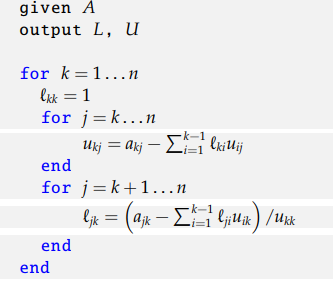
\includegraphics{images/dolittleAlg.PNG}

Si analizamos el algoritmo anterior:
\begin{itemize}
    \item Para el primer bucle (linea 3):
    $$\sum_{j=k}^{n}\sum_{i=1}^{k-1}1=\sum_{j=k}^{n}(k-1)=(k-1)(n-k)$$
    \item Para el segundo bucle interno (linea 9):
    $$\sum_{j=k+1}^{n}\sum_{i=1}^{k-1}1=\sum_{j=k+1}^{n}(k-1)$$
    $$=(n-k-1)(k-1)$$
    \item Para el bucle externo:
     $$\sum_{k=1}^{n}=(k-1)(n-k)+(n-k-1)(k-1)=\sum_{k=1}^{n}1 + k - 2 k^2 - 2 n + 2 k n$$
     Entonces el numero total de FLOPS seria:
     $$=(7 n)/6 - (3 n^2)/2 + n^3/3$$
     
     
\end{itemize}
En cuanto a los requerimientos de almacenamiento de este método, es necesario que durante todo el proceso de calculo se mantengan 3 matrices de tamaño $nxn$ que corresponden a las matrices: $A, L$ y $U$.

Método de Crout:

Este metodo es muy similar al método de Dolittle con la diferencia de que Crout retorna la descomposición LU de la matriz de la forma:
$$U=\begin{bmatrix}
    u_{1,1}&l_{1,2}&...&u_{1,n}\\
    0&u_{2,2}&...&u_{2,n}\\
    ...\\
    0&0&...&u_{n,n}
\end{bmatrix}$$
$$L=\begin{bmatrix}
    1&0&...&0\\
    l_{2,1}&1&...&0\\
    ...\\
    l_{1,1}&l_{n,2}&...&1
\end{bmatrix}$$
mientras que Crout retorna:
$$U=\begin{bmatrix}
    1&l_{1,2}&...&u_{1,n}\\
    0&1&...&u_{2,n}\\
    ...\\
    0&0&...&1
\end{bmatrix}$$
$$L=\begin{bmatrix}
    l_{1,1}&0&...&0\\
    l_{2,1}&l_{2,2}&...&0\\
    ...\\
    l_{1,1}&l_{n,2}&...&l_{n,n}
\end{bmatrix}$$
El conteo de flops del algoritmo de Crout es muy similar al metodo de Dolittle. Es decir $O(n^3/3)$.
En cuanto a los requerimientos de almacenamiento. Es necesario mantener 3 matrices $n$x$n$ que corresponden a las matrices $A,L$ y $U$.

Por lo tanto al comparar los 3 métodos tendríamos que:

\begin{itemize}
    \item Flops: Los 3 metodos realizan una cantidad total de FLOPS parecidas de orden $O(n^3/3)$.
    \item Requerimientos de almacenamiento: La eliminacion de Gauss utiliza la matriz original $n$x$n$. Tanto Dolittle como Crout utilizan 2 matrices $n$x$n$ que corresponden a las matrices $L$ y U, ademas de la matriz original.
    \item Acumulacion de productos internos en precision doble: Crout permite la acumulacion de productos internos en doble precision. Gauss no permite esto 
    
\end{itemize} % David

%Ejercicio 13
\subsection{Ejercicio 13}
%wilderd
\renewcommand{\labelenumi}{\alph{enumi}}
%%%% Sol
\begin{enumerate}[label=(\alph*)]
    \item Sea A de orden $mxn$ y sea $r = min\{ m-1,n\}$, desarrolle un algoritmo para construir las matrices elementales $E_1,\dots ,E_r$, tal que:
    \[
	E_r, E_{r-1}, \dots E_2, E_1 A
    \]
    es una matriz trapezoidal superior U. El algoritmo deberia sobreescribir A con U.
    \\\\
    \noindent \textcolor{red}{\bf Solución:}\\    
    El algoritmo que se desarrollará es muy similar al de una eliminación Gausianna sin pivoteo, ya que este proceso puede ser extendido fácilmente a una matriz $mxn$ para calcular la factorización LU, la diferencia está en el calculo de pasos. En este caso tomaremos el $k = min\{m-1,n\}$ así, el algoritmo trapezoidal sobrescribe el trapecio superior de A incluyendo la diagonal con U. Las entradas de A sobre la diagonal son sobrescritas con multiplicadores que se necesitan para calcular L.
	
	para $k = 1,2, ...\min\{m-1, n\}$ hacer
	%\textbf{1}
	\[
		a_{ik} = m_{ik} = -\frac{a_{ik}}{a_{kk}}(i = k+1,k+2,\dots ,n)
	\]
	%\textbf{2}
	para la actualización tenemos 
	\[
		a_{ij} = a_{ij} + m_{ik} a_{kj}(i = k+1,\dots, n  j = k+1,\dots, n)
	\]		
	para formar la matriz L solo tenemos que recorrer el mismo A y llenar con los multiplicadores y completar con ceros los demas valores. de lo anterior se puede deducir explícitamente la matriz L .
	\[
		a_{ik} = m_{ik}
	\]
	
	\item Mostrar que el algoritmo requiere $\frac{n^3}{3}$ flops.\\\\
	\noindent \textcolor{red}{\bf Solución:}\\    
	El \textbf{numero de operaciones punto flotante} se obteiene de manera similar que en el análisis del algoritmo de triangulación, se muestra que requiere $\frac{r^3}{3}$, ya que en el primer paso calculamos $min=\{m-1,n\}$,si m-1 es el mínimo, se tendría $((m-1)-1)$ multiplicadores  y $((n-1)-1)^2$ actualizaciones  en A, cada multiplicador requiere 1 flop y cada actualización también requiere un flop, asi en el primer paso , requerimos $((m-1)-1)^2+(m-1-1) =(m-2)^2+(m-2)$, pero si $n$ es el mínimo entonces se tendría $(n-1)^2+(n-1)$ flops.
	De igual manera podemos analizar para el paso $2,3, \dots$ y de forma general para $k$ pasos se requiere $(n-k)+ n-k$ flops. De una manera más formal, se tiene:
	
	Sea $tf$ el número total de flops:
    \begin{align*}
		tf &=\sum_{k=1}^{n-1}(n-k)^2 + \sum_{k=1}^{n-1}(n-k)\\
		&=\frac{n(n-1)(2n-1)}{6} + \frac{n(n-1)}{2}\\
		&=\left[ \frac{n^3}{3} + O(n^2)\right]
    \end{align*}
    
    \item Aplicar el algoritmo a
    \[
    A = 
    \begin{bmatrix}
    1 & 2 \\
    4 & 5 \\
    6 & 7 
    \end{bmatrix}
    \qquad
    m = 3 \qquad n = 2
    \]
     \\\\
    \noindent \textcolor{red}{\bf Solución:}\\ 
    lo anterior tenemos que el algoritmo, tiene  $k= min ( 3,2 ) = 2$ numero de pasos.

\textbf{paso 1} los multiplicadores son $m_{21} = -4 \qquad m_{31} = -6$.
\begin{align*}
	a_{22} &= a_{22}^{ ( 1 ) } = a_{22} + m_{21}a_{12} = -3 \\
	a_{32} &= a_{32}^{ ( 1 ) } = a_{32} + m_{31}a_{13} = -5 \\ 
	A &= A^{( 1 )}
\begin{bmatrix}
1 & 2 \\
0 & -3 \\
0 & -5 
\end{bmatrix}
\end{align*}
\textbf{paso 2} los multiplicadores son $m_{32} = \frac{5}{3} ,\qquad a_{32}=a_{32}^{ ( 2 ) } = 0$

\begin{align*}
		A &= A^{( 2 )}
\begin{bmatrix}
1 & 2 \\
0 & -3 \\
0 & 0 
\end{bmatrix} \\
\\
U &= 
\begin{bmatrix}
1 & 2 \\
0 & -3 \\
0 & 0 
\end{bmatrix}
\end{align*}

podemos notar que \textbf{U} en este caso es la trapezoidal superior mas bien , así se obtiene la la trapezoidal superior L de la siguiente forma:
\begin{align*}
L = 
\begin{bmatrix}
1 		&0	 &0\\
-m_{21} &1	 &0\\
-m_{31} &-m_{32} &1
\end{bmatrix}
= 
\begin{bmatrix}
1		&0		&0\\
4 		&1		&0\\
6		&-\frac{5}{3} &1
\end{bmatrix}
\end{align*}
verificamos que
\begin{align*}
LU = 
\begin{bmatrix}
1		&0		&0\\
4 		&1		&0\\
6		&-\frac{5}{3} &1
\end{bmatrix}
\begin{bmatrix}
1 & 2 \\
0 & -3 \\
0 & 0 
\end{bmatrix}
=
\begin{bmatrix}
1 & 2 \\
4 & 5 \\
6 & 7 
\end{bmatrix}
= A
\end{align*}
\end{enumerate}
\begin{enumerate}[label=(\alph*)]
    \item Sea A de orden $mxn$ y sea $r = min\{ m-1,n\}$, desarrolle un algoritmo para construir las matrices elementales $E_1,\dots ,E_r$, tal que:
    \[
	E_r, E_{r-1}, \dots E_2, E_1 A
    \]
    es una matriz trapezoidal superior U. El algoritmo deberia sobreescribir A con U.
    \\\\
    \noindent \textcolor{red}{\bf Solución:}\\    
    El algoritmo que se desarrollará es muy similar al de una eliminación Gausianna sin pivoteo, ya que este proceso puede ser extendido fácilmente a una matriz $mxn$ para calcular la factorización LU, la diferencia está en el calculo de pasos. En este caso tomaremos el $k = min\{m-1,n\}$ así, el algoritmo trapezoidal sobrescribe el trapecio superior de A incluyendo la diagonal con U. Las entradas de A sobre la diagonal son sobrescritas con multiplicadores que se necesitan para calcular L.
	
	para $k = 1,2, ...\min\{m-1, n\}$ hacer
	%\textbf{1}
	\[
		a_{ik} = m_{ik} = -\frac{a_{ik}}{a_{kk}}(i = k+1,k+2,\dots ,n)
	\]
	%\textbf{2}
	para la actualización tenemos 
	\[
		a_{ij} = a_{ij} + m_{ik} a_{kj}(i = k+1,\dots, n  j = k+1,\dots, n)
	\]		
	para formar la matriz L solo tenemos que recorrer el mismo A y llenar con los multiplicadores y completar con ceros los demas valores. de lo anterior se puede deducir explícitamente la matriz L .
	\[
		a_{ik} = m_{ik}
	\]
	
	\item Mostrar que el algoritmo requiere $\frac{n^3}{3}$ flops.\\\\
	\noindent \textcolor{red}{\bf Solución:}\\    
	El \textbf{numero de operaciones punto flotante} se obteiene de manera similar que en el análisis del algoritmo de triangulación, se muestra que requiere $\frac{r^3}{3}$, ya que en el primer paso calculamos $min=\{m-1,n\}$,si m-1 es el mínimo, se tendría $((m-1)-1)$ multiplicadores  y $((n-1)-1)^2$ actualizaciones  en A, cada multiplicador requiere 1 flop y cada actualización también requiere un flop, asi en el primer paso , requerimos $((m-1)-1)^2+(m-1-1) =(m-2)^2+(m-2)$, pero si $n$ es el mínimo entonces se tendría $(n-1)^2+(n-1)$ flops.
	De igual manera podemos analizar para el paso $2,3, \dots$ y de forma general para $k$ pasos se requiere $(n-k)+ n-k$ flops. De una manera más formal, se tiene:
	
	Sea $tf$ el número total de flops:
    \begin{align*}
		tf &=\sum_{k=1}^{n-1}(n-k)^2 + \sum_{k=1}^{n-1}(n-k)\\
		&=\frac{n(n-1)(2n-1)}{6} + \frac{n(n-1)}{2}\\
		&=\left[ \frac{n^3}{3} + O(n^2)\right]
    \end{align*}
    
    \item Aplicar el algoritmo a
    \[
    A = 
    \begin{bmatrix}
    1 & 2 \\
    4 & 5 \\
    6 & 7 
    \end{bmatrix}
    \qquad
    m = 3 \qquad n = 2
    \]
     \\\\
    \noindent \textcolor{red}{\bf Solución:}\\ 
    lo anterior tenemos que el algoritmo, tiene  $k= min ( 3,2 ) = 2$ numero de pasos.

\textbf{paso 1} los multiplicadores son $m_{21} = -4 \qquad m_{31} = -6$.
\begin{align*}
	a_{22} &= a_{22}^{ ( 1 ) } = a_{22} + m_{21}a_{12} = -3 \\
	a_{32} &= a_{32}^{ ( 1 ) } = a_{32} + m_{31}a_{13} = -5 \\ 
	A &= A^{( 1 )}
\begin{bmatrix}
1 & 2 \\
0 & -3 \\
0 & -5 
\end{bmatrix}
\end{align*}
\textbf{paso 2} los multiplicadores son $m_{32} = \frac{5}{3} ,\qquad a_{32}=a_{32}^{ ( 2 ) } = 0$

\begin{align*}
		A &= A^{( 2 )}
\begin{bmatrix}
1 & 2 \\
0 & -3 \\
0 & 0 
\end{bmatrix} \\
\\
U &= 
\begin{bmatrix}
1 & 2 \\
0 & -3 \\
0 & 0 
\end{bmatrix}
\end{align*}

podemos notar que \textbf{U} en este caso es la trapezoidal superior mas bien , así se obtiene la la trapezoidal superior L de la siguiente forma:
\begin{align*}
L = 
\begin{bmatrix}
1 		&0	 &0\\
-m_{21} &1	 &0\\
-m_{31} &-m_{32} &1
\end{bmatrix}
= 
\begin{bmatrix}
1		&0		&0\\
4 		&1		&0\\
6		&-\frac{5}{3} &1
\end{bmatrix}
\end{align*}
verificamos que
\begin{align*}
LU = 
\begin{bmatrix}
1		&0		&0\\
4 		&1		&0\\
6		&-\frac{5}{3} &1
\end{bmatrix}
\begin{bmatrix}
1 & 2 \\
0 & -3 \\
0 & 0 
\end{bmatrix}
=
\begin{bmatrix}
1 & 2 \\
4 & 5 \\
6 & 7 
\end{bmatrix}
= A
\end{align*}
\end{enumerate}
 % Wilderd

%Ejercicio 16
\subsection{Ejercicio 16}
Pruebe que la matriz L en las factorizaciones PA=LU y PAQ=LU obtenidas mediante eliminación Gaussiana con pivoteo parcial y total respectivamente es una triangular inferior unitaria.\\

\noindent \textcolor{red}{\bf Solución:}\\    

Para ambos casos (pivoteo parcial y total) la matriz L se define como:\\
\[L=P_{n-1}^{-1}.P_{n-2}^{-1}...P_{3}^{-1}.P_{2}^{-1}.L_1^{-1}.P_{2}.L_{2}^{-1}.P_{3}.L_{3}^{-1}...P_{n-2}.L_{n-2}^{-1}.P_{n-1}.L_{n-1}^{-1}\quad ...(1)\]
Se sabe además que para cada paso en la eliminación Gaussiana la matriz $L_i$:\\
\[L_i^{-1}=
\begin{bmatrix}
    1  & \dots & 0 & \dots & 0 \\
   \vdots  & \ddots & \vdots & \ddots & \vdots \\
   0  & \dots & 1 & \dots & 0 \\
   0  & \dots & -a_{i+1,i}^{i}/a_{i,i}^{i} & \dots & 0 \\
   \vdots  & \ddots & \vdots & \ddots & \vdots \\
   0  & \dots & -a_{n,i}^{i}/a_{i,i}^{i} & \dots & 0 \\
\end{bmatrix}^{-1}
=
\begin{bmatrix}
    1  & \dots & 0 & \dots & 0 \\
   \vdots  & \ddots & \vdots & \ddots & \vdots \\
   0  & \dots & 1 & \dots & 0 \\
   0  & \dots & a_{i+1,i}^{i}/a_{i,i}^{i} & \dots & 0 \\
   \vdots  & \ddots & \vdots & \ddots & \vdots \\
   0  & \dots & a_{n,i}^{i}/a_{i,i}^{i} & \dots & 0 \\
\end{bmatrix}\quad ...(2)
\]
Dado que solo se desea demostrar que la matriz L es triangular inferior unitaria se procede a realizar un análisis inductivo analizando la evolución de L para cada paso del proceso, según lo cual a partir de (1) definimos la matriz T como la evolución de L por cada iteración:\\
%Denominado T para evitar la confusión por múltiples L.
\[T^{(i)}=P_{i}^{-1}.T^{(i-1)}.P_{i}.L_{i}^{-1},\quad T^{(1)}=L_1^{-1},\quad T^{(n-1)}=L\]
Para realizar la inducción planteamos la hipótesis:\\
\[T^{(i)}=
\begin{bmatrix}
    1  & \dots & 0 & 0 & \dots & 0 \\
   \vdots  & \ddots & \vdots & \vdots & \ddots & \vdots \\
     T_{i,1}^{(i)} & \dots & 1 & 0 & \dots & 0 \\
    T_{i+1,1}^{(i)} & \dots &  T_{i+1,i}^{(i)} & 1 & \dots & 0 \\
   \vdots  & \ddots & \vdots & \vdots & \ddots & \vdots \\
    T_{n,1}^{(i)} & \dots &  T_{n,i}^{(i)} & 0 & \dots & 1 \\
\end{bmatrix}\quad ...(3)
\]
Según lo cual realizamos el proceso inductivo correspondiente:\\

* Para el caso inicial se tiene $T^{(1)}=L_1^{-1}$, la cual según definición previamente mostrada en (2) es cumple con la forma mostrada en (3).\\
* Para lograr la demostración inductiva debe comprobarse el caso i+1 a partir del caso i, lo que implica que bajo la hipótesis mostrada anteriormente debe demostrarse que:\\

\[T^{(i+1)}=P_{i+1}^{-1}.T^{(i)}.P_{i+1}.L_{i+1}^{-1}=
\begin{bmatrix}
    1  & \dots & 0 & 0 & \dots & 0 \\
   \vdots  & \ddots & \vdots & \vdots & \ddots & \vdots \\
     T_{i+1,1}^{(i+1)} & \dots & 1 & 0 & \dots & 0 \\
    T_{i+2,1}^{(i+1)} & \dots &  T_{i+2,i+1}^{(i+1)} & 1 & \dots & 0 \\
   \vdots  & \ddots & \vdots & \vdots & \ddots & \vdots \\
    T_{n,1}^{(i+1)} & \dots &  T_{n,i+1}^{(i+1)} & 0 & \dots & 1 \\
\end{bmatrix}
\]
Se sabe que las matrices de permutación $P_{i+1}$ y $P_{i+1}^{-1}$ son iguales y que según se multipliquen por la izquierda o derecha permiten intercambiar filas y columnas respectivamente.\\
Según ello definimos un intercambio entre las filas i+1 y j, tal que $i+1< j$. Al realizar la permutación de filas se tiene:\\
\[P_{i+1}.L^{(i)}=
\begin{bmatrix}
    1 &  0 & \dots & 0 & 0 & \dots &  0 & \dots & 0 \\
   \vdots  & \vdots & \ddots & \vdots & \vdots & \ddots & \vdots & \ddots & \vdots \\
   T_{j,1}^{(i)} &  T_{j,2}^{(i)} & \dots &  T_{j,i}^{(i)} & 0 & \dots  & {\bf 1} & \dots & 0 \\
   \vdots  & \vdots & \ddots & \vdots & \vdots & \ddots & \vdots & \ddots & \vdots \\
    T_{i+1,1}^{(i)} &  T_{i+1,2}^{(i)} & \dots &  T_{i+1,i}^{(i)} & {\bf 1} & \dots  & 0 & \dots & 0 \\
   \vdots  & \vdots & \ddots & \vdots & \vdots & \ddots & \vdots & \ddots & \vdots \\
    T_{n,1}^{(i)} &  T_{n,2}^{(i)} & \dots &  T_{n,i}^{(i)} & 0 & \dots & 0 & \dots & 1 \\
\end{bmatrix}
\]
En este punto la matriz deja de ser triangular inferior debido a la ubicaciones de los antiguos elementos de la diagonal, sin embargo al realizar la permutación por columnas estos regresan a sus posiciones originales obteniendo la matriz:\\

\[P_{i+1}.T^{(i)}.P_{i+1}^{-1}=
\begin{bmatrix}
    1 &  0 & \dots & 0 & 0 & \dots &  0 & \dots & 0 \\
   \vdots  & \vdots & \ddots & \vdots & \vdots & \ddots & \vdots & \ddots & \vdots \\
   T_{j,1}^{(i)} &  T_{j,2}^{(i)} & \dots &  T_{j,i}^{(i)} &  {\bf 1} & \dots  & 0 & \dots & 0 \\
   \vdots  & \vdots & \ddots & \vdots & \vdots & \ddots & \vdots & \ddots & \vdots \\
    T_{i+1,1}^{(i)} &  T_{i+1,2}^{(i)} & \dots &  T_{i+1,i}^{(i)} & 0 & \dots  &  {\bf 1} & \dots & 0 \\
   \vdots  & \vdots & \ddots & \vdots & \vdots & \ddots & \vdots & \ddots & \vdots \\
    T_{n,1}^{(i)} &  T_{n,2}^{(i)} & \dots &  T_{n,i}^{(i)} & 0 & \dots & 0 & \dots & 1 \\
\end{bmatrix}
\]
Ahora la matriz cumple con una forma similar a la planteada en la hipótesis por lo que solo resta comprobar que tras multiplicar por $L_{i+1}^{-1}$ el resultado sigue poseyendo una estructura similar. Según esto:\\

\[P_{i+1}.T^{(i)}.P_{i+1}^{-1}.L_{i+1}^{-1}=
\begin{bmatrix}
    1 & \dots & 0 & 0 & \dots &  0 & \dots & 0 \\
   \vdots & \ddots & \vdots & \vdots & \ddots & \vdots & \ddots & \vdots \\
   T_{j,1}^{(i)} & \dots &  T_{j,i}^{(i)} & 1 & \dots  & 0 & \dots & 0 \\
   \vdots  & \ddots & \vdots & \vdots & \ddots & \vdots & \ddots & \vdots \\
    T_{i+1,1}^{(i)} & \dots &  T_{i+1,i}^{(i)} & 0 & \dots  & 1 & \dots & 0 \\
   \vdots  & \ddots & \vdots & \vdots & \ddots & \vdots & \ddots & \vdots \\
    T_{n,1}^{(i)} & \dots &  T_{n,i}^{(i)} & 0 & \dots & 0 & \dots & 1 \\
\end{bmatrix}.
\begin{bmatrix}
    1  & \dots & 0 & \dots & 0 \\
   \vdots  & \ddots & \vdots & \ddots & \vdots \\
   0  & \dots & 1 & \dots & 0 \\
   0  & \dots & a_{i+2,i+1}^{i+1}/a_{i+1,i+1}^{i+1} & \dots & 0 \\
   \vdots  & \ddots & \vdots & \ddots & \vdots \\
   0  & \dots & a_{n,i+1}^{i+1}/a_{i+1,i+1}^{i+1} & \dots & 0 \\
\end{bmatrix}
\]

Dado que la matriz $L_{i+1}^{-1}$ se asemeja a una matriz identidad excepto por la columna i+1, el único cambio se dará al multiplicar por esta columna.\\
Esto implica demostrar que el producto de la matriz $P_{i+1}.T^{(i)}.P_{i+1}^{-1}$ y la columna i+1 de $L_{i+1}^{-1}$ dan como resultado:\\

\[P_{i+1}.T^{(i)}.P_{i+1}^{-1}.L_{i+1}^{-1}=
\begin{bmatrix}
    1 & \dots & 0 & 0 & \dots &  0 & \dots & 0 \\
   \vdots & \ddots & \vdots & \vdots & \ddots & \vdots & \ddots & \vdots \\
   T_{j,1}^{(i)} & \dots &  T_{j,i}^{(i)} & 1 & \dots  & 0 & \dots & 0 \\
   \vdots  & \ddots & \vdots & \vdots & \ddots & \vdots & \ddots & \vdots \\
    T_{i+1,1}^{(i)} & \dots &  T_{i+1,i}^{(i)} & 0 & \dots  & 1 & \dots & 0 \\
   \vdots  & \ddots & \vdots & \vdots & \ddots & \vdots & \ddots & \vdots \\
    T_{n,1}^{(i)} & \dots &  T_{n,i}^{(i)} & 0 & \dots & 0 & \dots & 1 \\
\end{bmatrix}.
\begin{bmatrix}
0\\
\vdots\\
1\\
a_{i+2,i+1}^{i+1}/a_{i+1,i+1}^{i+1}\\
\vdots\\
a_{j,i+1}^{i+1}/a_{i+1,i+1}^{i+1}\\
\vdots\\
a_{n,i+1}^{i+1}/a_{n,i+1}^{i+1}\\
\end{bmatrix}=
\begin{bmatrix}
0\\
\vdots\\
1\\
T_{i+2,i+1}^{(i+1)}\\
\vdots\\
T_{n,i+1}^{(i+1)}\\
\end{bmatrix}
\]

Debido a que los i primeros términos del vector columna son nulos al multiplicarse por las filas de la matriz $P_{i+1}.T^{(i)}.P_{i+1}^{-1}$ solo importarán sus términos a partir del elemento i+1, por lo cual puede omitirse las primeras i columnas para facilitar la visualización:\\
\[P_{i+1}.T^{(i)}.P_{i+1}^{-1}.L_{i+1}^{-1}=
\begin{bmatrix}
   0 & \dots &  0 & \dots & 0 \\
   \vdots & \ddots & \vdots & \ddots & \vdots \\
   1 & \dots  & 0 & \dots & 0 \\
   \vdots & \ddots & \vdots & \ddots & \vdots \\
    0 & \dots  & 1 & \dots & 0 \\
   \vdots & \ddots & \vdots & \ddots & \vdots \\
   0 & \dots & 0 & \dots & 1 \\
\end{bmatrix}.
\begin{bmatrix}
1\\
a_{i+2,i+1}^{i+1}/a_{i+1,i+1}^{i+1}\\
\vdots\\
a_{j,i+1}^{i+1}/a_{i+1,i+1}^{i+1}\\
\vdots\\
a_{n,i+1}^{i+1}/a_{n,i+1}^{i+1}\\
\end{bmatrix}=
\begin{bmatrix}
0\\
\vdots\\
1\\
a_{i+2,i+1}^{i+1}/a_{i+1,i+1}^{i+1}\\
\vdots\\
a_{n,i+1}^{i+1}/a_{n,i+1}^{i+1}\\
\end{bmatrix}
\]

Finalmente dado que el resto de columnas de $ L_{i+1}^{-1}$ no modifica el resto de columnas de la matriz original al multiplicarse, se obtendrá como resultado:\\
\[T_{(i+1)}=
\begin{bmatrix}
    1 &  0 & \dots & 0 & 0 & \dots &  0 & \dots & 0 \\
   \vdots  & \vdots & \ddots & \vdots & \vdots & \ddots & \vdots & \ddots & \vdots \\
   T_{j,1}^{(i)} &  T_{j,2}^{(i)} & \dots &  T_{j,i}^{(i)} & 1 & \dots  & 0 & \dots & 0 \\
   T_{i+2,1}^{(i)} &  T_{i+2,2}^{(i)} & \dots &  T_{i+2,i}^{(i)} & a_{i+2,i+1}^{i+1}/a_{i+1,i+1}^{i+1} & \dots  & 0 & \dots & 0 \\
   \vdots  & \vdots & \ddots & \vdots & \vdots & \ddots & \vdots & \ddots & \vdots \\
    T_{i+1,1}^{(i)} &  T_{i+1,2}^{(i)} & \dots &  T_{i+1,i}^{(i)} & a_{j,i+1}^{i+1}/a_{j,i+1}^{i+1} & \dots  & 1 & \dots & 0 \\
   \vdots  & \vdots & \ddots & \vdots & \vdots & \ddots & \vdots & \ddots & \vdots \\
    T_{n,1}^{(i)} &  T_{n,2}^{(i)} & \dots &  T_{n,i}^{(i)} &a_{n,i+1}^{i+1}/a_{n,i+1}^{i+1} & \dots & 0 & \dots & 1 \\
\end{bmatrix}
\]
Como se puede observar la matriz resultante cumple con la forma planteada en la hipótesis, por lo cual se demuestra que durante cada etapa intermedia la matriz L sigue siendo triangular inferior unitaria.
 % Alvarito

% Ejercicio 18
\subsection{Ejercicio 18}
Para cada una de las siguientes matrices, encontrar:
\begin{enumerate}[]
    \item Las matrices de permutación $P_1$ y $P_2$ y las matrices elementales $M_1$ y $M_2$ tal que $MA = M_2P_2M_1P_1A$ es una matriz triangular superior.
    
    \item Las matrices de permutación $P_1$, $P_2$, $Q_1$, $Q_2$ y las matrices elementales $M_1$ y $M_2$ tal que $MAQ = M_2(P_2(M_1P_1 A Q_1)Q_2)$ es una matriz triangular superior.
    
    \begin{enumerate}[]
            \item 
            $A = \begin{pmatrix}
                1 & \frac{1}{2} & \frac{1}{3} \\ 
                \frac{1}{2} & \frac{1}{3} & \frac{1}{4} \\
                \frac{1}{3} & \frac{1}{4} & \frac{1}{5} \\
            \end{pmatrix}$
            \\\\
            \item
            $A = \begin{pmatrix}
                100 & 99 & 98 \\ 
                98 & 55 & 11 \\
                0 & 1 & 1 \\
            \end{pmatrix}$
            \\\\
            \item
            $A = \begin{pmatrix}
                1 & 0 & 1 \\ 
                -1 & 1 & 1 \\
                -1 & -1 & 1 \\
            \end{pmatrix}$
            \\\\
            \item
            $A = \begin{pmatrix}
                0.0003 & 1.566 &  1.234 \\ 
                1.5660 & 2.000 &  1.018 \\
                1.2340 & 1.018 & -3.000 \\
            \end{pmatrix}$
            \\\\
            \item
            $A = \begin{pmatrix}
                1 & -1 & 0 \\ 
                -1 & 2 & 0 \\
                0 & -1 & 2 \\
            \end{pmatrix}$
        \end{enumerate}
    
    \item Expresa cada descomposición en la forma $PAQ = LU$ (Note que para la eliminación de Gauss sin y con pivoteo parcial, $Q=I$).
    
    \item Calcule el factor de crecimiento en cada caso.
\end{enumerate}

\noindent \textcolor{red}{\bf Solución:}\\    
\begin{enumerate}[]
    \item 
    $A = \begin{pmatrix}
            1 & \frac{1}{2} & \frac{1}{3} \\ 
            \frac{1}{2} & \frac{1}{3} & \frac{1}{4} \\
            \frac{1}{3} & \frac{1}{4} & \frac{1}{5} \\
        \end{pmatrix}$
    
    \begin{enumerate}[]
        \item Pivoteo parcial\\
        El máximo valor de la primera columna en la matriz $A$ es $a_{11}$; por lo tanto, se tiene $P_1$ y $M_1$\\
        \\
        $P_1 = I$; 
        $M_1 = \begin{pmatrix}
            1 & 0 & 0 \\ 
            -\frac{1}{2} & 1 & 0 \\
            -\frac{1}{3} & 0 & 1 \\
        \end{pmatrix} $ 
        $\xrightarrow{}$
        $A^{(1)}= M_1P_1A = \begin{pmatrix}
            1 & \frac{1}{2} & \frac{1}{3} \\ 
            0 & \frac{1}{12} & \frac{1}{12} \\
            0 & \frac{1}{12} & \frac{4}{45} \\
        \end{pmatrix}$
        \\\\\\
        El máximo valor de la segunda columna en la matriz $A^{(1)}$, por debajo de la primera fila es $a_{22}$; por lo tanto, se tiene $P_2$ y $M_2$\\
        \\
        $P_2 = I$; 
        $M_2 = \begin{pmatrix}
            1 & 0 & 0 \\ 
            0 & 1 & 0 \\
            0 & -1 & 1 \\
        \end{pmatrix} $ 
        $\xrightarrow{}$
        $A^{(2)}= M_2P_2A^{(1)} = \begin{pmatrix}
            1 & \frac{1}{2} & \frac{1}{3} \\ 
            0 & \frac{1}{12} & \frac{1}{12} \\
            0 & 0 & \frac{1}{180} \\
        \end{pmatrix}$
        \\\\\\
        $\xrightarrow{}$ Se verifica que $MA = M_2P_2M_1P_1A$ es una matriz triangular superior\\
        
        \item Pivoteo completo\\
        El máximo valor de todas las columnas y filas de la matriz $A$ es $a_{11}$; por lo tanto, se tiene $P_1$, $Q_1$ y $M_1$\\
        \\
        $P_1 = Q_1 = I$
        $\xrightarrow{}$ $P_1AQ_1 = A$; 
        $M_1 = \begin{pmatrix}
            1 & 0 & 0 \\ 
            -\frac{1}{2} & 1 & 0 \\
            -\frac{1}{3} & 0 & 1 \\
        \end{pmatrix} $ \\\\
        $\xrightarrow{}$
        $A^{(1)}= M_1P_1AQ_1 = \begin{pmatrix}
            1 & \frac{1}{2} & \frac{1}{3} \\ 
            0 & \frac{1}{12} & \frac{1}{12} \\
            0 & \frac{1}{12} & \frac{4}{45} \\
        \end{pmatrix}$
        \\\\\\
        El máximo valor de las columnas y filas de la matriz $A^{(1)}$, por debajo de la primera fila es $a_{33}$; por lo tanto, se tiene $P_2$, $Q_2$ y $M_2$\\
        \\
        $P_2 = \begin{pmatrix}
            1 & 0 & 0 \\ 
            0 & 0 & 1 \\
            0 & 1 & 0 \\
        \end{pmatrix} $;
        $Q_2 = \begin{pmatrix}
            1 & 0 & 0 \\ 
            0 & 0 & 1 \\
            0 & 1 & 0 \\
        \end{pmatrix} $
        $\xrightarrow{}$ $P_2A^{(1)}Q_2 = \begin{pmatrix}
            1 & \frac{1}{3} & \frac{1}{2} \\ 
            0 & \frac{4}{45} & \frac{1}{12} \\
            0 & \frac{1}{12} & \frac{1}{12} \\
        \end{pmatrix}$
        \\\\\\
        $M_2 = \begin{pmatrix}
            1 & 0 & 0 \\ 
            0 & 1 & 0 \\
            0 & -\frac{15}{16} & 1 \\
        \end{pmatrix} $ 
        $\xrightarrow{}$
        $A^{(2)}= M_2P_2A^{(1)}Q_2 = \begin{pmatrix}
            1 & \frac{1}{3} & \frac{1}{2} \\ 
            0 & \frac{4}{45} & \frac{1}{12} \\
            0 & 0 & \frac{1}{192} \\
        \end{pmatrix}$
        \\\\\\
        $\xrightarrow{}$ Se verifica que $MAQ = M_2(P_2(M_1P_1AQ_1)Q_2$ es una matriz triangular superior\\
        
        \item
        \begin{enumerate}[]
            \item Para el caso de pivoteo parcial
            \begin{align*}
                PA &= LU\\
                \begin{pmatrix}
                1 & 0 & 0 \\ 
                0 & 1 & 0 \\
                0 & 0 & 1 \\
                \end{pmatrix}
                \begin{pmatrix}
                1 & \frac{1}{2} & \frac{1}{3} \\ 
                \frac{1}{2} & \frac{1}{3} & \frac{1}{4} \\
                \frac{1}{3} & \frac{1}{4} & \frac{1}{5} \\
                \end{pmatrix} &= 
                \begin{pmatrix}
                1 & 0 & 0 \\ 
                \frac{1}{2} & 1 & 0 \\
                \frac{1}{3} & 1 & 1 \\
                \end{pmatrix}
                \begin{pmatrix}
                1 & \frac{1}{2} & \frac{1}{3} \\ 
                0 & \frac{1}{12} & \frac{1}{12} \\
                0 & 0 & \frac{1}{180} \\
                \end{pmatrix}
            \end{align*}
            \\
            
            \item Para pivoteo completo
            \begin{align*}
                PAQ &= LU\\
                \begin{pmatrix}
                1 & 0 & 0 \\ 
                0 & 0 & 1 \\
                0 & 1 & 0 \\
                \end{pmatrix}
                \begin{pmatrix}
                1 & \frac{1}{2} & \frac{1}{3} \\ 
                \frac{1}{2} & \frac{1}{3} & \frac{1}{4} \\
                \frac{1}{3} & \frac{1}{4} & \frac{1}{5} \\
                \end{pmatrix}
                \begin{pmatrix}
                1 & 0 & 0 \\ 
                0 & 0 & 1 \\
                0 & 1 & 0 \\
                \end{pmatrix} &= 
                \begin{pmatrix}
                1 & 0 & 0 \\ 
                \frac{1}{3} & 1 & 0 \\
                \frac{1}{2} & \frac{15}{16} & 1 \\
                \end{pmatrix}
                \begin{pmatrix}
                1 & \frac{1}{3} & \frac{1}{2} \\ 
                0 & \frac{4}{45} & \frac{1}{12} \\
                0 & 0 & \frac{1}{192} \\
                \end{pmatrix}
            \end{align*}
            \\
        \end{enumerate}
        
        \item Factor de crecimiento
        \begin{enumerate}[]
            \item Para el caso del pivoteo parcial
            \begin{align*}
                \rho &=  \frac{max |a_{ij}^{(2)}|}{max |a_{ij}|}\\
                &=  \frac{1}{1}\\
                &=  1\\
            \end{align*}
            
             \item Para pivoteo completo
             \begin{align*}
                \rho &=  \frac{max |a_{ij}^{(2)}|}{max |a_{ij}|}\\
                &=  \frac{1}{1}\\
                &=  1\\
            \end{align*}
        \end{enumerate}
        
    \end{enumerate}
    
    %%%%%%%%%%%%%%%%%%%%%%%%%%%%%
    \item 
    $A = \begin{pmatrix}
            100 & 99 & 98 \\ 
            98 & 55 & 11 \\
            0 & 1 & 1 \\
        \end{pmatrix}$
    
    \begin{enumerate}[]
        \item Pivoteo parcial\\
        El máximo valor de la primera columna en la matriz $A$ es $a_{11}$; por lo tanto, se tiene $P_1$ y $M_1$\\
        \\
        $P_1 = I$; 
        $M_1 = \begin{pmatrix}
            1 & 0 & 0 \\ 
            -\frac{98}{100} & 1 & 0 \\
            0 & 0 & 1 \\
        \end{pmatrix} $ 
        $\xrightarrow{}$
        $A^{(1)}= M_1P_1A = \begin{pmatrix}
            100 & 99 & 98 \\ 
            0 & -\frac{2101}{50} & -\frac{2126}{25} \\
            0 & 1 & 1 \\
        \end{pmatrix}$
        \\\\\\
        El máximo valor de la segunda columna en la matriz $A^{(1)}$, por debajo de la primera fila es $a_{22}$; por lo tanto, se tiene $P_2$ y $M_2$\\\\
        $P_2 = I$; 
        $M_2 = \begin{pmatrix}
            1 & 0 & 0 \\ 
            0 & 1 & 0 \\
            0 & \frac{50}{2101} & 1 \\
        \end{pmatrix} $ 
        $\xrightarrow{}$
        $A^{(2)}= M_2P_2A^{(1)} = \begin{pmatrix}
             100 & 99 & 98 \\ 
            0 & -\frac{2101}{50} & -\frac{2126}{25} \\
            0 & 0 & -\frac{2151}{2101} \\
        \end{pmatrix}$
        \\\\\\
        $\xrightarrow{}$ Se verifica que $MA = M_2P_2M_1P_1A$ es una matriz triangular superior\\
        
        \item Pivoteo completo\\
        El máximo valor de todas las columnas y filas de la matriz $A$ es $a_{11}$; por lo tanto, se tiene $P_1$, $Q_1$ y $M_1$\\
        \\
        $P_1 = Q_1 = I$
        $\xrightarrow{}$ $P_1AQ_1 = A$; 
        $M_1 = \begin{pmatrix}
            1 & 0 & 0 \\ 
            -\frac{98}{100} & 1 & 0 \\
            0 & 0 & 1 \\
        \end{pmatrix} $ \\\\
        $\xrightarrow{}$
        $A^{(1)}= M_1P_1AQ_1 = \begin{pmatrix}
            100 & 99 & 98 \\ 
            0 & -\frac{2101}{50} & -\frac{2126}{25} \\
            0 & 1 & 1 \\
        \end{pmatrix}$
        \\\\\\
        El máximo valor de las columnas y filas de la matriz $A^{(1)}$, por debajo de la primera fila es $a_{32}$; por lo tanto, se tiene $P_2$, $Q_2$ y $M_2$\\
        \\
        $P_2 = I $;
        $Q_2 = \begin{pmatrix}
            1 & 0 & 0 \\ 
            0 & 0 & 1 \\
            0 & 1 & 0 \\
        \end{pmatrix} $
        $\xrightarrow{}$ $P_2A^{(1)}Q_2 = \begin{pmatrix}
            100 & 99 & 98 \\ 
            0 & -\frac{2126}{25} & -\frac{2101}{50} \\
            0 & 1 & 1 \\
        \end{pmatrix}$
        \\\\\\
        $M_2 = \begin{pmatrix}
            1 & 0 & 0 \\ 
            0 & 1 & 0 \\
            0 & \frac{25}{2126} & 1 \\
        \end{pmatrix} $ 
        $\xrightarrow{}$
        $A^{(2)}= M_2P_2A^{(1)}Q_2 = \begin{pmatrix}
            100 & 99 & 98 \\ 
            0 & -\frac{2126}{25} & -\frac{2101}{50} \\
            0 & 1 & \frac{2151}{4252} \\
        \end{pmatrix}$
        \\\\\\
        $\xrightarrow{}$ Se verifica que $MAQ = M_2(P_2(M_1P_1AQ_1)Q_2$ es una matriz triangular superior\\
        
        \item
        \begin{enumerate}[]
            \item Para el caso de pivoteo parcial
            \begin{align*}
                PA &= LU\\
                \begin{pmatrix}
                1 & 0 & 0 \\ 
                0 & 1 & 0 \\
                0 & 0 & 1 \\
                \end{pmatrix}
                \begin{pmatrix}
                100 & 99 & 98 \\ 
                98 & 55 & 11 \\
                0 & 1 & 1 \\
                \end{pmatrix} &= 
                \begin{pmatrix}
                1 & 0 & 0 \\ 
                \frac{98}{100} & 1 & 0 \\
                0 & -\frac{50}{2101} & 1 \\
                \end{pmatrix}
                \begin{pmatrix}
                100 & 99 & 98 \\ 
                0 & -\frac{2101}{50} & -\frac{2126}{25} \\
                0 & 0 & -\frac{2151}{2101} \\
                \end{pmatrix}
            \end{align*}
            \\
            
            \item Para pivoteo completo
            \begin{align*}
                PAQ &= LU\\
                \begin{pmatrix}
                1 & 0 & 0 \\ 
                0 & 1 & 0 \\
                0 & 0 & 1 \\
                \end{pmatrix}
                \begin{pmatrix}
                100 & 99 & 98 \\ 
                98 & 55 & 11 \\
                0 & 1 & 1 \\
                \end{pmatrix}
                \begin{pmatrix}
                1 & 0 & 0 \\ 
                0 & 0 & 1 \\
                0 & 1 & 0 \\
                \end{pmatrix} &= 
                \begin{pmatrix}
                1 & 0 & 0 \\ 
                \frac{98}{100} & 1 & 0 \\
                0 & -\frac{25}{2126} & 1 \\
                \end{pmatrix}
                \begin{pmatrix}
                100 & 98 & 99 \\ 
                0 & -\frac{2126}{25} & -\frac{2101}{50} \\
                0 & 0 & \frac{2151}{4252} \\
                \end{pmatrix}
            \end{align*}
            \\
        \end{enumerate}
        
        \item Factor de crecimiento
        \begin{enumerate}[]
            \item Para el caso del pivoteo parcial
            \begin{align*}
                \rho &=  \frac{max |a_{ij}^{(2)}|}{max |a_{ij}|}\\
                &=  \frac{100}{100}\\
                &=  1\\
            \end{align*}
            
             \item Para pivoteo completo
             \begin{align*}
                \rho &=  \frac{max |a_{ij}^{(2)}|}{max |a_{ij}|}\\
                &=  \frac{100}{100}\\
                &=  1\\
            \end{align*}
        \end{enumerate}        
    \end{enumerate}
    
    %%%%%%%%%%%%%%%%%%%%%%%%%%%%%
    \item 
    $A = \begin{pmatrix}
            1 & 0 & 1 \\ 
            -1 & 1 & 1 \\
            -1 & -1 & 1 \\
        \end{pmatrix}$
    
    \begin{enumerate}[]
        \item Pivoteo parcial\\
        El máximo valor de la primera columna en la matriz $A$ es $a_{11}$; por lo tanto, se tiene $P_1$ y $M_1$\\
        \\
        $P_1 = I$; 
        $M_1 = \begin{pmatrix}
            1 & 0 & 0 \\ 
            1 & 1 & 0 \\
            1 & 0 & 1 \\
        \end{pmatrix} $ 
        $\xrightarrow{}$
        $A^{(1)}= M_1P_1A = \begin{pmatrix}
            1 & 0 & 1 \\ 
            0 & 1 & 2 \\
            0 & -1 & 2 \\
        \end{pmatrix}$
        \\\\\\
        El máximo valor de la segunda columna en la matriz $A^{(1)}$, por debajo de la primera fila es $a_{22}$; por lo tanto, se tiene $P_2$ y $M_2$\\\\
        $P_2 = I$; 
        $M_2 = \begin{pmatrix}
            1 & 0 & 0 \\ 
            0 & 1 & 0 \\
            0 & 1 & 1 \\
        \end{pmatrix} $ 
        $\xrightarrow{}$
        $A^{(2)}= M_2P_2A^{(1)} = \begin{pmatrix}
             1 & 0 & 1 \\ 
            0 & 1 & 2 \\
            0 & 0 & 4 \\
        \end{pmatrix}$
        \\\\\\
        $\xrightarrow{}$ Se verifica que $MA = M_2P_2M_1P_1A$ es una matriz triangular superior\\
        
        \item Pivoteo completo\\
        El máximo valor de todas las columnas y filas de la matriz $A$ es $a_{11}$; por lo tanto, se tiene $P_1$, $Q_1$ y $M_1$\\
        \\
        $P_1 = Q_1 = I$
        $\xrightarrow{}$ $P_1AQ_1 = A$; 
        $M_1 = \begin{pmatrix}
            1 & 0 & 0 \\ 
            1 & 1 & 0 \\
            1 & 0 & 1 \\
        \end{pmatrix} $ \\\\
        $\xrightarrow{}$
        $A^{(1)}= M_1P_1AQ_1 = \begin{pmatrix}
            1 & 0 & 1 \\ 
            0 & 1 & 2 \\
            0 & -1 & 2 \\
        \end{pmatrix}$
        \\\\\\
        El máximo valor de las columnas y filas de la matriz $A^{(1)}$, por debajo de la primera fila es $a_{22}$; por lo tanto, se tiene $P_2$, $Q_2$ y $M_2$\\
        \\
        $P_2 = I $;
        $Q_2 = \begin{pmatrix}
            1 & 0 & 0 \\ 
            0 & 0 & 1 \\
            0 & 1 & 0 \\
        \end{pmatrix} $
        $\xrightarrow{}$ $P_2A^{(1)}Q_2 = \begin{pmatrix}
            1 & 1 & 0 \\ 
            0 & 2 & 1 \\
            0 & 2 & -1 \\
        \end{pmatrix}$
        \\\\\\
        $M_2 = \begin{pmatrix}
            1 & 0 & 0 \\ 
            0 & 1 & 0 \\
            0 & -1 & 1 \\
        \end{pmatrix} $ 
        $\xrightarrow{}$
        $A^{(2)}= M_2P_2A^{(1)}Q_2 = \begin{pmatrix}
            1 & 1 & 0 \\ 
            0 & 2 & 1 \\
            0 & 0 & -2 \\
        \end{pmatrix}$
        \\\\\\
        $\xrightarrow{}$ Se verifica que $MAQ = M_2(P_2(M_1P_1AQ_1)Q_2$ es una matriz triangular superior\\
        
        \item
        \begin{enumerate}[]
            \item Para el caso de pivoteo parcial
            \begin{align*}
                PA &= LU\\
                \begin{pmatrix}
                1 & 0 & 0 \\ 
                0 & 1 & 0 \\
                0 & 0 & 1 \\
                \end{pmatrix}
                \begin{pmatrix}
                1 & 0 & 1 \\ 
                -1 & 1 & 1 \\
                -1 & -1 & 1 \\
                \end{pmatrix} &= 
                \begin{pmatrix}
                1 & 0 & 0 \\ 
                -1 & 1 & 0 \\
                -1 & -1 & 1 \\
                \end{pmatrix}
                \begin{pmatrix}
                1 & 0 & 1 \\ 
                0 & 1 & 2 \\
                0 & 0 & 4 \\
                \end{pmatrix}
            \end{align*}
            \\
            
            \item Para pivoteo completo
            \begin{align*}
                PAQ &= LU\\
                \begin{pmatrix}
                1 & 0 & 0 \\ 
                0 & 1 & 0 \\
                0 & 0 & 1 \\
                \end{pmatrix}
                \begin{pmatrix}
                1 & 0 & 1 \\ 
                -1 & 1 & 1 \\
                -1 & -1 & 1 \\
                \end{pmatrix}
                \begin{pmatrix}
                1 & 0 & 0 \\ 
                0 & 0 & 1 \\
                0 & 1 & 0 \\
                \end{pmatrix} &= 
                \begin{pmatrix}
                1 & 0 & 0 \\ 
                -1 & 1 & 0 \\
                -1 & 1 & 1 \\
                \end{pmatrix}
                \begin{pmatrix}
                1 & 1 & 0 \\ 
                0 & 2 & 1 \\
                0 & 0 & -2 \\
                \end{pmatrix}
            \end{align*}
            \\
        \end{enumerate}
        
        \item Factor de crecimiento
        \begin{enumerate}[]
            \item Para el caso del pivoteo parcial
            \begin{align*}
                \rho &=  \frac{max |a_{ij}^{(2)}|}{max |a_{ij}|}\\
                &=  \frac{4}{1}\\
                &=  1\\
            \end{align*}
            
             \item Para pivoteo completo
             \begin{align*}
                \rho &=  \frac{max |a_{ij}^{(2)}|}{max |a_{ij}|}\\
                &=  \frac{2}{1}\\
                &=  1\\
            \end{align*}
        \end{enumerate}
    \end{enumerate}
    
    %%%%%%%%%%%%%%%%%%%%%%%%%%%%%
    \item 
    $A = \begin{pmatrix}
            0.0003 & 1.566 &  1.234 \\ 
            1.5660 & 2.000 &  1.018 \\
            1.2340 & 1.018 & -3.000 \\
        \end{pmatrix}$
    
    \begin{enumerate}[]
        \item Pivoteo parcial\\
        El máximo valor de la primera columna en la matriz $A$ es $a_{11}$; por lo tanto, se tiene $P_1$ y $M_1$\\
        \\
        $P_1 = I$; 
        $M_1 = \begin{pmatrix}
            1 & 0 & 0 \\ 
            1 & 1 & 0 \\
            1 & 0 & 1 \\
        \end{pmatrix} $ 
        $\xrightarrow{}$
        $A^{(1)}= M_1P_1A = \begin{pmatrix}
            1 & 0 & 1 \\ 
            0 & 1 & 2 \\
            0 & -1 & 2 \\
        \end{pmatrix}$
        \\\\\\
        El máximo valor de la segunda columna en la matriz $A^{(1)}$, por debajo de la primera fila es $a_{22}$; por lo tanto, se tiene $P_2$ y $M_2$\\\\
        $P_2 = I$; 
        $M_2 = \begin{pmatrix}
            1 & 0 & 0 \\ 
            0 & 1 & 0 \\
            0 & 1 & 1 \\
        \end{pmatrix} $ 
        $\xrightarrow{}$
        $A^{(2)}= M_2P_2A^{(1)} = \begin{pmatrix}
             1 & 0 & 1 \\ 
            0 & 1 & 2 \\
            0 & 0 & 4 \\
        \end{pmatrix}$
        \\\\\\
        $\xrightarrow{}$ Se verifica que $MA = M_2P_2M_1P_1A$ es una matriz triangular superior\\
        
        \item Pivoteo completo\\
        El máximo valor de todas las columnas y filas de la matriz $A$ es $a_{11}$; por lo tanto, se tiene $P_1$, $Q_1$ y $M_1$\\
        \\
        $P_1 = Q_1 = I$
        $\xrightarrow{}$ $P_1AQ_1 = A$; 
        $M_1 = \begin{pmatrix}
            1 & 0 & 0 \\ 
            1 & 1 & 0 \\
            1 & 0 & 1 \\
        \end{pmatrix} $ \\\\
        $\xrightarrow{}$
        $A^{(1)}= M_1P_1AQ_1 = \begin{pmatrix}
            1 & 0 & 1 \\ 
            0 & 1 & 2 \\
            0 & -1 & 2 \\
        \end{pmatrix}$
        \\\\\\
        El máximo valor de las columnas y filas de la matriz $A^{(1)}$, por debajo de la primera fila es $a_{22}$; por lo tanto, se tiene $P_2$, $Q_2$ y $M_2$\\
        \\
        $P_2 = I $;
        $Q_2 = \begin{pmatrix}
            1 & 0 & 0 \\ 
            0 & 0 & 1 \\
            0 & 1 & 0 \\
        \end{pmatrix} $
        $\xrightarrow{}$ $P_2A^{(1)}Q_2 = \begin{pmatrix}
            1 & 1 & 0 \\ 
            0 & 2 & 1 \\
            0 & 2 & -1 \\
        \end{pmatrix}$
        \\\\\\
        $M_2 = \begin{pmatrix}
            1 & 0 & 0 \\ 
            0 & 1 & 0 \\
            0 & -1 & 1 \\
        \end{pmatrix} $ 
        $\xrightarrow{}$
        $A^{(2)}= M_2P_2A^{(1)}Q_2 = \begin{pmatrix}
            1 & 1 & 0 \\ 
            0 & 2 & 1 \\
            0 & 0 & -2 \\
        \end{pmatrix}$
        \\\\\\
        $\xrightarrow{}$ Se verifica que $MAQ = M_2(P_2(M_1P_1AQ_1)Q_2$ es una matriz triangular superior\\
        
        \item
        \begin{enumerate}[]
            \item Para el caso de pivoteo parcial
            \begin{align*}
                PA &= LU\\
                \begin{pmatrix}
                1 & 0 & 0 \\ 
                0 & 1 & 0 \\
                0 & 0 & 1 \\
                \end{pmatrix}
                \begin{pmatrix}
                1 & 0 & 1 \\ 
                -1 & 1 & 1 \\
                -1 & -1 & 1 \\
                \end{pmatrix} &= 
                \begin{pmatrix}
                1 & 0 & 0 \\ 
                -1 & 1 & 0 \\
                -1 & -1 & 1 \\
                \end{pmatrix}
                \begin{pmatrix}
                1 & 0 & 1 \\ 
                0 & 1 & 2 \\
                0 & 0 & 4 \\
                \end{pmatrix}
            \end{align*}
            \\
            
            \item Para pivoteo completo
            \begin{align*}
                PAQ &= LU\\
                \begin{pmatrix}
                1 & 0 & 0 \\ 
                0 & 1 & 0 \\
                0 & 0 & 1 \\
                \end{pmatrix}
                \begin{pmatrix}
                1 & 0 & 1 \\ 
                -1 & 1 & 1 \\
                -1 & -1 & 1 \\
                \end{pmatrix}
                \begin{pmatrix}
                1 & 0 & 0 \\ 
                0 & 0 & 1 \\
                0 & 1 & 0 \\
                \end{pmatrix} &= 
                \begin{pmatrix}
                1 & 0 & 0 \\ 
                -1 & 1 & 0 \\
                -1 & 1 & 1 \\
                \end{pmatrix}
                \begin{pmatrix}
                1 & 1 & 0 \\ 
                0 & 2 & 1 \\
                0 & 0 & -2 \\
                \end{pmatrix}
            \end{align*}
            \\
        \end{enumerate}
        
        \item Factor de crecimiento
        \begin{enumerate}[]
            \item Para el caso del pivoteo parcial
            \begin{align*}
                \rho &=  \frac{max |a_{ij}^{(2)}|}{max |a_{ij}|}\\
                &=  \frac{4}{1}\\
                &=  1\\
            \end{align*}
            
             \item Para pivoteo completo
             \begin{align*}
                \rho &=  \frac{max |a_{ij}^{(2)}|}{max |a_{ij}|}\\
                &=  \frac{2}{1}\\
                &=  1\\
            \end{align*}
        \end{enumerate}
    \end{enumerate}

    %%%%%%%%%%%%%%%%%%%%%%%%%%%%%
    \item 
    $A = \begin{pmatrix}
            1 & -1 & 0 \\ 
            -1 & 2 & 0 \\
            0 & -1 & 2 \\
        \end{pmatrix}$
    
    \begin{enumerate}[]
        \item Pivoteo parcial\\
        El máximo valor de la primera columna en la matriz $A$ es $a_{11}$; por lo tanto, se tiene $P_1$ y $M_1$\\
        \\
        $P_1 = I$; 
        $M_1 = \begin{pmatrix}
            1 & 0 & 0 \\ 
            1 & 1 & 0 \\
            0 & 0 & 1 \\
        \end{pmatrix} $ 
        $\xrightarrow{}$
        $A^{(1)}= M_1P_1A = \begin{pmatrix}
            1 & -1 & 0 \\ 
            0 & 1 & 0 \\
            0 & -1 & 2 \\
        \end{pmatrix}$
        \\\\\\
        El máximo valor de la segunda columna en la matriz $A^{(1)}$, por debajo de la primera fila es $a_{22}$; por lo tanto, se tiene $P_2$ y $M_2$\\\\
        $P_2 = I$; 
        $M_2 = \begin{pmatrix}
            1 & 0 & 0 \\ 
            0 & 1 & 0 \\
            0 & 1 & 1 \\
        \end{pmatrix} $ 
        $\xrightarrow{}$
        $A^{(2)}= M_2P_2A^{(1)} = \begin{pmatrix}
             1 & -1 & 0 \\ 
            0 & 1 & 0 \\
            0 & 0 & 2 \\
        \end{pmatrix}$
        \\\\\\
        $\xrightarrow{}$ Se verifica que $MA = M_2P_2M_1P_1A$ es una matriz triangular superior\\
        
        \item Pivoteo completo\\
        El máximo valor de todas las columnas y filas de la matriz $A$ es $a_{22}$; por lo tanto, se tiene $P_1$, $Q_1$ y $M_1$\\
        \\
        $P_1 = \begin{pmatrix}
            0 & 1 & 0 \\ 
            1 & 0 & 0 \\
            0 & 0 & 1 \\
        \end{pmatrix} $;
        $Q_1 = \begin{pmatrix}
            0 & 1 & 0 \\ 
            1 & 0 & 0 \\
            0 & 0 & 1 \\
        \end{pmatrix} $
        $\xrightarrow{}$ $P_1AQ_1 = \begin{pmatrix}
            2 & -1 & 0 \\ 
            -1 & 1 & 0 \\
            -1 & 0 & 2 \\
        \end{pmatrix} $; 
        $M_1 = \begin{pmatrix}
            1 & 0 & 0 \\ 
            \frac{1}{2} & 1 & 0 \\
            \frac{1}{2} & 0 & 1 \\
        \end{pmatrix} $ \\\\
        $\xrightarrow{}$
        $A^{(1)}= M_1P_1AQ_1 = \begin{pmatrix}
            1 & 0 & 1 \\ 
            0 & 1 & 2 \\
            0 & -1 & 2 \\
        \end{pmatrix}$
        \\\\\\
        El máximo valor de las columnas y filas de la matriz $A^{(1)}$, por debajo de la primera fila es $a_{22}$; por lo tanto, se tiene $P_2$, $Q_2$ y $M_2$\\
        \\
        $P_2 = I $;
        $Q_2 = \begin{pmatrix}
            1 & 0 & 0 \\ 
            0 & 0 & 1 \\
            0 & 1 & 0 \\
        \end{pmatrix} $
        $\xrightarrow{}$ $P_2A^{(1)}Q_2 = \begin{pmatrix}
            1 & 1 & 0 \\ 
            0 & 2 & 1 \\
            0 & 2 & -1 \\
        \end{pmatrix}$
        \\\\\\
        $M_2 = \begin{pmatrix}
            1 & 0 & 0 \\ 
            0 & 1 & 0 \\
            0 & -1 & 1 \\
        \end{pmatrix} $ 
        $\xrightarrow{}$
        $A^{(2)}= M_2P_2A^{(1)}Q_2 = \begin{pmatrix}
            1 & 1 & 0 \\ 
            0 & 2 & 1 \\
            0 & 0 & -2 \\
        \end{pmatrix}$
        \\\\\\
        $\xrightarrow{}$ Se verifica que $MAQ = M_2(P_2(M_1P_1AQ_1)Q_2$ es una matriz triangular superior\\
        
        \item
        \begin{enumerate}[]
            \item Para el caso de pivoteo parcial
            \begin{align*}
                PA &= LU\\
                \begin{pmatrix}
                1 & 0 & 0 \\ 
                0 & 1 & 0 \\
                0 & 0 & 1 \\
                \end{pmatrix}
                \begin{pmatrix}
                1 & 0 & 1 \\ 
                -1 & 1 & 1 \\
                -1 & -1 & 1 \\
                \end{pmatrix} &= 
                \begin{pmatrix}
                1 & 0 & 0 \\ 
                -1 & 1 & 0 \\
                -1 & -1 & 1 \\
                \end{pmatrix}
                \begin{pmatrix}
                1 & 0 & 1 \\ 
                0 & 1 & 2 \\
                0 & 0 & 4 \\
                \end{pmatrix}
            \end{align*}
            \\
            
            \item Para pivoteo completo
            \begin{align*}
                PAQ &= LU\\
                \begin{pmatrix}
                1 & 0 & 0 \\ 
                0 & 1 & 0 \\
                0 & 0 & 1 \\
                \end{pmatrix}
                \begin{pmatrix}
                1 & 0 & 1 \\ 
                -1 & 1 & 1 \\
                -1 & -1 & 1 \\
                \end{pmatrix}
                \begin{pmatrix}
                1 & 0 & 0 \\ 
                0 & 0 & 1 \\
                0 & 1 & 0 \\
                \end{pmatrix} &= 
                \begin{pmatrix}
                1 & 0 & 0 \\ 
                -1 & 1 & 0 \\
                -1 & 1 & 1 \\
                \end{pmatrix}
                \begin{pmatrix}
                1 & 1 & 0 \\ 
                0 & 2 & 1 \\
                0 & 0 & -2 \\
                \end{pmatrix}
            \end{align*}
            \\
        \end{enumerate}
        
        \item Factor de crecimiento
        \begin{enumerate}[]
            \item Para el caso del pivoteo parcial
            \begin{align*}
                \rho &=  \frac{max |a_{ij}^{(2)}|}{max |a_{ij}|}\\
                &=  \frac{2}{2}\\
                &=  1\\
            \end{align*}
            
             \item Para pivoteo completo
             \begin{align*}
                \rho &=  \frac{max |a_{ij}^{(2)}|}{max |a_{ij}|}\\
                &=  \frac{2}{2}\\
                &=  1\\
            \end{align*}
        \end{enumerate}
    \end{enumerate}
\end{enumerate} % Sol

%
% Sección 6.4
% °°°°°°°°°°°°°°°°°°°°°°°°°°°°°°°°°°°°°°°°°°°°°°°°°°°°°°°°
\section{Biswa Datta: sección 6.4}

\subsection{Ejercicio 7}
Resolver el sistema lineal $Ax=b$, donde b es un vector con cada componente igual a 1 y con A del ejercicio 18 del capitulo 5,usando:\\
%wilderd

\renewcommand{\labelenumi}{\alph{enumi}}
\noindent \textcolor{red}{\bf Solución:}
\begin{enumerate}
\item Eliminación Gausianna sin pivoteo 

%	\textbf{a} ELIMINACION DE GAUSS SIN PIVOTEO 

\begin{align*}
	(i) A =
\begin{bmatrix}
1 &\frac{1}{2} &\frac{1}{3} \\[6pt]
\frac{1}{2} &\frac{1}{3} &\frac{1}{4} \\[6pt]
\frac{1}{3} &\frac{1}{4} &\frac{1}{5} 
\end{bmatrix}
b = 
\begin{bmatrix}
1\\[6pt]
1\\[6pt]
1
\end{bmatrix}
\qquad
x =
\begin{bmatrix}
	x\\[6pt]
	y\\[6pt]
	z
\end{bmatrix}
\end{align*}
paso 1) para resolver esto aplicamos el metodo de gaus escalonado aplicando para el elemento $a_{21}$  con $m_{21} = -\frac{1}{2}$ tenemos el siguiente resultado:
\begin{align*}
A=
\begin{bmatrix}
1 &\frac{1}{2} &\frac{1}{3} \\[6pt]
0 &\frac{1}{3} &\frac{1}{4} \\[6pt]
\frac{1}{3} &\frac{1}{4} &\frac{1}{5} 
\end{bmatrix}
\end{align*}
tambien aplicando el metodo  $a_{31} = - \frac{1}{3}$

\begin{align*}
A=
\begin{bmatrix}
1 &\frac{1}{2} &\frac{1}{3} \\[6pt]
0 &\frac{1}{3} &\frac{1}{4} \\[6pt]
0 &\frac{1}{4} &\frac{1}{5} 
\end{bmatrix}
\end{align*}
paso 2) ahora podemos tambien aplicar para $a_{32} = -1$, que tambien se convertira en U
\begin{align*}
A=
\begin{bmatrix}
1 &\frac{1}{2} &\frac{1}{3} \\[6pt]
0 &\frac{1}{3} &\frac{1}{4} \\[6pt]
0 &0 &\frac{1}{5} 
\end{bmatrix}
\qquad U =
\begin{bmatrix}
1 &\frac{1}{2} &\frac{1}{3} \\[6pt]
0 &\frac{1}{3} &\frac{1}{4} \\[6pt]
0 &0 &\frac{1}{5} 
\end{bmatrix}
\end{align*}
ahora mostramos la matriz L de lo anterior

\begin{align*}
L =
\begin{bmatrix}
1	&0	&0 \\[6pt]
\frac{1}{2}	&1	&0 \\[6pt]
\frac{1}{3} &1 	&1
\end{bmatrix}
\end{align*}
por la factorizacion LU anterior y el sistema lineal $Ax = b$ tenemos que $LY = b$, haciendo esto para obtener los Y tenemos que :

\begin{align*}
\begin{bmatrix}
1	&0	&0 \\[6pt]
\frac{1}{2}	&1	&0 \\[6pt]
\frac{1}{3} &1 	&1
\end{bmatrix}
\begin{bmatrix}
y_1\\[6pt]
y_2\\[6pt]
y_3
\end{bmatrix}
=
\begin{bmatrix}
1\\[6pt]
1\\[6pt]
1
\end{bmatrix}
\end{align*}
tenemos Y 
\begin{align*}
Y = 
\begin{bmatrix}
1\\[6pt]
\frac{1}{2}\\[6pt]
\frac{1}{6}
\end{bmatrix}
\end{align*}
ahora para calcular \textbf{UX = Y} hacemos la multiplicacion y calculamos los valores de x, de la siguiente forma.
\begin{align*}
\begin{bmatrix}
1	&\frac{1}{2} &\frac{1}{3} \\[6pt]
0	&\frac{1}{12}&\frac{1}{12}\\[6pt]
0	&0			 &\frac{4}{45} 
\end{bmatrix}
\begin{bmatrix}
x\\[6pt]
y\\[6pt]
z
\end{bmatrix}
\end{align*}
de lo anterior podemos deducir facilmente la que los valores de X son $x = 1-\frac{33}{16}-\frac{15}{24}, \qquad y = 6-\frac{15}{8}=\frac{33}{8}, z = \frac{15}{8}$
\item Eliminacion Gausiana con pivoteo parcial y pivoteo total

\textbf{a pivoteo parcial}
\begin{align*}
	(i) A =
\begin{bmatrix}
1 &\frac{1}{2} &\frac{1}{3} \\[6pt]
\frac{1}{2} &\frac{1}{3} &\frac{1}{4} \\[6pt]
\frac{1}{3} &\frac{1}{4} &\frac{1}{5} 
\end{bmatrix}
\end{align*}

	usando el pivoteo parcial vamos a expresar A = MU, para encontrar P y L de tal forma que PA = LU.
	\textbf{paso 1} el pivote parcial entra con $a_{11}= 1$ y $r = 1$
	
	\begin{align*}
		P_{1} &= 
		\begin{bmatrix}
			1 &0 &0\\
			0 &1 &0\\
			0 &0 &1		
		\end{bmatrix}\\
		p_{1}A&=
		\begin{bmatrix}
			 1   &0.50000   &0.33333\\
   			 0.50000   &0.33333   &0.25000\\
  			 0.33333   &0.25000   &0.20000
		\end{bmatrix}\\
		M_1 &=
		\begin{bmatrix}
			1 &0 &0\\
			-\frac{1}{2} &1 &0\\
			-\frac{1}{3} &0 &1			
		\end{bmatrix}\\
		a^{ ( 1 ) } &=M_1P_1A = 
		\begin{bmatrix}
			1   &0.50000   &0.33333\\
		   0   &0.08333   &0.08333\\
		   0   &0.08333   &0.08889		
		\end{bmatrix}
	\end{align*}
	\textbf{paso 2}, ahora el pivote entrante es $a_{22} = 0.833$
	\begin{align*}
		P_2A^{( 1 )} &= 
		\begin{bmatrix}
			1   &0.50000   &0.33333\\
		   0   &0.08333   &0.08333\\
		   0   &0.08333   &0.08889
		\end{bmatrix}
		\\ P_2 &= I_3\\
		M_2 &= 
		\begin{bmatrix}
			1 &0 &0 \\
			0 &1 &0 \\
			0 &-1 &1		
		\end{bmatrix}\\
		U &= A^{( 2 )} =M_2P_2A^{( 1 )} =
		\begin{bmatrix}
		1   &0.50000  & 0.33333\\
  		0   &0.08333   &0.08333\\
	    0   &0		   &0.00556
		\end{bmatrix}\\
		M &= M_2P_2M_1P_1=
		\begin{bmatrix}
			1   &0   &0\\
		  -0.50000   &1   &0\\
		   0.16667   &0   &0
		\end{bmatrix}
	\end{align*}
	para la matriz L hacemos
	\begin{align*}
		P &= P_2P_1=
		\begin{bmatrix}
			1 &0 &0\\
			0 &1 &0\\
			0 &0 &1
		\end{bmatrix}\\
		L &= P(M_2P_2M_1P_1)^{-1} =
		\begin{bmatrix}
			1  &-0.50000   &0.16667\\
		    0   &1   &0\\
		    0   &0   &0
		\end{bmatrix}
	\end{align*}
	
	por la factorizacion LU anterior y el sistema lineal Ax = b, tenemos que LY = b, haciendo este ultimo para obtener los Y tenemos:
	\begin{align*}
		LY &= 
		\begin{bmatrix}
			1  &-0.50000   &0.16667\\
		    0   &1   &0\\
		    0   &0   &0
		\end{bmatrix}
		\begin{bmatrix}
			y_1\\
			y_2\\
			y_3
		\end{bmatrix}
		=
		\begin{bmatrix}
			1\\
			1\\
			1
		\end{bmatrix}
	\end{align*}
	de lo anterior podemos obtener $y_3 = 0, \qquad y_2 = 1; y1 = 1$, entonces podemos hacer UX = Y , y calculamos los valores de x.
	\begin{align*}
		\begin{bmatrix}
		1   &0.50000  & 0.33333\\
  		0   &0.08333   &0.08333\\
	    0   &0		   &0.00556
		\end{bmatrix}
		\begin{bmatrix}
		x\\
		y\\
		z
		\end{bmatrix} 
		=
		\begin{bmatrix}
			1\\
			1\\
			1
		\end{bmatrix}
	\end{align*}
	de donde podemos inferir $z = \frac{1}{0.00556}, \qquad y = \frac{1-14.9874}{0.8333}, x = 1-0.5y-0.333z$
	
\textbf{b} pivoteo total

\begin{align*}
	(i) A =
\begin{bmatrix}
1 &\frac{1}{2} &\frac{1}{3} \\[6pt]
\frac{1}{2} &\frac{1}{3} &\frac{1}{4} \\[6pt]
\frac{1}{3} &\frac{1}{4} &\frac{1}{5} 
\end{bmatrix}
\end{align*}
el pivoteo total elige el mayor elemento dentro de un matriz para asi poder elegir el pivote con el mayor elemento en le primer elemento y la primera columna. y asi hacemos dentro de cada sub matriz obteniendo el mayor elemento en la diagonal principal.

en este ejemplo no podemos
\begin{align*}
A &=
\left(\begin{array}{ccc|c}  
  1          &\frac{1}{2} & \frac{1}{3} & 1 \\[6pt]  
  \frac{1}{2}&\frac{1}{3} & \frac{1}{4} & 1 \\[6pt] 
  \frac{1}{3}&\frac{1}{4} & \frac{1}{5} & 1  
\end{array}\right)\\
\end{align*}
en la anterior reduccion no existe intercambio debido aque 1 es el mayor elemento dentro de nuestra matriz, asi tambien para reducir tenemos nuestro pivote al 1.
\begin{align*}
A &=
\left(\begin{array}{ccc|c}  
  1          &\frac{1}{2} & \frac{1}{3} & 1 \\[6pt]  
  0     &\frac{1}{4} & \frac{1}{12} & \frac{1}{2} \\[6pt] 
  \frac{1}{3}&\frac{1}{4} & \frac{1}{5} & 1  
\end{array}\right)\\
\end{align*}
ahora reduciremos el elemento $a_{31}$ de la siguiente forma
\begin{align*}
A &=
\left(\begin{array}{ccc|c}  
  1          &\frac{1}{2} & \frac{1}{3} & 1 \\[6pt]  
  0     &\frac{1}{4} & \frac{1}{12} & \frac{1}{2} \\[6pt] 
  0     &\frac{1}{12} & \frac{4}{5} & \frac{2}{3}  
\end{array}\right)\\
\end{align*}
ahora pasaremos a reducir el en forma escalonada el elemento $a_{32}$
\begin{align*}
A &=
\left(\begin{array}{ccc|c}  
  1          &\frac{1}{2} & \frac{1}{3} & 1 \\[6pt]  
  0     &\frac{1}{4} & \frac{1}{12} & \frac{1}{2} \\[6pt] 
  0     &0 & \frac{1}{180} & \frac{1}{2}  
\end{array}\right)\\
\end{align*}

ahora resolviendo tendremos que 
\begin{align*}
x &=-15\\
y &=-28\\
z &= 90 
\end{align*}
\item Factorizacion QR
aplicando el metodo de factorizacion QR tenemos
\begin{align*}
	(i) A =
\begin{bmatrix}
1 &\frac{1}{2} &\frac{1}{3} \\[6pt]
\frac{1}{2} &\frac{1}{3} &\frac{1}{4} \\[6pt]
\frac{1}{3} &\frac{1}{4} &\frac{1}{5} 
\end{bmatrix}
\end{align*}
dado el sistema Ax = b si $A= QR \rightarrow QRx = b$, asi $Rx = Q^t b$
entonces primero tenemos que hallar Q y R.
asi primero dividimos la matriz en pequeños bloques verticales de vectores.
\begin{align*}
s=
\left\lbrace 
\begin{bmatrix}
1\\[6pt]
\frac{1}{2}\\[6pt]
\frac{1}{3}
\end{bmatrix}
,
\begin{bmatrix}
\frac{1}{2}\\[6pt]
\frac{1}{3}\\[6pt]
\frac{1}{4}
\end{bmatrix}
,
\begin{bmatrix}
\frac{1}{3}\\[6pt]
\frac{1}{4}\\[6pt]
\frac{1}{5}
\end{bmatrix}
\right\rbrace
=\{ v_1, v_2, v_3\}
\end{align*}
acontinuacion las ecuaciones que debemos hallar son
\begin{align*}
U_1 &= V_1\\
U_2 &= V_2 - \alpha_{12}U_1\\
U_3 &= V_3 -\alpha_{13}U_1-\alpha_{23}U_2
\end{align*}
hallando $U_2$ tenemos $\alpha_{12}=\frac{<U_1,V_2>}{\parallel U_1\parallel} = \frac{49}{27}$
\begin{align*}
U_2 =
\begin{bmatrix}
\frac{1}{2}\\[6pt]
\frac{1}{3}\\[6pt]
\frac{1}{4}
\end{bmatrix}
- \alpha_{12}
\begin{bmatrix}
1\\[6pt]
\frac{1}{2}\\[6pt]
\frac{1}{3}
\end{bmatrix}
\\
U_2 =
\begin{bmatrix}
-1,314\\
-0,5740\\
-0,3548
\end{bmatrix}
\end{align*}
ahora calculamos $U_3$ con $\alpha_{13}=\frac{<U_1,V_3>}{\parallel U_1\parallel} = 0,525$, asi tambien$\alpha_{23}=\frac{<U_2,V_3>}{\parallel U_2\parallel} = 0.3$
\begin{align*}
U_3 &= 
\begin{bmatrix}
\frac{1}{3}\\[6pt]
\frac{1}{4}\\[6pt]
\frac{1}{5}
\end{bmatrix}-
\alpha_{13}U_1-\alpha_{23}U_2 \\
U_3 &= 
\begin{bmatrix}
0,615\\
3,7153\\
0,2314
\end{bmatrix}
\end{align*}
asi ahora tenemos  el Q 
\begin{align*}
Q =
\begin{bmatrix}
U_1 &U_2 &U_3
\end{bmatrix}
=
\begin{bmatrix}
1			&-1,314	 &0,615 \\[6pt]
\frac{1}{2}	&-0,5740 &3,7153\\[6pt]
\frac{1}{3} &-0,3548 &0,2314
\end{bmatrix}
\end{align*}
ademas ahora podemos calcular R.
\begin{align*}
R=
\begin{bmatrix}
1	&1,8148  &0,525\\
0   &1       &0.3\\
0   &0       &1
\end{bmatrix}
\end{align*}

\end{enumerate} % wilder

% Ejercicio 12
\subsection{Ejercicio 8}
a) Resuelva cada sistema del Ejercicio 7 usando pivoteo parcial pero sin factorización explícita.
%====================================================================================
\\
\\
\noindent \textcolor{red}{\bf Solución:}\\    
a.1) Para el sistema de ecuación:\\
\begin{equation*}
    \begin{pmatrix}
        1 & 1/2 & 1/3 \\
        1/2 & 1/3 & 1/4 \\
        1/3 & 1/4 & 1/5
    \end{pmatrix}
    \begin{pmatrix}
        x_1 \\
        x_2 \\
        x_3
    \end{pmatrix}    
    =    
    \begin{pmatrix}
        1 \\
        1 \\
        1
    \end{pmatrix}
\end{equation*}

\begin{equation*}
    \begin{matrix}
        A=\begin{pmatrix}
            1 & 1/2 & 1/3 \\
            1/2 & 1/3 & 1/4 \\
            1/3 & 1/4 & 1/5
        \end{pmatrix}
        & , &
        X=\begin{pmatrix}
            x_1 \\
            x_2 \\
            x_3
        \end{pmatrix} 
        & , &
        b=\begin{pmatrix}
            1 \\
            1 \\
            1
        \end{pmatrix}
    \end{matrix}
\end{equation*}

Tomando: $m_{21}=-\frac{a_{21}}{a_{11}}=-1/2$ y $m_{31}=-\frac{a_{31}}{a_{11}}=-1/3$

\begin{equation*}
    \begin{matrix}
        A^{(1)}= \begin{pmatrix}
            1 & 1/2 & 1/3 \\
            0 & 0,08333 & 0,08333 \\
            0 & 0,08333 & 0,08888
        \end{pmatrix}
        & , &
        b^{(1)}=\begin{pmatrix}
            1 \\
            0,5 \\
            0,66666
        \end{pmatrix}
    \end{matrix}
\end{equation*}

Tomando: $m_{32}=-\frac{a_{32}}{a_{22}}=-1$

\begin{equation*}
    \begin{matrix}
        A^{(2)}= \begin{pmatrix}
            1 & 1/2 & 1/3 \\
            0 & 0,08333 & 0,08333 \\
            0 & 0 & 0,00555
        \end{pmatrix}
        & , &
        b^{(2)}=\begin{pmatrix}
            1 \\
            0,5 \\
            0,16666
        \end{pmatrix}
    \end{matrix}
\end{equation*}

Obteniendo el sistema de ecuaciones resultante:
\begin{align*}
    1x_1+0,5x_2+0,33333x_3 &= 1 \\
    0,08333x_2+0,08333x_3 &= 0,5 \\
    0,00555x_3 &= 0,16666
\end{align*}

Y sus respuestas son: $x_3=30,02882$ , $x_2=-24,02859$ y $x_1=3,00479$\\

%====================================================================================
a.2) Para el sistema de ecuación:\\
\begin{equation*}
    \begin{pmatrix}
        100 & 99 & 98 \\
        98 & 55 & 11 \\
        0 & 1 & 1
    \end{pmatrix}
    \begin{pmatrix}
        x_1 \\
        x_2 \\
        x_3
    \end{pmatrix}    
    =    
    \begin{pmatrix}
        1 \\
        1 \\
        1
    \end{pmatrix}
\end{equation*}

\begin{equation*}
    \begin{matrix}
        A=\begin{pmatrix}
            100 & 99 & 98 \\
            98 & 55 & 11 \\
            0 & 1 & 1
        \end{pmatrix}
        & , &
        X=\begin{pmatrix}
            x_1 \\
            x_2 \\
            x_3
        \end{pmatrix} 
        & , &
        b=\begin{pmatrix}
            1 \\
            1 \\
            1
        \end{pmatrix}
    \end{matrix}
\end{equation*}

Tomando: $m_{21}=-\frac{a_{21}}{a_{11}}=-0,98$

\begin{equation*}
    \begin{matrix}
        A^{(1)}= \begin{pmatrix}
            100 & 99 & 98 \\
            0 & -42,02 & -85,04 \\
            0 & 1 & 1
        \end{pmatrix}
        & , &
        b^{(1)}=\begin{pmatrix}
            1 \\
            0,02 \\
            1
        \end{pmatrix}
    \end{matrix}
\end{equation*}

Tomando: $m_{32}=-\frac{a_{32}}{a_{22}}=0.0238$

\begin{equation*}
    \begin{matrix}
        A^{(2)}= \begin{pmatrix}
            100 & 99 & 98 \\
            0 & -42,02 & -85,04 \\
            0 & 0 & -1,02395
        \end{pmatrix}
        & , &
        b^{(2)}=\begin{pmatrix}
            1 \\
            0,02 \\
            1,00048
        \end{pmatrix}
    \end{matrix}
\end{equation*}

Obteniendo el sistema de ecuaciones resultante:
\begin{align*}
    100x_1+99x_2+98x_3 &= 1 \\
    -42,02x_2+-85,04x_3 &= 0,02 \\
    -1,02395x_3 &= 1,00048
\end{align*}

Y sus respuestas son: $x_3=-0,97707$ , $x_2=1,97691$ y $x_1=-0,98961$\\

%====================================================================================
a.3) Para el sistema de ecuación:\\
\begin{equation*}
    \begin{pmatrix}
        1 & 0 & 1 \\
        -1 & 1 & 1 \\
        -1 & -1 & 1
    \end{pmatrix}
    \begin{pmatrix}
        x_1 \\
        x_2 \\
        x_3
    \end{pmatrix}    
    =    
    \begin{pmatrix}
        1 \\
        1 \\
        1
    \end{pmatrix}
\end{equation*}

\begin{equation*}
    \begin{matrix}
        A=\begin{pmatrix}
            1 & 0 & 1 \\
            -1 & 1 & 1 \\
            -1 & -1 & 1
        \end{pmatrix}
        & , &
        X=\begin{pmatrix}
            x_1 \\
            x_2 \\
            x_3
        \end{pmatrix} 
        & , &
        b=\begin{pmatrix}
            1 \\
            1 \\
            1
        \end{pmatrix}
    \end{matrix}
\end{equation*}

Tomando: $m_{21}=-\frac{a_{21}}{a_{11}}=1$

\begin{equation*}
    \begin{matrix}
        A^{(1)}= \begin{pmatrix}
            1 & 0 & 1 \\
            0 & 1 & 2 \\
            0 & -1 & 2
        \end{pmatrix}
        & , &
        b^{(1)}=\begin{pmatrix}
            1 \\
            2 \\
            2
        \end{pmatrix}
    \end{matrix}
\end{equation*}

Tomando: $m_{32}=-\frac{a_{32}}{a_{22}}=1$

\begin{equation*}
    \begin{matrix}
        A^{(2)}= \begin{pmatrix}
            1 & 0 & 1 \\
            0 & 1 & 2 \\
            0 & 0 & 4
        \end{pmatrix}
        & , &
        b^{(2)}=\begin{pmatrix}
            1 \\
            2 \\
            4
        \end{pmatrix}
    \end{matrix}
\end{equation*}

Obteniendo el sistema de ecuaciones resultante:
\begin{align*}
    x_1+x_3 &=1 \\
    x_2+2x_3 &=2 \\
    4x_3 &=4
\end{align*}

Y sus respuestas son: $x_3=1$ , $x_2=0$ y $x_1=0$\\

%====================================================================================
a.4) Para el sistema de ecuación:\\
\begin{equation*}
    \begin{pmatrix}
        0,0003 & 1,566 & 1,234 \\
        1,566 & 2,0 & 1,018 \\
        1,234 & 1,018 & -3,0
    \end{pmatrix}
    \begin{pmatrix}
        x_1 \\
        x_2 \\
        x_3
    \end{pmatrix}    
    =    
    \begin{pmatrix}
        1 \\
        1 \\
        1
    \end{pmatrix}
\end{equation*}

\begin{equation*}
    \begin{matrix}
        A=\begin{pmatrix}
            0,0003 & 1,566 & 1,234 \\
            1,566 & 2,0 & 1,018 \\
            1,234 & 1,018 & -3,0
        \end{pmatrix}
        & , &
        X=\begin{pmatrix}
            x_1 \\
            x_2 \\
            x_3
        \end{pmatrix} 
        & , &
        b=\begin{pmatrix}
            1 \\
            1 \\
            1
        \end{pmatrix}
    \end{matrix}
\end{equation*}
Por el pivoteo parcial cambiamos las filas 1ra y 2da:\\
\begin{equation*}
    \begin{matrix}
        A\equiv \begin{pmatrix}
            1,566 & 2,0 & 1,018 \\
            0,0003 & 1,566 & 1,234 \\
            1,234 & 1,018 & -3,0
        \end{pmatrix}
        & , &
        b\equiv \begin{pmatrix}
            1 \\
            1 \\
            1
        \end{pmatrix}
    \end{matrix}
\end{equation*}

Tomando: $m_{21}=-\frac{a_{21}}{a_{11}}=-0,000196$ y $m_{31}=-\frac{a_{21}}{a_{11}}=-0,78799$

\begin{equation*}
    \begin{matrix}
        A^{(1)}= \begin{pmatrix}
            1,566 & 2,0 & 1,018 \\
            0 & 1,56562 & 1,2338 \\
            0 & -0,55799 & -3,80218
        \end{pmatrix}
        & , &
        b^{(1)}=\begin{pmatrix}
            1 \\
            1,0019157 \\
            0,21201
        \end{pmatrix}
    \end{matrix}
\end{equation*}

Tomando: $m_{32}=-\frac{a_{32}}{a_{22}}=0,3564$

\begin{equation*}
    \begin{matrix}
        A^{(2)}= \begin{pmatrix}
            1,566 & 2,0 & 1,018 \\
            0 & 1,56562 & 1,2338 \\
            0 & 0 & -3,36245
        \end{pmatrix}
        & , &
        b^{(2)}=\begin{pmatrix}
            1 \\
            1,0019157 \\
            0,56909
        \end{pmatrix}
    \end{matrix}
\end{equation*}

Obteniendo el sistema de ecuaciones resultante:
\begin{align*}
    1,566x_1+2,0x2+1,018x_3 &=1 \\
    1,56562x_2+1,2338x_3 &=1,0019157 \\
    -3,36245x_3 &=0,56909
\end{align*}

Y sus respuestas son: $x_3=-0,16925 $ , $x_2=0,77333 $ y $x_1=-0,23905 $

%====================================================================================
a.5) Para el sistema de ecuación:\\
\begin{equation*}
    \begin{pmatrix}
        1 & -1 & 0 \\
        -1 & 2 & 0 \\
        0 & -1 & 2
    \end{pmatrix}
    \begin{pmatrix}
        x_1 \\
        x_2 \\
        x_3
    \end{pmatrix}    
    =    
    \begin{pmatrix}
        1 \\
        1 \\
        1
    \end{pmatrix}
\end{equation*}

\begin{equation*}
    \begin{matrix}
        A=\begin{pmatrix}
            1 & -1 & 0 \\
            -1 & 2 & 0 \\
            0 & -1 & 2
        \end{pmatrix}
        & , &
        X=\begin{pmatrix}
            x_1 \\
            x_2 \\
            x_3
        \end{pmatrix} 
        & , &
        b=\begin{pmatrix}
            1 \\
            1 \\
            1
        \end{pmatrix}
    \end{matrix}
\end{equation*}


Tomando: $m_{21}=-\frac{a_{21}}{a_{11}}=1$

\begin{equation*}
    \begin{matrix}
        A^{(1)}= \begin{pmatrix}
            1 & -1 & 0 \\
            0 & 1 & 0 \\
            0 & -1 & 2
        \end{pmatrix}
        & , &
        b^{(1)}=\begin{pmatrix}
            1 \\
            2 \\
            1
        \end{pmatrix}
    \end{matrix}
\end{equation*}

Tomando: $m_{32}=-\frac{a_{32}}{a_{22}}=1$

\begin{equation*}
    \begin{matrix}
        A^{(2)}= \begin{pmatrix}
            1 & -1 & 0 \\
            0 & 1 & 0 \\
            0 & 0 & 2
        \end{pmatrix}
        & , &
        b^{(2)}=\begin{pmatrix}
            1 \\
            2 \\
            3
        \end{pmatrix}
    \end{matrix}
\end{equation*}

Obteniendo el sistema de ecuaciones resultante:
\begin{align*}
    x_1-x2 &=1 \\
    x_2 &=2 \\
    2x_3 &=3
\end{align*}

Y sus respuestas son: $x_3=1,5 $ , $x_2=2 $ y $x_1=3$\\

b) Calcular el vector residual en cada caso

b.1) Para el sistema
\begin{equation*}
    \begin{pmatrix}
        1 & 1/2 & 1/3 \\
        1/2 & 1/3 & 1/4 \\
        1/3 & 1/4 & 1/5
    \end{pmatrix}
    \begin{pmatrix}
        x_1 \\
        x_2 \\
        x_3
    \end{pmatrix}    
    =    
    \begin{pmatrix}
        1 \\
        1 \\
        1
    \end{pmatrix}
\end{equation*}

Y su vector solución es:

\begin{equation*}
    X=
    \begin{pmatrix}
        3,00479 \\
        -24,02859 \\
        30,02882
    \end{pmatrix}    
\end{equation*}

El vector residual $R$ está definido de la siguiente manera:
$$ R=AX-b$$
Y para la presente solución es

\begin{equation*}
    R=
    \begin{pmatrix}
        1 & 1/2 & 1/3 \\
        1/2 & 1/3 & 1/4 \\
        1/3 & 1/4 & 1/5
    \end{pmatrix}
    \begin{pmatrix}
        3,00479 \\
        -24,02859 \\
        30,02882
    \end{pmatrix}    
    -   
    \begin{pmatrix}
        1 \\
        1 \\
        1
    \end{pmatrix}
\end{equation*}

\begin{equation*}
    R=
    \begin{pmatrix}
        0,000102 \\
        0,00007 \\
        0,000213
    \end{pmatrix}
\end{equation*}
\\
b.2) Para el sistema
\begin{equation*}
    \begin{pmatrix}
        100 & 99 & 98 \\
        98 & 55 & 11 \\
        0 & 1 & 1
    \end{pmatrix}
    \begin{pmatrix}
        x_1 \\
        x_2 \\
        x_3
    \end{pmatrix}    
    =    
    \begin{pmatrix}
        1 \\
        1 \\
        1
    \end{pmatrix}
\end{equation*}

Y su vector solución es:

\begin{equation*}
    X=
    \begin{pmatrix}
         \\
         \\
        
    \end{pmatrix}    
\end{equation*}

El vector residual $R$ para la presente solución es:

\begin{equation*}
    R=
    \begin{pmatrix}
        100 & 99 & 98 \\
        98 & 55 & 11 \\
        0 & 1 & 1
    \end{pmatrix}
    \begin{pmatrix}
        -0,98961 \\
        1,97691 \\
        -0,97707
    \end{pmatrix}    
    -   
    \begin{pmatrix}
        1 \\
        1 \\
        1
    \end{pmatrix}
\end{equation*}

\begin{equation*}
    R=
    \begin{pmatrix}
        0,00023 \\
        0,0005 \\
        -0,00016
    \end{pmatrix}
\end{equation*}

b.2) Para el sistema
\begin{equation*}
    \begin{pmatrix}
        1 & 0 & 1 \\
        -1 & 1 & 1 \\
        -1 & -1 & 1
    \end{pmatrix}
    \begin{pmatrix}
        x_1 \\
        x_2 \\
        x_3
    \end{pmatrix}    
    =    
    \begin{pmatrix}
        1 \\
        1 \\
        1
    \end{pmatrix}
\end{equation*}

Y su vector solución es:

\begin{equation*}
    X=
    \begin{pmatrix}
        0 \\
        0 \\
        1
    \end{pmatrix}    
\end{equation*}

El vector residual $R$ para la presente solución es:

\begin{equation*}
    R=
    \begin{pmatrix}
        1 & 0 & 1 \\
        -1 & 1 & 1 \\
        -1 & -1 & 1
    \end{pmatrix}
    \begin{pmatrix}
        0 \\
        0 \\
        1
    \end{pmatrix}    
    -   
    \begin{pmatrix}
        1 \\
        1 \\
        1
    \end{pmatrix}
\end{equation*}

\begin{equation*}
    R=
    \begin{pmatrix}
        0 \\
        0 \\
        0
    \end{pmatrix}
\end{equation*}

b.4) Para el sistema
\begin{equation*}
    \begin{pmatrix}
        0,0003 & 1,566 & 1,234 \\
        1,566 & 2,0 & 1,018 \\
        1,234 & 1,018 & -3,0
    \end{pmatrix}
    \begin{pmatrix}
        x_1 \\
        x_2 \\
        x_3
    \end{pmatrix}    
    =    
    \begin{pmatrix}
        1 \\
        1 \\
        1
    \end{pmatrix}
\end{equation*}

Y su vector solución es:

\begin{equation*}
    X=
    \begin{pmatrix}
        -0,23905 \\
        0,77333 \\
        -0,16925
    \end{pmatrix}    
\end{equation*}

El vector residual $R$ para la presente solución es:

\begin{equation*}
    R=
    \begin{pmatrix}
        0,0003 & 1,566 & 1,234 \\
        1,566 & 2,0 & 1,018 \\
        1,234 & 1,018 & -3,0
    \end{pmatrix}
    \begin{pmatrix}
        -0,23905 \\
        0,77333 \\
        -0,16925
    \end{pmatrix}    
    -   
    \begin{pmatrix}
        1 \\
        1 \\
        1
    \end{pmatrix}
\end{equation*}

\begin{equation*}
    R=
    \begin{pmatrix}
        0,002108 \\
        0,000012 \\
        0,000012
    \end{pmatrix}
\end{equation*}

b.4) Para el sistema
\begin{equation*}
    \begin{pmatrix}
        1 & -1 & 0 \\
        -1 & 2 & 0 \\
        0 & -1 & 2
    \end{pmatrix}
    \begin{pmatrix}
        x_1 \\
        x_2 \\
        x_3
    \end{pmatrix}    
    =    
    \begin{pmatrix}
        1 \\
        1 \\
        1
    \end{pmatrix}
\end{equation*}

Y su vector solución es:

\begin{equation*}
    X=
    \begin{pmatrix}
        3 \\
        2 \\
        1,5
    \end{pmatrix}    
\end{equation*}

El vector residual $R$ para la presente solución es:

\begin{equation*}
    R=
    \begin{pmatrix}
        1 & -1 & 0 \\
        -1 & 2 & 0 \\
        0 & -1 & 2
    \end{pmatrix}
    \begin{pmatrix}
        
    \end{pmatrix}    
    -   
    \begin{pmatrix}
        1 \\
        1 \\
        1
    \end{pmatrix}
\end{equation*}

\begin{equation*}
    R=
    \begin{pmatrix}
        0 \\
        0 \\
        0
    \end{pmatrix}
\end{equation*}
 % Vittorino

% Ejercicio 9
\subsection{Ejercicio 9}
\textbf{Resolver usando eliminación Gaussiana sin pivoteo parcial y con pivoteo parcial, y comparar respuestas.}\\

    \[
    \left(\begin{array}{ccc}
        0.0001 & 1 & 1  \\
         3 & 1 & 1 \\
         1 & 2 & 3 \\
    \end{array}\right) \left(\begin{array}{c}
         x_1  \\
         x_2 \\
         x_3 \\
    \end{array} \right) = \left(\begin{array}{c}
         2.0001  \\
         3 \\
         3 \\
    \end{array}\right)\]
    
    \textbf{Solución:}\\
    
    \begin{enumerate}
        \item \textbf{Eliminación Gaussiana sin Pivoteo} \\
        
            \[ \left( \begin{array}{ccccc}
                 0.0001 & 1 & 1 & | & 2.0001    \\
                 3      & 1 & 1 & | & 3         \\
                 1      & 2 & 3 & | & 3         \\
            \end{array}
            \right) \quad \rightarrow R_2 - \frac{3}{0.0001}R_1 
            \]
            
            \[ \left( \begin{array}{ccccc}
                 0.0001 & 1         & 1         & | & 2.0001    \\
                 0      & -29999    & -29999    & | & -60000    \\
                 1      & 2         & 3         & | & 3         \\
            \end{array}
            \right) \quad \rightarrow R_3 - \frac{1}{0.0001}R_1
            \]
            
            \[ \left( \begin{array}{ccccc}
                 0.0001 & 1         & 1         & | & 2.0001    \\
                 0      & -29999    & -29999    & | & -60000    \\
                 0      & -9998     & -9997     & | & -19998    \\
            \end{array}
            \right) \quad \rightarrow R_3 - 0.33328R_2
            \]
            
            \[ \left( \begin{array}{ccccc}
                 0.0001 & 1         & 1         & | & 2.0001    \\
                 0      & -29999    & -29999    & | & -60000    \\
                 0      & 0         & 1.0667    & | & -1.1999   \\
            \end{array}
            \right) \quad \quad \quad \quad \quad \quad \quad \quad \quad \quad
            \]
            
            Encontrando las valores para $x_1$, $x_2$ y $x_3$: 
            
            \begin{equation*}
                \begin{split}
                    1.0667x_3   & = -1.1999 \\
                    x_3         & = -1.1249 \\
                \end{split}
            \end{equation*}
            
            \begin{equation*}
                \begin{split}
                    -29999x_2 - 29999x_3    & = -60000          \\
                    -29999x_2 + 33745.8751  & = -60000          \\
                    -29999x_2               & = -93745.8751     \\
                    x_2                     & = 3.12497         \\
                \end{split}
            \end{equation*}
            
            \begin{equation*}
                \begin{split}
                    0.0001x_1 + x_2 + x_3   & = 2.0001          \\
                    0.0001x_1 + 2.0001      & = 2.0001          \\
                    x_1                     & = 0               \\
                \end{split}
            \end{equation*}
            
            \textbf{Por lo tanto: $x = (0 \ \ 3.12497 \ -1.1249)^T$}\\
            
        
        \item \textbf{Eliminación Gaussiana con Pivoteo Parcial}\\
        
            \[ \left( \begin{array}{ccccc}
                 0.0001 & 1 & 1 & | & 2.0001    \\
                 3      & 1 & 1 & | & 3         \\
                 1      & 2 & 3 & | & 3         \\
            \end{array}
            \right)  
            \]
            
            Considerando que el valor máximo en la columna 1 es 3, se procede a intercambiar:\\
            
            \[ \left( \begin{array}{ccccc}
                 0.0001 & 1 & 1 & | & 2.0001    \\
                 3      & 1 & 1 & | & 3         \\
                 1      & 2 & 3 & | & 3         \\
            \end{array}
            \right) \quad \quad R_2 \longleftrightarrow R_1 \quad \quad 
            \]
            
            \[ \left( \begin{array}{ccccc}
                 3      & 1 & 1 & | & 3         \\
                 0.0001 & 1 & 1 & | & 2.0001    \\
                 1      & 2 & 3 & | & 3         \\
            \end{array}
            \right) \quad \rightarrow R_2 - \frac{0.0001}{3}R_1 
            \]
            
            \[ \left( \begin{array}{ccccc}
                 3      & 1         & 1         & | & 3         \\
                 0      & 0.9999    & 0.9999    & | & 2         \\
                 1      & 2         & 3         & | & 3         \\
            \end{array}
            \right) \quad \rightarrow R_3 - \frac{1}{3}R_1 \quad \quad
            \]
            
            \[ \left( \begin{array}{ccccc}
                 3      & 1         & 1         & | & 3         \\
                 0      & 0.9999    & 0.9999    & | & 2         \\
                 1      & 2         & 3         & | & 3         \\
            \end{array}
            \right) \quad \rightarrow R_3 - \frac{1}{3}R_1 \quad \quad
            \]
            
            \[ \left( \begin{array}{ccccc}
                 3      & 1         & 1         & | & 3         \\
                 0      & 0.9999    & 0.9999    & | & 2         \\
                 0      & 1.6667    & 2.6667    & | & 2         \\
            \end{array}
            \right) \quad \rightarrow R_3 - 1.6669R_2 
            \]
            
            \[ \left( \begin{array}{ccccc}
                 3      & 1         & 1         & | & 3         \\
                 0      & 0.9999    & 0.9999    & | & 2         \\
                 0      & 0         & 1         & | & -1.3338   \\
            \end{array}
            \right) \quad \rightarrow R_3 - 1.6669R_2 
            \]
            
            Encontrando las valores para $x_1$, $x_2$ y $x_3$: 
            
            \begin{equation*}
                \begin{split}
                    x_3         & = -1.3338 \\
                \end{split}
            \end{equation*}
            
            \begin{equation*}
                \begin{split}
                    0.9999x_2 + 0.9999x_3   & = 2           \\
                    0.9999x_2 - 1.3337      & = 2           \\
                    0.9999x_2               & = 3.3337      \\
                    x_2                     & = 3.3340      \\
                \end{split}
            \end{equation*}
            
            \begin{equation*}
                \begin{split}
                    3x_1 + x_2 + x_3    & = 3           \\
                    3x_1 + 2.0002       & = 3           \\
                    3x_1                & = 0.9998      \\
                    x_1                 & = 0.33327     \\
                \end{split}
            \end{equation*}
            
            \textbf{Por lo tanto: $x = (0.33327 \ 3.3340 \ -1.3338)^T$}\\
        
    \end{enumerate}
    
    Finalmente, al comparar ambos resultados se ve una diferencia en los decimales; la cual se fundamenta en el número de operaciones realizadas; ya que a medida que se resuelve cada operación se va perdiendo precisión.
     % Laura

% Ejercicio 12
\subsection{Ejercicio 12}
\begin{enumerate}[]
    \item Calcule la factorización de Cholesky de: 
        \begin{equation}
            A = \begin{pmatrix}
                1 & 1     & 1     \\ 
                1 & 1.001 & 1.001 \\ 
                1 & 1.001 & 2
            \end{pmatrix}
        \end{equation}
        usando:
        \begin{enumerate}[]
            \item Eliminación Gaussiana sin pivote.
            \item Algoritmo de Cholesky.
        \end{enumerate}
    \item En la parte a) verificar que $\max |a^{(k)}_{ij}| \leq \max |a^{(k-1)}_{ij}|, \quad k=1,2$.
    \item ¿Cuál es el factor de crecimiento?
\end{enumerate}

\textbf{Solución:}

\begin{enumerate}[]
    \item Calcule la factorización de Cholesky de: 
        \begin{enumerate}[]
            
            % Parte (i)
            % .....................................
            \item Realizamos la eliminación Gaussiana sin pivote:
            
            \begin{equation}
                \begin{pmatrix}
                    1 & 1     & 1     \\ 
                    1 & 1.001 & 1.001 \\ 
                    1 & 1.001 & 2
                \end{pmatrix}
                \rightarrow 
                \begin{pmatrix}
                    1 & 1     & 1     \\ 
                    0 & 0.001 & 0.001 \\ 
                    0 & 0.001 & 1
                \end{pmatrix}
                \rightarrow 
                \begin{pmatrix}
                    1 & 1     & 1     \\ 
                    0 & 0.001 & 0.001 \\ 
                    0 & 0     & 0.999
                \end{pmatrix}
            \end{equation}

            % Parte (ii)
            % .....................................
            \item Siguiendo el algoritmo de Cholesky.
            
            Fila 1:
            \begin{equation}
                h_{11} = \sqrt{1} = 1
            \end{equation}
            
            Fila 2:
            \begin{equation}
                h_{21} = \frac{a_{21}}{h_{11}} = \frac{1}{1} = 1
            \end{equation}
            \begin{equation}
                h_{22} = \sqrt{a_{22} - h_{21}^2} = \sqrt{ 1.001 - 1} = 0.0316
            \end{equation}
            
            Fila 3:
            \begin{equation}
                h_{31} = \frac{a_{31}}{h_{11}} = \frac{1}{1} = 1 
            \end{equation}
            \begin{equation}
                h_{32} = \frac{1}{ h_{22} } \left( a_{32} - h_{21} h_{31} \right) 
                       = \frac{1}{ 0.0316 } \left(  1.001 - 1 \cdot 1 \right) = 0.0316
            \end{equation}
            \begin{equation}
                h_{33} = \sqrt{a_{33} - \left(h_{31}^2 + h_{31}^2\right)} = \sqrt{2 - \left(1^2 + 0.0316^2\right)} = \sqrt{0.999} = 0.9995
            \end{equation}
            
            Entonces, la factorización de Cholesky es:
            \begin{equation}
                A = \begin{pmatrix}
                    1 & 0      & 0      \\ 
                    1 & 0.0316 & 0      \\ 
                    1 & 0.0316 & 0.9995
                \end{pmatrix} \begin{pmatrix}
                    1 & 1      & 1      \\ 
                    0 & 0.0316 & 0.0316 \\ 
                    0 & 0      & 0.9995
                \end{pmatrix}
            \end{equation}
            
        \end{enumerate}
        
    \item En la parte a) verificar que $\max |a^{(k)}_{ij}| \leq \max |a^{(k-1)}_{ij}|, \quad k=1,2$.
    
    En el procedimiento realizado para la factorización de Cholesky se obtiene: $\max |a^{(0)}_{ij}| = 2$, $\max |a^{(1)}_{ij}| = 1$, $\max |a^{(2)}_{ij}| = 1$, $\max |a^{(3)}_{ij}| = 1$. Es decir:
    \begin{equation}
        \max |a^{(2)}_{ij}| \leq \max |a^{(1)}_{ij}| \leq \max |a^{(0)}_{ij}|
    \end{equation}
    
    \item ¿Cuál es el factor de crecimiento?
    
    El factor de crecimiento es definido como:
    \begin{equation}
        \rho = \frac{\max \left( \alpha, \alpha_1, \alpha_2, \dots, \alpha_{n-1} \right) }{max(a_{ij})}
    \end{equation}
    donde $\alpha = \underset{i,j}{\max} |a_{ij}|$ y $\alpha_k = \underset{i,j}{\max} |a_{ij}^{(k)}|$. Entonces en el problema: $\alpha = 2$, $\alpha_1 = 1$, $\alpha_2 = 1$, $\alpha_3 = 1$. Reemplazando: 
    \begin{equation}
        \rho = \frac{\max \left( 2, 1, 1, 1 \right) }{2} = 1
    \end{equation}
    
\end{enumerate}

 % Victor

\subsection{Ejercicio 14}
\begin{enumerate}
    \item Probar que:
    
    \[
        A = \begin{bmatrix}
            4 & -1 & -1 & 0\\
            -1 & 4 & 0 & -1\\
            -1 & 0 & 4 & -1\\
            0 & -1 & -1 & 4\\
        \end{bmatrix}
    \]
    
    es positiva definida con y sin encontrar la factorización de \textit{Cholesky}.\\\\
    
    \textbf{Solución}\\
    
    \begin{itemize}
        \item[Sin usar \textit{Cholesky}] Para que una matriz sea definida positiva, tenemos que probar dos cosas: que sea simétrica y que sus autovalores sean positivos. Como se puede ver, la matriz $A$ es simétrica y sus autovalores son: $\lambda_1 = 2, \lambda_2 = 4, \lambda_3 = 4, \lambda_4 = 6$, todos sus valores positivos. Luego podemos decir que la matriz es positiva definida.
        
        \item[Usando \textit{Cholesky}] Debemos encontrar una matriz $H$ tal que $A = H H^T$.
        
        Para encontrar la matriz usamos las siguientes formulas:
        
        \begin{equation*}
            \begin{split}
                l_{kk} = \sqrt{a_{kk} - \sum_{j=1}^{k-1} l_{kj} ^ 2}\\
                l_{ki} = \frac{a_{ki} - \sum_{j=1}^{i-1} l_{ij} l_{kj} }{l_{ii}}
            \end{split}
        \end{equation*}
        
        Luego la matriz $H$ será:
        
        \[
        H = \begin{bmatrix}
            2 & 0 & 0 & 0\\
            -0.5 & 1.936492 & 0 & 0\\
            -0.5 & -0.129099 & 1.932184 & 0 \\
            0 & -0.516398 & -0.552052 & 1.85164\\
        \end{bmatrix}
        \]
    Si multiplicamos $H$ con $H^T$ obtenemos $A$.
        
    \end{itemize}
    
    
    \item Resolver el sistema
    
    \[
        Ax = \begin{bmatrix}
            2\\
            2\\
            2\\
            2\\
        \end{bmatrix}
    \]
    \\\\
    
    \textbf{Solución}\\
    
    Usando $H$ del punto (b), tenemos que:
    \[
        \begin{bmatrix}
            2 & 0 & 0 & 0\\
            -0.5 & 1.936492 & 0 & 0\\
            -0.5 & -0.129099 & 1.932184 & 0 \\
            0 & -0.516398 & -0.552052 & 1.85164\\
        \end{bmatrix} * 
        \begin{bmatrix}
            y_1\\ y_2\\ y_3\\ y_4\\
        \end{bmatrix} = 
        \begin{bmatrix}
            2 \\ 2 \\ 2 \\ 2 \\
        \end{bmatrix}
    \]
    
    Luego:
    $$
    y_1 = 1, \quad y_2 \approx 1.2909942, \quad y_3 \approx 1.380130497, \quad y_4 \approx 1.85163997
    $$
    
    Multiplicando ahora $H^T x^T = y$
    
    \[
        \begin{bmatrix}
            2 & -0.5 & -0.5 & 0\\
            0 & 1.936492 & -0.129099 & -0.516398\\
            0 & 0 & 1.932184 & -0.552052 \\
            0 & 0 & 0 & 1.85164\\
        \end{bmatrix} * 
        \begin{bmatrix}
            x_1\\ x_2\\ x_3\\ x_4\\
        \end{bmatrix} = 
        \begin{bmatrix}
            1 \\ 1.2909942 \\ 1.380130497 \\ 1.85163997 \\
        \end{bmatrix}
    \]
    
    Finalmente tenemos que:
    
    $$
    x_1 = 1, \quad x_2 = 1, \quad x_3 = 1, \quad x_4 = 1
    $$
    
    
\end{enumerate}

 % Josué

% Ejercicio 17 
\subsection{Ejercicio 17}
    Resolver el siguiente sistema
    \[
  	\begin{bmatrix}
    2 & -1 & 0 & 0 \\
    -1 & 2 & -1 & 0 \\
    0 & -1 & 2 & -1 \\
    0 & 0 & -1 & 2  
  	\end{bmatrix}
  	\begin{bmatrix}
    x_{1} \\
    x_{2} \\
    x_{3}  \\
    x_{4}   
  	\end{bmatrix}
  	=
  	\begin{bmatrix}
    1 \\
    1 \\
    1  \\
    1   
  	\end{bmatrix}
	\]\\
	\noindent \textcolor{red}{\bf Solución:}
	\begin{itemize}
		\item Usando Eliminación gaussiana
		La matriz aumentada es:
			\[
  			\begin{bmatrix}
   			 2 & -1 & 0 & 0 & | & 1 \\
    		-1 & 2 & -1 & 0 & | & 1\\
    		 0 & -1 & 2 & -1 & | & 1 \\
    		 0 & 0 & -1 & 2 & | & 1 
  			\end{bmatrix}
  			\]
  			Dividimos entre 2 la $1^{ra}$ fila 
  			\[
  			\begin{bmatrix}
   			 2 & -1 & 0 & 0 & | & 1 \\ 
    		-1 & 2 & -1 & 0 & | & 1\\
    		 0 & -1 & 2 & -1 & | & 1 \\
    		 0 & 0 & -1 & 2 & | & 1 
  			\end{bmatrix}
  			\]
  			\[
  			\begin{bmatrix}
   			 1 & -1/2 & 0 & 0 & | & 1/2 \\ 
    		-1 & 2 & -1 & 0 & | & 1\\
    		 0 & -1 & 2 & -1 & | & 1 \\
    		 0 & 0 & -1 & 2 & | & 1 
  			\end{bmatrix}
			\]	
  			Sumamos $F_{1}$ a $F_{2}$
			\[
  			\begin{bmatrix}
   			 1 & -1/2 & 0 & 0 & | & 1/2 \\ 
    		 0 & 3/2 & -1 & 0 & | & 3/2\\
    		 0 & -1 & 2 & -1 & | & 1 \\
    		 0 & 0 & -1 & 2 & | & 1 
  			\end{bmatrix}
  			\]
  			\[
  			\begin{bmatrix}
   			 1 & -1/2 & 0 & 0 & | & 1/2 \\ 
    		 0 & 3/2 & -1 & 0 & | & 3/2\\
    		 0 & -1 & 2 & -1 & | & 1 \\
    		 0 & 0 & -1 & 2 & | & 1 
  			\end{bmatrix}
  			\]
  			Multiplicamos por (2/3) la $2^{ra}$ fila 
  			\[
  			\begin{bmatrix}
   			 1 & -1/2 & 0 & 0 & | & 1/2 \\ 
    		 0 & 1 & -2/3 & 0 & | & 1\\
    		 0 & -1 & 2 & -1 & | & 1 \\
    		 0 & 0 & -1 & 2 & | & 1 
  			\end{bmatrix}
  			\]
  			Sumamos la $2^{da}$ fila a la $3^{ra}$
  			\[
  			\begin{bmatrix}
   			 1 & -1/2 & 0 & 0 & | & 1/2 \\ 
    		 0 & 1 & -2/3 & 0 & | & 1\\
    		 0 & 0 & 4/3 & -1 & | & 2 \\
    		 0 & 0 & -1 & 2 & | & 1 
  			\end{bmatrix}
  			\]
  			Multiplicamos por (3/4) la $3^{ra}$ fila 
			\[
  			\begin{bmatrix}
   			 1 & -1/2 & 0 & 0 & | & 1/2 \\ 
    		 0 & 1 & -2/3 & 0 & | & 1\\
    		 0 & 0 & 1 & -3/4 & | & 3/2 \\
    		 0 & 0 & -1 & 2 & | & 1 
  			\end{bmatrix}
  			\]	
  			Sumamos la $3^{ra}$ fila a la $4^{ta}$ fila 
  			\[
  			\begin{bmatrix}
   			 1 & -1/2 & 0 & 0 & | & 1/2 \\ 
    		 0 & 1 & -2/3 & 0 & | & 1\\
    		 0 & 0 & 1 & -3/4 & | & 3/2 \\
    		 0 & 0 & 0 & 5/4 & | & 5/2 
  			\end{bmatrix}
  			\]	
  			Multiplicamos la ultima fila por (4/5)
  			\[
  			\begin{bmatrix}
   			 1 & -1/2 & 0 & 0 & | & 1/2 \\ 
    		 0 & 1 & -2/3 & 0 & | & 1\\
    		 0 & 0 & 1 & -3/4 & | & 3/2 \\
    		 0 & 0 & 0 & 1 & | & 2 
  			\end{bmatrix}
  			\]	
  			Entonces tenemos lo siguiente:
  			\begin {equation*} \begin {split}  	
				x_{4} = 2 \\
				x_{3} - 3/4(x_{4}) = 3/2 \\
				x_{3} = 3 \\ 
				x_{2} - 2/3(x_{3}) = 1 \\
				x_{2} = 3 \\
				x_{1} - 1/2(x_{2}) = 1/2 \\
				x_{1} = 2 
  			\end {split} \end {equation*}
  			Por lo tanto, el sistema es el siguiente:
  			\[
  			\begin{bmatrix}
    		2 & -1 & 0 & 0 \\
    		-1 & 2 & -1 & 0 \\
    		0 & -1 & 2 & -1 \\
    		0 & 0 & -1 & 2  
  			\end{bmatrix}
  			\begin{bmatrix}
    		2 \\
    		3 \\
    		3 \\
    		2   
  			\end{bmatrix}
  			=
  			\begin{bmatrix}
    		1 \\
    		1 \\
    		1  \\
    		1   
  			\end{bmatrix}
			\]
		\item Calculando la factorización LU 
		  	\begin {equation*} \begin {split}  	
				m_{1}(2) = -A(2,1)/A(1,1) = 1/2 \\
				m_{1}(3) = -A(3,1)/A(1,1) = 0 \\
				m_{1}(4) = -A(4,1)/A(1,1) = 0  
  			\end {split} \end {equation*}
			\[ M_{1} = 
  			\begin{bmatrix}
   			 1 & 0 & 0 & 0 \\ 
    		 0 & 1 & 0 & 0 \\
    		 0 & 0 & 1 & 0 \\
    		 0 & 0 & 0 & 1  
  			\end{bmatrix}
  			+
  			\begin{bmatrix}
   			 0 \\ 
    		 1/2 \\
    		 0 \\
    		 0  
  			\end{bmatrix}
  			\begin{bmatrix}
   			 1 & 0 & 0 & 0 
  			\end{bmatrix}
  			=
  			\begin{bmatrix}
   			 1 & 0 & 0 & 0 \\ 
    		 1/2 & 1 & 0 & 0 \\
    		 0 & 0 & 1 & 0 \\
    		 0 & 0 & 0 & 1  
  			\end{bmatrix}
  			\]	
  			\[ A_{1} = 
  			\begin{bmatrix}
   			 1 & 0 & 0 & 0 \\ 
    		 1/2 & 1 & 0 & 0 \\
    		 0 & 0 & 1 & 0 \\
    		 0 & 0 & 0 & 1  
  			\end{bmatrix}
  			\begin{bmatrix}
    		2 & -1 & 0 & 0 \\
    		-1 & 2 & -1 & 0 \\
    		0 & -1 & 2 & -1 \\
    		0 & 0 & -1 & 2  
  			\end{bmatrix}
  			=
  			\begin{bmatrix}
    		2 & -1 & 0 & 0 \\
    		0 & 3/2 & -1 & 0 \\
    		0 & -1 & 2 & -1 \\
    		0 & 0 & -1 & 2  
  			\end{bmatrix}
  			\]
  			\[ MM_{1} = 
  			\begin{bmatrix}
   			 1 & 0 & 0 & 0 \\ 
    		 1/2 & 1 & 0 & 0 \\
    		 0 & 0 & 1 & 0 \\
    		 0 & 0 & 0 & 1  
  			\end{bmatrix}
  			\begin{bmatrix}
   			 1 & 0 & 0 & 0 \\ 
    		 0 & 1 & 0 & 0 \\
    		 0 & 0 & 1 & 0 \\
    		 0 & 0 & 0 & 1  
  			\end{bmatrix}
  			= 
  			\begin{bmatrix}
   			 1 & 0 & 0 & 0 \\ 
    		 1/2 & 1 & 0 & 0 \\
    		 0 & 0 & 1 & 0 \\
    		 0 & 0 & 0 & 1  
  			\end{bmatrix}
  			\]
  			\begin {equation*} \begin {split}  	
				m_{2}(3) = -A_{1}(3,2)/A_{1}(2,2) = 2/3 \\
				m_{2}(4) = -A_{1}(4,2)/A_{1}(2,2) = 0  
  			\end {split} \end {equation*}
  			\[ M_{2} = 
  			\begin{bmatrix}
   			 1 & 0 & 0 & 0 \\ 
    		 0 & 1 & 0 & 0 \\
    		 0 & 0 & 1 & 0 \\
    		 0 & 0 & 0 & 1  
  			\end{bmatrix}
  			+
  			\begin{bmatrix}
   			 0 \\ 
    		 0 \\
    		 2/3 \\
    		 0  
  			\end{bmatrix}
  			\begin{bmatrix}
   			 0 & 1 & 0 & 0 
  			\end{bmatrix}
  			=
  			\begin{bmatrix}
   			 1 & 0 & 0 & 0 \\ 
    		 0 & 1 & 0 & 0 \\
    		 0 & 2/3 & 1 & 0 \\
    		 0 & 0 & 0 & 1  
  			\end{bmatrix}
  			\]
  			\[ A_{2} = 
  			\begin{bmatrix}
   			 1 & 0 & 0 & 0 \\ 
    		 0 & 1 & 0 & 0 \\
    		 0 & 2/3 & 1 & 0 \\
    		 0 & 0 & 0 & 1  
  			\end{bmatrix}
			\begin{bmatrix}
    		2 & -1 & 0 & 0 \\
    		0 & 3/2 & -1 & 0 \\
    		0 & -1 & 2 & -1 \\
    		0 & 0 & -1 & 2  
  			\end{bmatrix}
  			=
  			\begin{bmatrix}
    		2 & -1 & 0 & 0 \\
    		0 & 3/2 & -1 & 0 \\
    		0 & 0 & 4/3 & -1 \\
    		0 & 0 & -1 & 2  
  			\end{bmatrix}
  			\]
  			\[ MM_{2} = 
  			\begin{bmatrix}
   			 1 & 0 & 0 & 0 \\ 
    		 0 & 1 & 0 & 0 \\
    		 0 & 2/3 & 1 & 0 \\
    		 0 & 0 & 0 & 1  
  			\end{bmatrix}
  			\begin{bmatrix}
   			 1 & 0 & 0 & 0 \\ 
    		 1/2 & 1 & 0 & 0 \\
    		 0 & 0 & 1 & 0 \\
    		 0 & 0 & 0 & 1  
  			\end{bmatrix}
  			= 
  			\begin{bmatrix}
   			 1 & 0 & 0 & 0 \\ 
    		 1/2 & 1 & 0 & 0 \\
    		 1/3 & 2/3 & 1 & 0 \\
    		 0 & 0 & 0 & 1  
  			\end{bmatrix}
  			\]
   			\begin {equation*} \begin {split}  	
				m_{3}(4) = -A_{2}(4,3)/A_{2}(3,3) = 3/4  
  			\end {split} \end {equation*} 
  			\[ M_{3} = 
  			\begin{bmatrix}
   			 1 & 0 & 0 & 0 \\ 
    		 0 & 1 & 0 & 0 \\
    		 0 & 0 & 1 & 0 \\
    		 0 & 0 & 0 & 1  
  			\end{bmatrix}
  			+
  			\begin{bmatrix}
   			 0 \\ 
    		 0 \\
    		 0 \\
    		 3/4  
  			\end{bmatrix}
  			\begin{bmatrix}
   			 0 & 0 & 1 & 0 
  			\end{bmatrix}
  			=
  			\begin{bmatrix}
   			 1 & 0 & 0 & 0 \\ 
    		 0 & 1 & 0 & 0 \\
    		 0 & 0 & 1 & 0 \\
    		 0 & 0 & 3/4 & 1  
  			\end{bmatrix}
  			\]	
  			\[ A_{3} = 
  			\begin{bmatrix}
   			 1 & 0 & 0 & 0 \\ 
    		 0 & 1 & 0 & 0 \\
    		 0 & 0 & 1 & 0 \\
    		 0 & 0 & 3/4 & 1  
  			\end{bmatrix}
			\begin{bmatrix}
    		2 & -1 & 0 & 0 \\
    		0 & 3/2 & -1 & 0 \\
    		0 & 0 & 4/3 & -1 \\
    		0 & 0 & -1 & 2  
  			\end{bmatrix}
  			=
  			\begin{bmatrix}
    		2 & -1 & 0 & 0 \\
    		0 & 3/2 & -1 & 0 \\
    		0 & 0 & 4/3 & -1 \\
    		0 & 0 & 0 & 5/4  
  			\end{bmatrix}
  			\]	
  			\[ MM_{3} = 
  			\begin{bmatrix}
   			 1 & 0 & 0 & 0 \\ 
    		 0 & 1 & 0 & 0 \\
    		 0 & 0 & 1 & 0 \\
    		 0 & 0 & 3/4 & 1  
  			\end{bmatrix}
  			\begin{bmatrix}
   			 1 & 0 & 0 & 0 \\ 
    		 1/2 & 1 & 0 & 0 \\
    		 1/3 & 2/3 & 1 & 0 \\
    		 0 & 0 & 0 & 1  
  			\end{bmatrix}
  			= 
  			\begin{bmatrix}
   			 1 & 0 & 0 & 0 \\ 
    		 1/2 & 1 & 0 & 0 \\
    		 1/3 & 2/3 & 1 & 0 \\
    		 1/4 & 1/2 & 3/4 & 1  
  			\end{bmatrix}
  			\]
  			Entonces:
			\[ L =   			
  			Inv(\begin{bmatrix}
   			 1 & 0 & 0 & 0 \\ 
    		 1/2 & 1 & 0 & 0 \\
    		 1/3 & 2/3 & 1 & 0 \\
    		 1/4 & 1/2 & 3/4 & 1  
  			\end{bmatrix})
  			\]
			\[ L =   			
  			\begin{bmatrix}
   			 1 & 0 & 0 & 0 \\ 
    		 -1/2 & 1 & 0 & 0 \\
    		 0 & -2/3 & 1 & 0 \\
    		 0 & 0 & -3/4 & 1  
  			\end{bmatrix}
  			\] 			
  			\[ U =   			
  			\begin{bmatrix}
   			 1 & 0 & 0 & 0 \\ 
    		 1/2 & 1 & 0 & 0 \\
    		 1/3 & 2/3 & 1 & 0 \\
    		 1/4 & 1/2 & 3/4 & 1  
  			\end{bmatrix}
  			\begin{bmatrix}
    		2 & -1 & 0 & 0 \\
    		-1 & 2 & -1 & 0 \\
    		0 & -1 & 2 & -1 \\
    		0 & 0 & -1 & 2  
  			\end{bmatrix}
  			\]
  			\[ U =   			
  			\begin{bmatrix}
   			 2 & -1 & 0 & 0 \\ 
    		 0 & 3/2 & -1 & 0 \\
    		 0 & 0 & 4/3 & -1 \\
    		 0 & 0 & 0 & 5/4  
  			\end{bmatrix}
  			\]
  			Sabemos que $Ux = y$, donde  $y = L^{-1}b$
  			\[ y =   			
  			\begin{bmatrix}
   			 1 & 0 & 0 & 0 \\ 
    		 1/2 & 1 & 0 & 0 \\
    		 1/3 & 2/3 & 1 & 0 \\
    		 1/4 & 1/2 & 3/4 & 1  
  			\end{bmatrix}
  			\begin{bmatrix}
   			 1  \\ 
    		 1 \\
    		 1 \\
    		 1  
  			\end{bmatrix}
  			=
  			\begin{bmatrix}
   			 1 \\ 
    		 3/2 \\
    		 2 \\
    		 5/2  
  			\end{bmatrix}
  			\] 
  			Entonces $x = U^{-1}y$:		
  			\[ x =   			
  			\begin{bmatrix}
   			 1/2 & 1/3 & 1/4 & 1/5 \\ 
    		 0 & 2/3 & 1/2 & 2/5 \\
    		 0 & 0 & 3/4 & 3/5 \\
    		 0 & 0 & 0 & 4/5  
  			\end{bmatrix}
  			\begin{bmatrix}
   			 1  \\ 
    		 3/2 \\
    		 2 \\
    		 5/2  
  			\end{bmatrix}
  			=
  			\begin{bmatrix}
   			 2 \\ 
    		 3 \\
    		 3 \\
    		 2  
  			\end{bmatrix}
  			\] 
	\end{itemize}
	Por ambos métodos demostramos que el sistema tiene la misma solución. % Luis Ernesto

% Ejercicio 20
\subsection{Ejercicio 20}
\begin{enumerate}

\item Busca la factorización QR de 
    \[
        A =
            \left( {\begin{array}{cc}
                1 & 1\\
                10^{-5} & 0 \\
                0 & 10^{-5}\\
            \end{array} } \right)
        \]
    \textbf{solución}
    $$U_{1}' = V_{1}$$
    \[
        U_{1}' =
            \left( {\begin{array}{c}
                1\\
                10^{-5} \\
                0 \\
            \end{array} } \right)
        \]
    
     \[
        U_{1} =
            \left( {\begin{array}{c}
                \frac{1}{\sqrt{1+10^{-10}}}\\
                \frac{10^{-5}}{\sqrt{1+10^{-10}}}\\
                0 \\
            \end{array} } \right)
        \]
    $$U'_{2} = V_{2} - \infty_{12}\left( {\begin{array}{c}
                \frac{1}{\sqrt{1+10^{-10}}}\\
                \frac{10^{-5}}{\sqrt{1+10^{-10}}}\\
                0 \\
            \end{array} } \right)$$
    
    $$U'_{2} = \left( {\begin{array}{c}
                1\\
                0\\
                10^{-5} \\
            \end{array} } \right) - \infty_{12}\left( {\begin{array}{c}
                \frac{1}{\sqrt{1+10^{-10}}}\\
                \frac{10^{-5}}{\sqrt{1+10^{-10}}}\\
                0 \\
            \end{array} } \right)$$
    
    $$U'_{2} = \left( {\begin{array}{c}
                1\\
                0\\
                10^{-5} \\
            \end{array} } \right) - \frac{1}{\sqrt{1+10^{-10}}}\left( {\begin{array}{c}
                \frac{1}{\sqrt{1+10^{-10}}}\\
                \frac{10^{-5}}{\sqrt{1+10^{-10}}}\\
                0 \\
            \end{array} } \right)$$
            
    $$U'_{2} = \left( {\begin{array}{c}
                1\\
                0\\
                10^{-5} \\
            \end{array} } \right) - \left( {\begin{array}{c}
                \frac{1}{1+10^{-10}}\\
                \frac{10^{-5}}{1+10^{-10}}\\
                0 \\
            \end{array} } \right)$$
    
    $$U'_{2} = \left( {\begin{array}{c}
                \frac{10^{-10}}{1+10^{-10}}\\
                \frac{-10^{-5}}{1+10^{-10}}\\
                10^{-5} \\
            \end{array} } \right)$$
    
    $$U_{2} =\frac{ \left( {\begin{array}{c}
                \frac{10^{-10}}{1+10^{-10}}\\
                \frac{-10^{-5}}{1+10^{-10}}\\
                10^{-5} \\
            \end{array} } \right)}{Nor(U'_{2})}$$
    
    $$U_{2} =\frac{ \left( {\begin{array}{c}
                \frac{10^{-10}}{1+10^{-10}}\\
                \frac{-10^{-5}}{1+10^{-10}}\\
                10^{-5} \\
            \end{array} } \right)}{\frac{\sqrt{10^{-30}+30^{-20}+20^{-10}}}{1+10^{-10}}}$$
    
    $$U_{2} =\left( {\begin{array}{c}
                \frac{10^{-10}(1+10^{-10})}{(1+10^{-10})\sqrt{10^{-30}+30^{-20}+20^{-10}}}\\
                \frac{-10^{-5}(1+10^{-10})}{(1+10^{-10})\sqrt{10^{-30}+30^{-20}+20^{-10}}}\\
                \frac{10^{-5}(1+10^{-10})}{\sqrt{10^{-30}+30^{-20}+20^{-10}}} \\
            \end{array} } \right)$$
            
    \[
        Q =
            \left( {\begin{array}{cc}
                \frac{1}{\sqrt{1+10^{-10}}} & \frac{10^{-10}(1+10^{-10})}{(1+10^{-10})\sqrt{10^{-30}+30^{-20}+20^{-10}}}\\
                \frac{10^{-5}}{\sqrt{1+10^{-10}}} & \frac{-10^{-5}(1+10^{-10})}{(1+10^{-10})\sqrt{10^{-30}+30^{-20}+20^{-10}}}\\
                0 & \frac{10^{-5}(1+10^{-10})}{\sqrt{10^{-30}+30^{-20}+20^{-10}}}\\
            \end{array} } \right)
        \]
    \[
        R =
            \left( {\begin{array}{cc}
                \sqrt{1+10^{-10}} & \frac{1}{\sqrt{1+10^{-10}}}\\
                0 & \frac{\sqrt{10^{-30}+30^{-20}+20^{-10}}}{1+10^{-10}}\\
            \end{array} } \right)
        \]
        
\end{enumerate} %Walter

%
% Sección 6.6
% °°°°°°°°°°°°°°°°°°°°°°°°°°°°°°°°°°°°°°°°°°°°°°°°°°°°°°°°
\section{Biswa Datta: sección 6.6}

% Ejercicio 26
\subsection{Ejercicio 26}
Considere el sistema simetrico $Ax=b$, donde:
$$A=\begin{bmatrix}
    0.4445&0.4444&-0.2222\\
    0.4444&0.4445&-0.2222\\
    -0.2222&-0.2222&0.1112
\end{bmatrix}
b=\begin{bmatrix}
    0.6667\\
    0.6667\\
    -0.3332
\end{bmatrix}
$$
La solución exacta de el sistema es:
$$x=\begin{bmatrix}
    1\\
    1\\
    1
\end{bmatrix}
$$
(a) Realice una pequeña perturbacion $\delta b$ en $b$, manteniendo $A$ sin cambiar. Resuelva el sistema $Ax'=b+\delta b$. Compare $x'$ con $x$. Calcule $Cond(A)$ y verifique la desigualdad en el texto.\\
(b)Realice una pequeña perturbacion $\bigtriangleup A$ en $A$ tal que $||\bigtriangleup A||\leq 1/||A^{-1}||$. Resuelva el sistema  $(A+\bigtriangleup A)x'=b$. Compare $x'$ con $x$ y verifique la desigualdad en el libro. (Hint: $||A^{-1}||_2=O(10^4)$)
\\\\
\noindent \textcolor{red}{\bf Soluci\'on}\\
(a) Sea $b'=b+\delta b$, con $\delta b=[0.0001 \quad 0.0001 \quad 0.0001]^t$, entonces:
$$b'=\begin{bmatrix}
    0.6668\\
    0.6668\\
    -0.3333
\end{bmatrix}
$$
Resolviendo el nuevo sistema:
$$Ax=b'$$
$$x'=\begin{bmatrix}
    1.3334\\
    1.3334\\
    2.3333
\end{bmatrix}
$$
Al comparar $x$ y $x'$ podemos observar un cambio considerable en sus valores:
$$x'=\begin{bmatrix}
    1.3334\\
    1.3334\\
    2.3333
\end{bmatrix}
, x=\begin{bmatrix}
    1\\
    1\\
    1
\end{bmatrix}
$$
Calculando la diferencia:
$$x'=  x+\delta x $$
$$\delta x = x'-x$$
$$\delta x=\begin{bmatrix}
    0.3334\\
   0.3334\\
   1.3333
\end{bmatrix}$$
Ahora calculamos el numero condicionante:
$$Cond(A)=||A||||A^{-1}||= (1)(10000)=10000$$
Verificamos la desigualdad:
$$\frac{||\delta x||}{||x||} \leq Cond(A)\frac{||\delta b||}{||b||}$$

$$\frac{1.4142}{1.7321} \leq (10000)\frac{1.7221 x 10^{-4}}{1}$$


(b) Sea $A'=A+\bigtriangleup A$, donde:
$$\bigtriangleup A=\begin{bmatrix}
    0 & 0 & 0\\
    0& 0 & 0.0001\\
    0&0&0
\end{bmatrix}
$$
$$A'=\begin{bmatrix}
     0.4445&0.4444&-0.2222\\
    0.4444&0.4445&-0.2221\\
    -0.2222&-0.2222&0.1112
\end{bmatrix}
$$
Resolviendo el nuevo sistema:
$$A'x=b$$
$$x'=\begin{bmatrix}
    1.3636\\
    1.5454\\
    1.8182
\end{bmatrix}
$$
Al comparar $x$ y $x'$ calculamos la diferencia:
$$x'=  x+\delta x $$
$$\delta x = x'-x$$
$$\delta x=\begin{bmatrix}
    0.3636\\
  -0.4546\\
   -0.1818
\end{bmatrix}$$
Ahora calculamos el numero condicionante:
$$Cond(A)=||A||||A^{-1}||= (1)(10000)=10000$$
Verificamos la desigualdad:
$$\frac{||\delta x||}{||x||} \leq Cond(A)\frac{||\bigtriangleup A||}{||A||}/(1-Cond(A)\frac{||\bigtriangleup A||}{||A||})$$

$$0.3521 \leq (10000)1.0000 x 10^{-4}/(1-1.0000 x 10^{-4})$$
$$0.3521 \leq (10000)1.0000 x 10^{-4}/(0.9999)$$
$$0.3521 \leq 1.0001$$ % David

% Ejercicio 27
\subsection{Ejercicio 27}
Pruebe la desigualdad:\\
\begin{equation}
    \frac{\| \delta x \|}{\| x + \delta x \|} \leq Cond(A)\frac{\| \Delta A\|}{\| A\|}  
\end{equation}

Donde: 
$$Ax=b$$
$$(A + \Delta A)(x + \delta x) = b$$
Verifique la desigualdad para el sistema:
$$
    \begin{bmatrix}
       1 & 1/2 & 1/3\\
       1/2 & 1/3 & 1/4 \\
       1/3 & 1/4 & 1/5 \\
    \end{bmatrix}
    \begin{bmatrix}
       x_1 \\
       x_2 \\
       x_3 \\
    \end{bmatrix}=
    \begin{bmatrix}
       1 \\
       1 \\
       1 \\
    \end{bmatrix}$$
   
    Usando 
    $$\Delta A= \begin{bmatrix}
       0 & 0 & 0.00003 \\
       0 & 0 & 0 \\
       0 & 0 & 0 \\
    \end{bmatrix}$$

\noindent \textcolor{red}{\bf Solución:}\\
Desarrollando el producto:
\begin{align}
    b \&= (A + \Delta A)(x + \delta x)  \\
    b \&= Ax+A\delta x+\Delta Ax+\Delta A\delta x \nonumber \\
    0=A\delta x+\Delta Ax+\Delta A\delta x \nonumber \\
    -A\delta x \&= \Delta Ax+\Delta A\delta x \nonumber\\
    -A\delta x \&= \Delta A(x+\delta x) \nonumber
\end{align}

Despejando $\delta x$:
\begin{align}
    \delta x &= -A^{-1} \Delta A(x+\delta x) \nonumber \\
    \| \delta x \| &=\| A^{-1} \Delta A(x+\delta x) \| \nonumber \\
    \| \delta x \| &\leq \| A^{-1} \| \| \Delta A\| \|(x+\delta x) \| \nonumber \\
    \| \delta x \| &\leq \| A^{-1} \| \frac{\| A\|}{\| A\|}\| \Delta A\| \|(x+\delta x) \| \nonumber \\
    \| \delta x \| &\leq (\| A^{-1} \| \| A\|)\frac{\| \Delta A\|}{\| A\|} \|(x+\delta x) \| \nonumber \\
    \frac{\| \delta x \|}{\|(x+\delta x) \|} &\leq Cond(A)\frac{\| \Delta A\|}{\| A\|}  
\end{align}\\\\
A continuación verificaremos la desigualdad para el siguiente sistema:
$$\begin{bmatrix}
       1 & 1/2 & 1/3 + 0.00003\\
       1/2 & 1/3 & 1/4 \\
       1/3 & 1/4 & 1/5 \\
    \end{bmatrix}
     \begin{bmatrix}
       x_1 \\
       x_2 \\
       x_3 \\
    \end{bmatrix}=
    \begin{bmatrix}
       1 \\
       1 \\
       1 \\
    \end{bmatrix}
    $$
    
\begin{center}
    $
    x=
    \begin{bmatrix}
       3 \\
       -24 \\
       30 \\
    \end{bmatrix} \wedge
    \delta x=
    \begin{bmatrix}
       -0.0080927 \\
       0.0323709 \\
       -0.0269757 \\
    \end{bmatrix}
    $
\end{center}
\begin{align}
    \Rightarrow \| x\| = 38 \wedge \| \delta x\| = 0.042908 
\end{align}
\\Además:
\begin{align}
    \Rightarrow \| A\| = 1.4083 \wedge \| A^{-1}\| = 372.12 \wedge \| \Delta A\| = 0.00003 
\end{align}
Calculando:
\begin{align}
    \frac{\| \delta x \|}{\|(x+\delta x) \|} &= \frac{0.042908}{38+0.04908} \nonumber \\
    \frac{\| \delta x \|}{\|(x+\delta x) \|} &= 0.0011122 \\
    Cond(A)\frac{\| \Delta A\|}{\| A\|} &= (\| A^{-1} \| \| A\|)\frac{\| \Delta A\|}{\| A\|} \nonumber \\
    Cond(A)\frac{\| \Delta A\|}{\| A\|} &= (372.12 * 1.4083)\frac{0.00003}{1.4083} \nonumber \\
    Cond(A)\frac{\| \Delta A\|}{\| A\|} &= 0.011163 \nonumber \\
    0.0011122 &\leq 0.011163
\end{align}
Por lo tanto queda comprobada la desigualdad.
\\ % Jose

% Ejercicio 28
\subsection{Ejercicio 28}
s\begin{enumerate}[label=(\alph*)]
\item ¿Cómo está relacionado $Cond(A)$ y $Cond(A^{-1})$?
\item Pruebe que:\\
(i) $1 \leq Cond(A)$\\
(ii) $Cond(A^TA)=Cond^2(A)$
\end{enumerate}

\noindent \textcolor{red}{\bf Solución:}
\begin{enumerate}[label=(\alph*)]
    \item ¿Cómo está relacionado $Cond(A)$ y $Cond(A^{-1})$?\\
Ambos numeros condicionantes son los mismos. Por definicion sabemos:
$$Cond(A) =  \begin{Vmatrix} A \end{Vmatrix} \begin{Vmatrix} A^{-1} \end{Vmatrix}$$
Si calculamos $Cond(A^{-1})$:
$$Cond(A^{-1}) =  \begin{Vmatrix} A^{-1} \end{Vmatrix} \begin{Vmatrix} (A^{-1})^{-1} \end{Vmatrix}$$
$$Cond(A^{-1}) =  \begin{Vmatrix} A^{-1} \end{Vmatrix} \begin{Vmatrix} A \end{Vmatrix}$$
Al tratarse de normas se puede escribir:
$$\begin{Vmatrix} A^{-1} \end{Vmatrix} \begin{Vmatrix} A \end{Vmatrix} = \begin{Vmatrix} A \end{Vmatrix}\begin{Vmatrix} A^{-1} \end{Vmatrix}$$
$$Cond(A^{-1}) = Cond(A)$$

\item Pruebe que:

(i) $1 \leq Cond(A)$

Sabiendo que $Cond(AB) \leq Cond(A)Cond(B)$
\begin{gather*}
Cond(A)=Cond(AA^{-1}A) \\
Cond(AA^{-1}A) \leq Cond(A)Cond(A^{-1})Cond(A)
\end{gather*}

Como $Cond(A) = Cond(A^{-1})$

\begin{gather*}
Cond(AA^{-1}A) \leq Cond(A)Cond(A)Cond(A)\\
Cond(A) \leq Cond(A)Cond(A)Cond(A)\\
1 \leq Cond^2(A)\\
1 \leq Cond(A)\\
\end{gather*}

(ii) $Cond(A^TA)=Cond^2(A)$

Puesto que $Cond(A)= \frac{\sigma_{max}}{\sigma_{min}}$ tenemos que
\begin{gather*}
Cond(A^TA)=\frac{\sigma_{max}^1}{\sigma_{min}^1}\\
\begin{Vmatrix} (A^TA)^T(A^TA) - \sigma^1I \end{Vmatrix}=0\\
\begin{Vmatrix} (A^TA)^2 - \sigma^1I \end{Vmatrix}=0\\
\begin{Vmatrix} A^TA - \sqrt{\sigma^1}I \end{Vmatrix} \begin{Vmatrix} A^TA + \sqrt{\sigma^1}I \end{Vmatrix}=0\\
\begin{Vmatrix} A^TA - \sqrt{\sigma^1}I \end{Vmatrix} = 0\\
\sqrt{\sigma^1}=sqrt{\sigma}\\
\frac{\sigma_{max}^1}{\sigma_{min}^1}=\left( \frac{\sigma_{max}}{\sigma_{min}} \right) ^2\\
Cond(A^TA)=Cond^2(A)\\
\end{gather*}

\end{enumerate} % Vittorino

% Ejercicio 29
\subsection{Ejercicio 29}

 \begin{enumerate}[label=(\alph*)]
	\item Sea $O$ una matriz ortogonal. Muestre que el $Cond(O)$ con respecto a la norma 2 es 1
	\item Muestra que el Cond(A) con respecto a la norma 2 es 1 si y solo si A es un múltiplo escalar de una matriz ortogonal.
	
   
\end{enumerate}
\noindent \textcolor{red}{\bf Solución:}
\begin{enumerate}[label=(\alph*)]
    
    \item Sea $O$ una matriz ortogonal. Muestre que el $Cond(O)$ con respecto a la norma 2 es 1. \\\\
    Sabiendo que $O$ es una matriz ortogonal entonces $O^T O = I$ .Debemos mostrar que :
    $$Cond_2(O) = 1$$
    
    Si aplicamos la propiedad: $Cond(A^{T} A)=(Cond(A))^2$\\
    $$Cond_2(O^T O) = (Cond_2(O))^2$$
    $$ Cond_2(I)=(Cond_2(O))^2$$
    $$(Cond_2(O))^2=1 $$
    Por lo tanto:
    $$Cond_2(O) = 1$$
    
	\item Muestra que el Cond(A) con respecto a la norma 2 es 1 si y solo si A es un múltiplo escalar de una matriz ortogonal.
	\\\\
	
	Si para cada $A = aO$ (donde $a$ es una escalar y $O$ es una matriz ortogonal), entonces:
	$$Cond_2(A) = ||A||_2||A^{-1}||_2$$ 
	$$ = a||O||_2\frac{1}{a}||O^{-1}||_2 $$
	$$= ||O||_2||O^{-1}||_2 = 1$$

\end{enumerate}
 % Roxana


\subsection{Ejercicio 34}

\begin{enumerate}[label=(\alph*)]
\item Encontrar para qué valores de $a$ la matriz
$$A = \begin{pmatrix}
                1 & a \\ 
                a & 1
            \end{pmatrix}$$
    
    está mal condicionada.
  \item Sea $a=0.999$. Resuelva el sistema
    
    $$Ax=\begin{pmatrix}
                1\\ 
                1
            \end{pmatrix}$$
\item Cuál es el número condicionante de $A$.
  \end{enumerate}
  
  
 \noindent \textcolor{red}{\bf Solución:}
 \begin{enumerate}[label=(\alph*)]
    \item Encontrar para qué valores de $a$ la matriz
    
    $$A = \begin{pmatrix}
                1 & a \\ 
                a & 1
            \end{pmatrix}$$
    
    está mal condicionada.
    
    \textbf{Solución:}
    
    Calculando la matriz inversa:
    
    $$
    A^{-1}=\frac{\begin{pmatrix}
                1 & -a\\ 
                -a & 1
            \end{pmatrix}}{1-a^2}
    $$
    
    Usando Norma $\infty$:
    
    $$
    \|A\|_{\infty}=1+|a|
    $$ y si $a\neq 1$:
    
    $$
    \|A^{-1}\|_{\infty}=\frac{1+|a|}{|1-a^2|}=\frac{1+|a|}{|1-a||1+a|}
    $$
    
    Entonces el número condicionante será:
    
    $$
    cond(A)=\|A\|*\|A^{-1}\|=(1+|a|)*\frac{1+|a|}{|1-a||1+a|}
    $$
    
    Para que un sistema esté mal condicionado el número condicionante debe ser un número grande:
    
    $$
    cond(A)>100
    $$
    
    Si $1>a\geq0$:
    
    $$
    \|A^{-1}\|_{\infty}=\frac{1}{1-a}
    $$
    
    $$
    cond(A)=\frac{1+a}{1-a}
    $$
    
    $$
    \frac{1+a}{1-a}>100
    $$
    
    Entonces:
    $$
    1>a>0.98
    $$
    
    Si $a>1$:
    
    $$
    \|A^{-1}\|_{\infty}=\frac{1}{a-1}
    $$
    
    $$
    cond(A)=\frac{1+a}{a-1}
    $$
    
    $$
    \frac{1+a}{a-1}>100
    $$
    
    Entonces:
    $$
    1.02>a>1
    $$
    
    \item Sea $a=0.999$. Resuelva el sistema
    
    $$Ax=\begin{pmatrix}
                1\\ 
                1
            \end{pmatrix}$$
            
    \textbf{Solución:}
    
    Reemplazando:
    
    $$
    A=\begin{pmatrix}
                1 & 0.999\\ 
                0.999 & 1
            \end{pmatrix}
    $$  y $$b=\begin{pmatrix}
                1\\ 
                1
            \end{pmatrix}$$
    
    Usando el método de Gauss-Jordan:
    
    $$
    \begin{pmatrix}
        1 & 0.999\\ 
        0 & 0.002
    \end{pmatrix}
    \begin{pmatrix}
        x_1\\ 
        x_2
    \end{pmatrix}
    =\begin{pmatrix}
        1\\ 
        0.001
    \end{pmatrix}
    $$
    
    De donde se obtiene:
    
    $$
    x=\begin{pmatrix}
        x_1\\ 
        x_2
    \end{pmatrix}
    =\begin{pmatrix}
        0.5005\\ 
        0.5
    \end{pmatrix}
    $$
    
    \item Cuál es el número condicionante de $A$.
    
    \textbf{Solución:}
    
    Usando la sección $(a)$ para el valor dado tendremos:
    
    $$
    cond(A)=\frac{1+a}{1-a}=\frac{1+0.999}{1-0.999}=1999
    $$
    
\end{enumerate}
 % Daniel

%=========================================================
% Alfio Quarteroni
%=========================================================
\section{Alfio Quarteroni}
% 
% Sección 3
% °°°°°°°°°°°°°°°°°°°°°°°°°°°°°°°°°°°°°°°°°°°°°°°°°°°°°°°°
% Ejercicio 1
\subsection{Ejercicio 1}
\providecommand{\norm}[1]{\lVert#1\rVert}
Para una matriz cuadrada $A \in R^{nxn}$ probar las siguientes relaciones
$$
    \frac{1}{n}K_2(A) \leq K_1(A) \leq nK_2(A),\frac{1}{n}K_{\infty}(A) \leq K_2 \leq nK_{\infty}(A),\\
    \frac{1}{n^2}K_1(A) \leq K_{\infty} \leq nK_1(A),
$$

Nos permiten concluir que si una matriz esta mal condicionada en una cierta norma  sigue siendo así incluso en otra norma hasta un factor dependa de n.\\

\noindent \textcolor{red}{\bf Solución:}\\
Si Existe $n \in R^+  $ para la  matriz cuadrada $A \in R^{nxn}$,
\begin{enumerate}[label=(\alph*)]
    \item Para $ \norm{A}_1 \leq \sqrt{n} \norm{A}_2 $  también cumple que $\norm{A^{-1}}_1 \leq \sqrt{n} \norm{A^{-1}}_2$, si hay una multiplicación entre ambas desigualdades tenemos:\\
\begin{align*}
    \norm{A}_1 \norm{A^{-1}}_1 &\leq \sqrt{n} \sqrt{n} \norm{A}_2 \norm{A^{-1}}_2\\
    \norm{A}_1 \norm{A^{-1}}_1 &\leq n \norm{A}_2 \norm{A^{-1}}_2\\
    K_1(A) &\leq nK_2(A)\\
    \frac{1}{n} K_2(A) &\leq K_1(A)\\
\end{align*}
   \[
        \therefore \frac{1}{n}K_2(A) \leq K_1 \leq  n K_2(A)
    \]
    \item Para $ \norm{A}_2 \leq \sqrt{n} \norm{A}_{\infty} $  también cumple que $\norm{A^{-1}}_2 \leq \sqrt{n} \norm{A^{-1}}_{\infty}$, si hay una multiplicación entre ambas desigualdades tenemos:\\
\begin{align*}
    \norm{A}_2 \norm{A^{-1}}_2 &\leq \sqrt{n} \sqrt{n} \norm{A}_{\infty} \norm{A^{-1}}_{\infty}\\
    \norm{A}_2 \norm{A^{-1}}_2 &\leq n \norm{A}_{\infty} \norm{A^{-1}}_{\infty}\\
    K_2(A) &\leq nK_{\infty}(A)\\
    \frac{1}{n} K_{\infty}(A) &\leq K_{2}(A)\\
\end{align*}

\item Para $ \norm{A}_{\infty} \leq n \norm{A}_{1} $  también cumple que $\norm{A^{-1}}_{\infty} \leq n \norm{A^{-1}}_{1}$, si hay una multiplicación entre ambas desigualdades tenemos:
\begin{align*}
    \norm{A}_{\infty} \norm{A^{-1}}_{\infty}2 &\leq n n \norm{A}_{1} \norm{A^{-1}}_{1}\\
    \norm{A}_{\infty}2 \norm{A^{-1}}_{\infty} &\leq n^2 \norm{A}_{1} \norm{A^{-1}}_{1}\\
    K_{\infty}(A) &\leq n^2K_{1}(A)\\
    \frac{1}{n^2} K_{\infty}(A) &\leq K_{1}(A)\\
\end{align*}
$$
  \therefore  \frac{1}{n^2}K_1(A) \leq K_{\infty} \leq nK_1(A)
$$
$$
\therefore \frac{1}{n}K_{\infty}(A) \leq K_2 \leq nK_{\infty}(A)
$$

\end{enumerate} % Jeff

% Ejercicio 3
\subsection{Ejercicio 3}
Probar que $K(A) \leq  K(A)K(B)$, para cualquier matriz cuadrada no singular $A$, $B \in \Re^{nxn}$\\

\noindent \textcolor{red}{\bf Solución:}\\
      Sean las matrices $X$ e $Y$, la norma matricial tiene las siguientes propiedades:
      \begin{enumerate}
          \item  $\quad \Vert{X}\Vert > 0$
      \item 
        \quad $\Vert{\alpha X}\Vert > \vert{\alpha}\vert \Vert{X}\Vert$
      
      \item 
          \quad $\Vert{X + Y}\Vert \leq \Vert{X}\Vert + \Vert{Y}\Vert$
       
     \item  
         \quad $\Vert{XY}\Vert \leq \Vert{X}\Vert \Vert{Y}\Vert$
      
      \end{enumerate}
      
      

      Se define la matriz condicionante $K(A)$ como $K(A) = \Vert{A}\Vert \Vert{A^{-1}}\Vert$\\
      Como las matrices $A$ y $B$ son no singulares, entonces calcularemos el numero condicionante de su producto:
      \[
          K(AB) =  \Vert{AB}\Vert \Vert{(AB)^{-1}}\Vert 
      \]
      Utilizando la $4ta$ propiedad de la norma:\\
      \[
        K(AB) =  \Vert{AB}\Vert \Vert{(AB)^{-1}}\Vert \leq \Vert{A}\Vert \Vert{B}\Vert \Vert{B^{-1}}\Vert \Vert{A^{-1}}\Vert
      \]
      Esto es:
      \[
        K(AB) =  \Vert{AB}\Vert \Vert{(AB)^{-1}}\Vert \leq \Vert{A}\Vert \Vert{A^{-1}}\Vert \Vert{B}\Vert \Vert{B^{-1}}\Vert 
      \]
      \[
        K(AB) =  \Vert{AB}\Vert \Vert{(AB)^{-1}}\Vert \leq \Vert{A}\Vert \Vert{A^{-1}}\Vert \Vert{B}\Vert \Vert{B^{-1}}\Vert = K(A)K(B)
      \]
      Por tanto:
      \[
        K(AB) \leq K(A)K(B)
      \] % Erick

% Ejercicio 9
\subsection{Ejercicio 9}
Probar que, si A es una matriz simétrica y definida positiva, solucionar el sistema lineal $Ax = b$ que equivale a calcular $x = \sum_{i = 1}^{n}(c_{i}/\lambda_{i}v_{i})$, donde $\lambda_{i}$ son los autovalores de A y $v_{i}$ son los autovectores correspondientes.

\noindent \textcolor{red}{\bf Solución:}

Sea A una matriz definida positiva simétrica $n \times n$, es decir tiene autovalores autovalores son positivos $n \times 1$. Por definición: 
\begin{equation}
    A v = \lambda v     
\end{equation}
Donde $v$ es el autovector de $A$ asociado al autovalor $\lambda$  de $A$. Podemos hacer, para el $k$-ésimo autovalor y autovector:
\begin{equation}
    v_{k} \frac{1}{\lambda_{k}} = A^{-1}v_{k}    
\end{equation}
Si sumamos las $n$ ecuaciones de los $n$ autovalor y autovector:
\begin{equation}
    A^{-1}(v_{1} + v_{2} + \dots + v_{n}) =  \frac{1}{\lambda_{1}}v_{1} + \dots + \frac{1}{\lambda_{n}}v_{n} = \sum_{i = 1}^{n}\frac{1}{\lambda_{i}}v_{i}
\end{equation}
Como A es una matriz simétrica, entonces podemos hacer la descomposición:
\begin{equation}
    A = V^{T}DV
\end{equation}
Donde V es la matriz de autovectores de A y D es $diag(\lambda _{1}, ... \lambda _{n})$. Los autovectores de V son linealmente independiente(ortogonales). 
\[
    Av_{i} = \lambda_{i}v_{i} 
\]
\[
    Av_{i}^{T}v_{i} = \lambda_{i}v_{i}v_{i}^{T} 
\]
\[
    Av_{i}^{T}v_{i}x = \lambda_{i}v_{i}v_{i}^{T}x
\]
Como el autovector $v_{i}^{T}$ es de dimensión $1xn$ y $x$ es un vector $nx1$ el producto de estos vectores dan como producto un escalar que al multiplicarlo por $\lambda_{i}$ dará como resultado otro escalar al cual denominaremos $c_i$.
\[
    Ax = c_{i}v_{i}
\]
Entonces, el sistema lineal $Ax = b$  se puede expresar como:
\begin{equation}
    Ax = b = c_{1}v_{1} + \dots + c_{n}v_{n}
\end{equation}
Despejando $x$:
\begin{equation}
    x = A^{-1}b = A^{-1}(c_{1}v_{1} + \dots + c_{n}v_{n}) = c_{1}(A^{-1}v_{1}) + \dots + c_{n}(A^{-1}v_{n})
\end{equation}
Remplazando $A^{-1}v_{n}$:
\begin{equation}
    x = c_{1}(\frac{1}{\lambda_{1}}v_{1}) + \dots + c_{n}(\frac{1}{\lambda_{n}}v_{n}
\end{equation}
\begin{equation}
    x = \sum_{i = 1}^{n} \frac{c_{i}}{\lambda_{i}}v_{i}
\end{equation}
 % Liz

% Ejercicio 10
\subsection{Ejercicio 10}

Considere el siguiente sistema lineal
\begin{equation}
    \begin{bmatrix}
    1001 & 1000 \\ 
    1000 & 1001
    \end{bmatrix}
    \begin{bmatrix}
    x_1 \\ 
    x_2
    \end{bmatrix} = 
    \begin{bmatrix}
    b_1 \\ 
    b_2
    \end{bmatrix}
\end{equation}

Usando el Ejercicio 9, explique porque, cuando $b=[2001,2001]^{\intercal}$, un pequeño cambio $\delta b=[1,0]^{\intercal}$ produce una gran variación en la solución, por el contrario, cuando $b=[1,-1]^\intercal$, una pequeña variación $\delta x=[0.001,0]^\intercal$ en la solución induce un gran cambio en $b$.

\noindent \textcolor{red}{\bf Solución:}

En el Ejercicio 9 se demostró que para una matriz A simétrica y definida positiva, resolver el sistema $Ax = b$ equivale a calcular $x = \sum_{i=1}^n \left( c_i/\lambda_i \right) \textbf{v}_i$, donde $\lambda_i$ son los valores propios de A y $\textbf{v}_i$ son los vectores propios correspondientes.


\begin{equation}
    x = \sum_{i=1}^n \left( c_i/\lambda_i \right) \textbf{v}_i
\end{equation}
\begin{equation}
    A x = A \sum_{i=1}^n \left( \frac{c_i}{\lambda_i}  \right) \textbf{v}_i
    = \sum_{i=1}^n \left( \frac{c_i}{\lambda_i} \right) A \textbf{v}_i
\end{equation}

Por definición $A v_i = \lambda_i v_i$, entonces:
\begin{equation}
    A x = \sum_{i=1}^n \left( \frac{c_i}{\lambda_i} \right) \lambda_i \textbf{v}_i = \sum_{i=1}^n c_i \textbf{v}_i
\end{equation}

Entonces:
\begin{equation}
    b = \sum_{i=1}^n c_i \textbf{v}_i
\end{equation}

En el problema, los valores propios de A son $1$, $2001$; mientras que sus vectores propios asociados son $[-\frac{1}{\sqrt{2}}, \frac{1}{\sqrt{2}}]^{\intercal}$, $[\frac{1}{\sqrt{2}}, \frac{1}{\sqrt{2}}]^{\intercal}$ respectivamente. Entonces:

\begin{equation}
    b = c_1 \left[-\frac{1}{\sqrt{2}}, \frac{1}{\sqrt{2}} \right]^{\intercal} + c_2 \left[ \frac{1}{\sqrt{2}}, \frac{1}{\sqrt{2}}\right]^{\intercal}
    \label{alfio:3.15:10:b}
\end{equation}

\begin{equation}
    x = c_1 \left[-\frac{1}{\sqrt{2}}, \frac{1}{\sqrt{2}} \right]^{\intercal} + \frac{c_2}{2001} \left[ \frac{1}{\sqrt{2}}, \frac{1}{\sqrt{2}}\right]^{\intercal}
    \label{alfio:3.15:10:x}
\end{equation}

Resolviendo (\ref{alfio:3.15:10:b}): $c_1 = c_2 = 2001 \sqrt{2}/2$. Luego, reemplazando en (\ref{alfio:3.15:10:x}) se obtiene $x = [-1000,1001]^\intercal$. Mientras que, al realizar un pequeño $b+\delta b$ en la ecuación (\ref{alfio:3.15:10:b}) se obtiene:  $c_1=-\sqrt{2}/2$, $c_2 = 4003\sqrt{2}/2$, por tanto en la ecuación (\ref{alfio:3.15:10:x}) $x = [1.5002,0.5002]^\intercal$.
 % Victor

% Ejercicio 11
\subsection{Ejercicio 11}
Caracterizar el llenado para una matriz $A \in R^{n\times n}$ teniendo entradas diferentes de cero solo en la diagonal principal y en la primera columna y la última fila. Proponer una permutación que minimize el llenado.

\noindent \textcolor{red}{\bf Solución:}

Se trata de caracterizar la matriz definida de la siguiente forma:
\begin{equation}
    \begin{array}{cccccc}
        a & 0 & 0 & ...& 0 & 0  \\ 
        a & a & 0 & ...& 0 & 0 \\
        a & 0 & a & ...& 0 & 0 \\
        . & . & . & . & . & .\\
        . & . & . & . & . & .\\
        a & 0 & 0 & ...& a & 0 \\
        a & a & 0 & ...& 0 & a \\
    \end{array}
\end{equation}
Por lo tanto se puede definir $A$ una matriz donde$A_{i,j} \neq 0$ para todo $i$  igual a $j$ desde $ 2 < i < n-1$ ó donde $(i-1)\cdot(j-1) = 0$. Aplicando la definición la matriz obtenemos:
\begin{equation}
    \begin{array}{cccccc}
        a & a & a & ...& a & a  \\ 
        a & a & 0 & ...& 0 & 0 \\
        a & 0 & a & ...& 0 & 0 \\
        . & . & . & . & . & .\\
        . & . & . & . & . & .\\
        a & 0 & 0 & ...& a & 0 \\
        a & 0 & 0 & ...& 0 & 0 \\
    \end{array}
\end{equation}
Ahora se aplica un cambio de filas entre la primera fila y la última fila y obtenemos la matriz deseada.
\begin{equation}
    \begin{array}{cccccc}
    a & 0 & 0 & ...& 0 & 0  \\ 
    a & a & 0 & ...& 0 & 0 \\
    a & 0 & a & ...& 0 & 0 \\
    . & . & . & . & . & .\\
    . & . & . & . & . & .\\
    a & 0 & 0 & ...& a & 0 \\
    a & a & 0 & ...& 0 & a \\
    \end{array}
\end{equation}
De esta forma aplicando dos condiciones y una permutación se puede hacer el llenado de la matriz. % Diego

% Ejercicio 13
\subsection{Ejercicio 13}
Dado los vectores:
\[
    v_1 = [1, 1, 1, -1]^T   \quad v_2 = [2, -1, -1, 1]^T
\]
\[
    v_3 = [0, 3, 3, -3]^T   \quad v_4 = [-1, 2, 2, 1]^T
\]
Generar un sistema ortonormal usando el algoritmo de Gram-Schmidt, para sus versiones Estandard y Modificada, y comparar
los resultados obtenidos. ¿Cual es la dimensión del espacio generado por el vector dado?.\\\\

\noindent \textcolor{red}{\bf Solución:}

\begin{enumerate}[label=(\alph*)]

\item Método Gram-Schmidt Standard:
\begin{equation}
    U_1 = v_1 =  [1, 1, 1, -1]^\intercal 
\end{equation}
\begin{equation}
    U_2 = v_2 - \frac{<v_2,U_1>}{\Vert{U_1}\Vert^2}U_1 = [2.25, -0.75, -0.75, 0.75]^\intercal 
\end{equation}
\begin{equation}
    U_3 = v_3 - \frac{<v_3,U_1>}{\Vert{U_1}\Vert^2}U_1 - \frac{<v_3,U_2>}{\Vert{U_2}\Vert^2}U_2 = U_3 = 
\end{equation}
\begin{equation}
    U_4 = v_4 - \frac{<v_4,U_1>}{\Vert{U_1}\Vert^2} U_1 
              - \frac{<v_4,U_2>}{\Vert{U_2}\Vert^2} U_2 
              - \frac{<v_4,U_3>}{\Vert{U_3}\Vert^2} U_3 = [0, 1, 1, 2]^\intercal 
\end{equation}

La dimensión del espacio generado es $3$.

Podemos hacer a los vectores ortonormales:
\begin{equation}
    U'_1 = \frac{U_1}{\Vert U_1 \Vert} =  \frac{[1, 1, 1, -1]^\intercal }{2} = [0.5, 0.5, 0.5,-0.5]^\intercal 
\end{equation}
\begin{equation}
    U'_2 =  \frac{U_2}{\Vert U_2 \Vert} =  \frac{[2.25, -0.75, -0.75, 0.75]^\intercal }{2.5981} = [-0.86603, -0.28868, -0.28868, 0.28868]^\intercal 
\end{equation}
\begin{equation}
    U'_3 = [0, 0, 0, 0]^\intercal 
\end{equation}
\begin{equation}
    U'_4 = \frac{U_4}{\Vert U_4 \Vert}  = \frac{[0, 1, 1, 2]^\intercal}{\sqrt{6}}=[0, 0.40825, 0.40285, 0.81650]^\intercal 
\end{equation}

\item Método de Gram Schmith modificado:
\begin{equation}
    u_1 = \frac{v_1}{\sqrt{v_1^\intercal v_1}} = [0.5, 0.5, 0.5, -0.5]^\intercal
\end{equation}
Hacemos $u_j^{(1)}=v_j-(v_j^T u_1)u_1$ para $j=2;3$ y $4$
\begin{equation}
    u_2^{(1)}=v_2-(v_2^\intercal u_1)u_1 = [2.5, -0.5, -0.5, 1.5]^\intercal
\end{equation}
\begin{equation}
    u_3^{(1)}=v_3-(v_3^\intercal u_1)u_1 = [-4.5,  -1.5,  -1.5,  -7.5]^\intercal
\end{equation}
\begin{equation}
    u_4^{(1)}=v_4-(v_4^\intercal u_1)u_1 = [-2, 1, 1, 0]^\intercal
\end{equation}
\begin{equation}
    u_2=\frac{u_2^{(1)}}{\sqrt{(u_2^{(1)})^T u_2^{(1)}}} = [0.8333, -0.1666, -0.1666, 0.5]^\intercal
\end{equation}
Haciendo $u_j^{(2)}=u_j^{(1)}-((u_j^{(1)})^T u_2)u_2$ para $j=3$ y $4$.
\begin{equation}
    u_3^{(2)}=u_3^{(1)}-((u_3^{(1)})^T u_2)u_2 = [2.5,  5.5,  5.5,  -0.5]^\intercal
\end{equation}
\begin{equation}
    u_4^{(2)}=u_4^{(1)}-((u_4^{(1)})^T u_2)u_2 = [0,  3,  3,  2]^\intercal
\end{equation}
\begin{equation}
    u_3=\frac{u_3^{(2)}}{\sqrt{(u_3^{(2)})^T u_3^{(2)}}} = [0.305424,  0.671932,  0.671932,  -0.061085]^\intercal
\end{equation}
Finalmente:
\begin{equation}
    u_4^=u_4^{(3)}-((u_4^{(3)})^T u_3)u_3 = [-0.189929, -0.044182, -0.044182, -0.092764]^\intercal
\end{equation}
Entonces, los vectores $u_j$ ortogonales generados son:
\begin{equation}
    u_1 = [0.5,  0.5,  0.5,  -0.5]^\intercal
\end{equation}
\begin{equation}
    u_2 = [0.8333, -0.1666, -0.1666, 0.5]^\intercal
\end{equation}
\begin{equation}
    u_3 = [0.305424,  0.671932, 0.671932,  -0.061085]^\intercal
\end{equation}
\begin{equation}
    u_4 = [-0.189929,  -0.044182,  -0.044182, -0.092764]^\intercal
\end{equation}
En donde sólo $u_4$ no es unitario probándose que el sistema de vectores ortogonales es 3.

\end{enumerate}

 % Erick

% Ejercicio 14
\subsection{Ejercicio 14}
Demostrar que si $A = QR$, entonces:
\[\frac{1}{n}K_1(A) \leq K_1(R) \leq nK_1(A)\]
Mientras $K_2(A) = K_2(R)$.

\noindent \textcolor{red}{\bf Solución:}

Primero demostramos $\frac{1}{n}K_1(A) \leq K_1(R)$:
\begin{equation*}
    \begin{split}
        \frac{1}{n}K_1(A)   & = \frac{1}{n}K_1(QR) = \frac{1}{n} \|QR\|_1 \|(QR)^{-1}\|_1  \\
                            & \leq \frac{1}{n} \|Q\|_1 \|R\| \|R^{-1}\|_1 \|Q^T\|_1     \\
                            & \leq K_1 (R)                                              \\
    \end{split}
\end{equation*}

Ahora, demostramos la segunda inecuación $\leq K_1(R) \leq nK_1(A)$:
\begin{equation*}
    \begin{split}
        K_1(R)  & = \|R\|_1 \|R^{-1}\|                          \\
                & \leq \sqrt{n} \|R\|_2 \sqrt{n} \|R^{-1}\|_2 = n \|R\|_2 \|R^{-1}\|_2 = n K_2(A) = n \|A\|_2 \|A^{-1}\|_2                      \\
                & \leq n \|A\|_1 \|A^{-1}\|_1                   \\
                & \leq n K_1 (A)                                \\
    \end{split}
\end{equation*}
Como se demostramos las dos inecuaciones para $A=QR$, entonces: 
\begin{equation}
    \frac{1}{n}K_1(A) \leq K_1(R) \leq nK_1(A)
\end{equation} % 

% Ejercicio 15
\subsection{Ejercicio 15}
Sea una matriz no singular $A \in R^{n, n}$. Determine las condiciones en las que la relación
$\frac{\|y\|_2}{\|x\|_2}$, con x e y (tal como se muestra en la ecuación 3.70), aproximen $\|A^{-1}\|_2$.\\

\noindent \textcolor{red}{\bf Solución:}

La ecuación (3.70) denota lo siguiente:\\

Sea una matriz A definida como $Ay=d$, tal que $A = R^T R$ se tiene:
$$
  R^T x = d, Ry=d ...(1)
$$

Tomando esa ecuación como punto de partida:

Sea $A = U \Sigma V^T$, donde $U \Sigma V^T$ es Singular Value Descomposition de A.

Sea $u_i$ y $v_i$ las i-esimas columnas de U y V respectivamente.

Expandiendo el vector d en (3.70) en base a $v_i$ tenemos:\\

$d=\sum_{i=1}^{n} d_i v_i$ y también $x =\sum_{i=1}^{n} (d_i/\sigma_i) u_i$, $y=\sum_{i=1}^{n} (d_i/\sigma_i ^2)v_i$.\\

Donde $\sigma_1$, $\sigma_2$, ... ,$\sigma_n$ son los valores singulares de A.\\

Entonces la relación es:
$$
  \frac{\|y\|_2}{\|x\|_2} = \sqrt{\frac{\sum_{i=1}^{n} (d_i/\sigma_i) u_i}{\sum_{i=1}^{n} (d_i/\sigma_i ^2)v_i}} ...(2)
$$

De la ecuación (1), tenemos que:\\
El valor de y:
$$
  \|y\|_2 = \sqrt{\|R^{-1}\| \|d\|}
$$
El valor de x:
$$
  \|x\|_2 = \sqrt{\|(R^T)^{-1}\| \|d\|}
$$

Entonces de la ecuación (2) tenemos:
$$
  \frac{\|y\|_2}{\|x\|_2} = \sqrt{\frac{\|R^{-1}\|}{\|(R^T)^{-1}\|}}
$$

Multiplicando por $\|R^{-1}\|$:

$$
  \frac{\|y\|_2}{\|x\|_2} = \sqrt{\frac{\|R^{-1}\| \|R^{T}\|}{\|(R^T)^{-1}\| \|R^{T}\|}} = \sqrt{\frac{\|R^{-1}\| \|R^{T}\|}{K(R^{T})}}
$$
Pero como $K(R) = K(A)$:
$$
  \frac{\|y\|_2}{\|x\|_2} = \sqrt{\frac{(\frac{\|y\|_2}{\|x\|_2})}{K(A^T)}} 
$$
Entonces:

$$
  (\frac{\|y\|_2}{\|x\|_2})^2 = \frac{(\frac{\|y\|_2}{\|x\|_2})}{K(A^T)}
$$
Como A es simétrica, resulta:

$$
  \frac{\|y\|_2}{\|x\|_2} = \frac{1}{K(A)} \leq \|A^{-1}\|
$$

Y este resultado es igual a $\sigma_n ^{-1}$ el cual aproxima a $\|A^{-1}\|_2$. % Felipe


\section{Ejercicios Adicionales}
Un  algoritmo  alternativo  al  método  de  Gram  Schmidt  es  el  método  de  Gram  Schmidt  modificado  que  es  obtenido  de  la  siguiente  forma:  dada  la  base  $a_1, a_2, ... a_n$ calculamos:

$$
  \widetilde{q_1} = \frac{a_1}{\|a_1\|_2}
$$

En el paso k del algoritmo modificamos el cálculo de $q_{k+1}$ de la siguiente manera:

$$
  a_{k+1}^{(1)} = a_{k+1} - <\widetilde{q_1}, a_{k+1}> \widetilde{q_1}
$$
$$
  a_{k+1}^{(2)} = a_{k+1}^{(1)} - <\widetilde{q_2}, a_{k+1}^{(1)}> \widetilde{q_2}
$$
Haciendo hasta el paso k:
$$
  a_{k+1}^{(k)} = a_{k+1}^{(k-1)} - <\widetilde{q_k}, a_{k+1}^{(k)}> \widetilde{q_k} ...(1)
$$

Probar que:
$$
  a_{k+1}^{(k)} = q_{k+1}
$$
$$
  \widetilde{q_{k+1}} = \frac{a_{k+1}^{(k)}}{\|a_{k+1}^{(k)}\|_2}
$$

\noindent \textcolor{red}{\bf Solución:}

El paso de Gram Schmidt se tiene:

$$
  q_1 = a_1
$$
$$
  q_k = a_k - \sum_{j=1}^{k-1} \frac{<a_k,u_j>}{\|u_j\|_2^2} u_j
$$
Esto se puede escribir como:
$$
  q_k = a_k - \sum_{j=1}^{k-1} <a_k,\frac{u_j}{\|u_j\|_2}> \frac{u_j}{\|u_j\|_2}
$$
Utilizando la expresión dada, podemos reemplazar como:
$$
  q_{k+1} = a_{k+1} - \sum_{j=1}^{n-1} <a_{k+1},\widetilde{q_{j}}> \widetilde{q_{j}} ...(2)
$$
vemos que la expresion (1) y (2) son equivalentes si expandimos la expresion (2):
$$
  a_{k+1}^{(k)} = a_{k+1} - \sum_{j=1}^{n-1} <a_{k+1},\widetilde{q_{j}}> \widetilde{q_{j}} ...(3)
$$
Por lo que de (2) y (3), vemos que:
$$
  a_{k+1}^{(k)} = q_{k+1}
$$
Y para normalizar todo, hacemos:
$$
  \widetilde{q_{k+1}} = \frac{a_{k+1}^{(k)}}{\|a_{k+1}^{(k)}\|_2}
$$ % Felipe

\end{document}
